
\documentclass[11pt,reqno]{amsart}

\usepackage{etex}
\usepackage{amsmath,amssymb,amsthm,amsfonts,mathrsfs, dsfont}
\usepackage[frame,cmtip,arrow,matrix,line,graph,curve]{xy}
\usepackage{graphpap,color,paralist,pstricks}
\usepackage[mathscr]{eucal}
\usepackage{mathabx}
\usepackage[pdftex,colorlinks,backref=page,citecolor=blue]{hyperref}
\usepackage{tikz}
\usepackage{tikz-cd}
\usepackage{epic,eepic}
\usepackage{yfonts}
\usepackage{enumerate}
\usepackage[alphabetic]{amsrefs}
\usepackage{extpfeil}

\usepackage{todonotes}
\newcommand{\nicktodo}{\todo[inline,color=green!20]}



\renewcommand{\familydefault}{ppl}
\setlength{\oddsidemargin}{0in}
\setlength{\evensidemargin}{0in}
\setlength{\marginparwidth}{0in}
\setlength{\marginparsep}{0in}
\setlength{\marginparpush}{0in}
\setlength{\topmargin}{0.3in}
\setlength{\headsep}{14pt}
\setlength{\footskip}{.3in}
\setlength{\textheight}{8.0in}
\setlength{\textwidth}{6.5in}
\setlength{\parskip}{4pt}
\linespread{1.2}

\theoremstyle{definition}
\newtheorem{theorem}{Theorem}[section]
\newtheorem{definition}[theorem]{Definition}
\newtheorem{conjecture}[theorem]{Conjecture}
\newtheorem{lemma}[theorem]{Lemma}
\newtheorem{proposition}[theorem]{Proposition}
\newtheorem{corollary}[theorem]{Corollary}
\newtheorem{problem}[theorem]{Problem}
\newtheorem{question}[theorem]{Question}
\newtheorem*{theorem*}{Theorem}
\newtheorem{exercise}{Exercise}
\theoremstyle{remark}
\newtheorem{remark}[theorem]{Remark}
\newtheorem{example}[theorem]{Example}

\renewcommand{\Re}{\operatorname{Re}}
\renewcommand{\Im}{\operatorname{Im}}
\newcommand{\im}{\operatorname{im}}
\newcommand{\id}{\operatorname{id}}
\newcommand{\Coker}{\operatorname{Coker}}
\newcommand{\Ker}{\operatorname{Ker}}
\renewcommand{\dim}{\operatorname{dim}}

\newcommand{\Od}{\displaystyle\bigoplus}
\newcommand{\Pd}{\displaystyle\prod}
\newcommand{\Sd}{\displaystyle\sum}

\newcommand{\C}{{\mathbb{C}}}
\newcommand{\Z}{{\mathbb{Z}}}
\newcommand{\Q}{{\mathbb{Q}}}
\renewcommand{\H}{\operatorname{H}}
\newcommand{\IH}{\operatorname{IH}}
\newcommand{\R}{{\mathbb{R}}}
\newcommand{\Zt}{{\mathbb{Z}_2}}
\newcommand{\N}{\mathbb{N}}

\newcommand{\IhL}{\mathscr{I}^\Gamma_{\nicefrac{1}{2}}(L)}
\newcommand{\Ih}{\mathscr{I}^\Gamma_{\nicefrac{1}{2}}(P)}


\newcommand{\la}{\lambda}
\renewcommand{\a}{\alpha}
\newcommand{\ua}{\underline{\alpha}}
\renewcommand{\b}{\beta}
\renewcommand{\t}{\theta}
\newcommand{\s}{\sigma}
\newcommand{\eps}{\varepsilon}

\newcommand{\Cn}{\C^n}
\newcommand{\Cno}{\C^{n+1}}

\newcommand{\gdz}{\g^*_{\Z}}
\newcommand{\gd}{\g^*}
\newcommand{\g}{\mathfrak{g}}
\newcommand{\Tk}{T^k}
\newcommand{\Tn}{T^n}
\newcommand{\Td}{T}
\newcommand{\Tkd}{(\tk_{\Z})^*}
\newcommand{\Tnd}{(\tn_{\Z})^*}
\newcommand{\Tdd}{(\td_{\Z})^*}
\newcommand{\tk}{\mathfrak{t}^k}
\newcommand{\tn}{\mathfrak{t}^n}
\newcommand{\td}{\mathfrak{t}}
\newcommand{\tkd}{(\tk)^*}
\newcommand{\tnd}{(\tn)^*}
\newcommand{\tdd}{\td^*}
\newcommand{\tdr}{\mathfrak{t}_\R}
\newcommand{\tdz}{\mathfrak{t}_\Z}
\newcommand{\tddr}{\mathfrak{t}^*_\R}
\newcommand{\tddz}{\mathfrak{t}^*_\Z}
\newcommand{\crk}{\operatorname{crk}}

%\newcommand{\subs}{\subset}
\newcommand{\sups}{\supseteq}
\newcommand{\hookto}{{\hookrightarrow}}
\renewcommand{\iff}{\Leftrightarrow}
\newcommand{\impl}{\Rightarrow}

\renewcommand{\(}{\left(}
\renewcommand{\)}{\right)}
\newcommand{\<}{\left<}
\renewcommand{\>}{\right>}

\newcommand{\becircled}{\mathaccent "7017}
\newcommand{\hs}{\hspace{3pt}}
\renewcommand{\ss}{\substack}
\newcommand{\bd}{\partial}
\renewcommand{\mod}{{/\!\!/}}
\newcommand{\mmod}{{/\!\!/\!\!/\!\!/}}
\newcommand{\co}{\colon}

\newcommand{\OS}{OS}
\newcommand{\grRep}{\operatorname{grRep}}
\newcommand{\grVRep}{\operatorname{grVRep}}
\newcommand{\Rep}{\operatorname{Rep}}
\newcommand{\VRep}{\operatorname{VRep}}
\newcommand{\Ind}{\operatorname{Ind}}
\newcommand{\Res}{\operatorname{Res}}


\newcommand{\cs}{\C^*}
\newcommand{\Hi}{H_i}
\newcommand{\D}{\Delta}
\renewcommand{\cot}{T^*V}
\newcommand{\A}{\mathcal{A}}
\newcommand{\otn}{\{1,\ldots,n\}}
\newcommand{\da}{\D_\A}
\newcommand{\dad}{\D_\\CH^{\vee}}
\newcommand{\dbca}{\da^{\!\text{bc}}}
\newcommand{\htm}{H^*_T(M)}
\newcommand{\ihtn}{I\! H^*_T(N)}
\newcommand{\hm}{H^*(M)}
\newcommand{\ihn}{I\! H^*(N)}
\newcommand{\ihnd}{I\! H^*(\Nd)}
\newcommand{\Md}{M^{\vee}}
\newcommand{\Nd}{N^{\vee}}
\newcommand{\Gd}{G^*}
\newcommand{\Dd}{\D^{\!\vee}}
\newcommand{\htop}{H^\text{top}}
\newcommand{\ld}{L_\D}
\newcommand{\ldd}{L_{\Dd}}
\newcommand{\sym}{\operatorname{Sym}}
\newcommand{\htpt}{H^*_T(pt)}
\newcommand{\hgpt}{H^*_G(pt)}
\newcommand{\half}{\frac{1}{2}}
\newcommand{\pglt}{\operatorname{PGL(2)}}
\newcommand{\glt}{\operatorname{GL(2)}}
\newcommand{\ideal}{\operatorname{ideal}}


\newcommand{\glrh}{\widehat{\mathfrak{gl}(k)}}
\newcommand{\gllh}{\widehat{\mathfrak{gl}(\ell)}}
\newcommand{\glrlh}{\widehat{\mathfrak{gl}(k\ell)}}
\newcommand{\glr}{\mathfrak{gl}(k)}
\newcommand{\lat}{\la^t}
\newcommand{\vla}{V_\la}
\newcommand{\vlat}{V_{\lat}}
\newcommand{\vbas}{V_{\text{\footnotesize{basic}}}}
\newcommand{\mkn}{\mathcal{M}(k,n)}
\newcommand{\rk}{\operatorname{rk}}
\newcommand{\mdol}{\mathcal M_{Dol}^{n,d}(\Sigma)}
\newcommand{\mdr}{\mathcal M_{dR}^{n,d}(\Sigma)}
\newcommand{\mb}{\mathcal M_{B}^{n,d}(\Sigma)}
\newcommand{\mdolg}{\mathcal M_{Dol}^{n,d}(\Sigma;G)}
\newcommand{\mdrg}{\mathcal M_{dR}^{n,d}(\Sigma;G)}
\newcommand{\mbg}{\mathcal M_{B}^{n,d}(\Sigma;G)}
\newcommand{\TCA}{TC_\A}
\newcommand{\vmg}{V\!\mod_{\!\!\t}G}
\newcommand{\vmt}{V\!\mod_{\!\!\t}T}
\newcommand{\vmzg}{V\!\mod_{\!\! 0}G}
\newcommand{\vmmg}{\cot\!\mmod_{\!\!\t}G}
\newcommand{\vmmzg}{\cot\!\mmod_{\!\! 0}G}
\newcommand{\hea}{H^{2e_\a}}
\newcommand{\head}{H^{d_\a^\vee}}
\newcommand{\xt}{X_\t}
\newcommand{\fZ}{\mathfrak{Z}}

\newcommand{\gm}{\mathbb{G}_m}
\newcommand{\Ve}[1]{V_{#1}}
\newcommand{\Pro}[1]{P_{#1}}
\newcommand{\Si}[1]{L_{#1}}
\newcommand{\cI}{\mathcal{I}}
\newcommand{\cO}{\mathcal{O}}
\newcommand{\cC}{\mathcal{C}}
\newcommand{\cV}{\mathcal{V}}
\newcommand{\ga}{\gamma}

\renewcommand{\gg}{\mathfrak{g}}
\newcommand{\hh}{\mathfrak{h}}
\newcommand{\bb}{\mathfrak{b}}
\newcommand{\pp}{\mathfrak{p}}
\renewcommand{\ll}{\mathfrak{l}}
\newcommand{\glnc}{\mathfrak{gl}(n;\C)}
\newcommand{\End}{\operatorname{End}}
\newcommand{\SLkc}{\operatorname{SL}_k}
\newcommand{\Sym}{\operatorname{Sym}}
\newcommand{\Spec}{\operatorname{Spec}}
\newcommand{\Hom}{\operatorname{Hom}}
\newcommand{\Ext}{\operatorname{Ext}}

\newcommand{\Tb}{\mathbb{T}}
\newcommand{\Sb}{\mathbb{S}}
\newcommand{\mg}{\mathfrak{g}}
%\newcommand{\mb}{\mathfrak{b}}
\newcommand{\mh}{\mathfrak{h}}
\newcommand{\mt}{\mathfrak{t}}
\newcommand{\Hn}{\operatorname{Hilb}^n\C^2}
%\renewcommand{\cD}{\mathcal{D}}
\newcommand{\cQ}{\mathcal{Q}}
\newcommand{\al}{A_\la}
\newcommand{\dlmod}{\cD_0((h))-\operatorname{mod}}
\newcommand{\ol}{\cO_\la}
\newcommand{\cTb}{\mathcal{T}_B}
\newcommand{\cTdr}{\mathcal{T}_{dR}}
\newcommand{\cTdol}{\mathcal{T}_D}
\newcommand{\cN}{\mathcal{N}}
\newcommand{\Fuk}{\operatorname{Fuk}}
\newcommand{\Mv}{M^{\vee}}
\newcommand{\Nv}{N^{\vee}}
\newcommand{\olv}{\cO^{\vee}_{\la^\vee}}
\newcommand{\Tbv}{\Tb^\vee}
\newcommand{\cQv}{\cQ^\vee}
\newcommand{\hkn}{\mathcal{H}(k,n)}
\newcommand{\fM}{\mathfrak{M}}
\newcommand{\bT}{\mathbb{T}}
\newcommand{\bS}{\mathbb{S}}
\newcommand{\mck}{\Gamma}
\newcommand{\SL}{\operatorname{SL}}
\newcommand{\fS}{\mathfrak{S}}
\newcommand{\Ht}{\H^2(\fM;\C)}
\newcommand{\fX}{\mathfrak{X}}
\newcommand{\cA}{\mathcal{A}}
\newcommand{\hbmz}{\H^{\dim\fM}_{\bT}(\fM; \Z)}
\newcommand{\hbmc}{\H^{\dim\fM}_{\bT}(\fM; \C)}
\newcommand{\Wtw}{W_{\operatorname{tw}}}
\newcommand{\Htw}{\cH_{\operatorname{tw}}}
\newcommand{\Etw}{E_{\operatorname{tw}}}
\newcommand{\Wsh}{W_{\operatorname{sh}}}
\newcommand{\Hsh}{\cH_{\operatorname{sh}}}
\newcommand{\Esh}{E_{\operatorname{sh}}}
\newcommand{\scrM}{\mathscr{M}}
%\renewcommand{\cH}{\mathcal{H}}
\newcommand{\tcH}{\tilde{\cH}}
\newcommand{\tcC}{\tilde{\cC}}
\renewcommand{\and}{\qquad\text{and}\qquad}
\newcommand{\Mlm}{\fM_{\la,\mu}}
\newcommand{\Slm}{\mathcal{S}_{\la,\mu}}
\newcommand{\tSlm}{\tilde{\mathcal{S}}_{\la,\mu}}
\newcommand{\Klittle}{K_{\operatorname{little}}}
\newcommand{\Kbig}{K_{\operatorname{big}}}

\newcommand{\QH}{\operatorname{QH}^*_{\bS}(\fM; \C)}
\newcommand{\QHpol}{\QH_{\operatorname{pol}}}
\newcommand{\QHloc}{\QH_{\operatorname{loc}}}
\newcommand{\Ann}{\operatorname{Ann}}
\newcommand{\bG}{{\boldmath{G}}}
\newcommand{\mm}{\mathfrak{m}}
\newcommand{\cT}{\mathcal{T}}
\newcommand{\YA}{Y_{\!\cA}}
\newcommand{\MA}{M_{\!\cA}}
\newcommand{\wYA}{\widetilde\YA}
\newcommand{\Fq}{\mathbb{F}_q}
\newcommand{\FI}{\operatorname{FI}}
\newcommand{\FS}{\operatorname{FS}}
\newcommand{\FSB}{\operatorname{FS}_B}
\newcommand{\VI}{\operatorname{VI}}
\newcommand{\FSop}{\operatorname{FS^{op}}}
\newcommand{\FSBop}{\FS\H^{\operatorname{op}}}
\newcommand{\GLnFq}{\operatorname{GL}_n(\Fq)}
\newcommand{\cB}{\mathcal{B}}
\newcommand{\uA}{\underline{A}}
\newcommand{\uJ}{\underline{\operatorname{J}}}
\newcommand{\uI}{\underline{\operatorname{I}}}
\newcommand{\uIo}{\uI_1}
\newcommand{\CD}{\textsf{CD}}
\newcommand{\uCD}{\underline{\CD}}
\newcommand{\PD}{\textsf{PD}}
\newcommand{\uPD}{\underline{\PD}}
\newcommand{\HL}{\textsf{HL}}
\newcommand{\uHL}{\underline{\HL}}
\newcommand{\HR}{\textsf{HR}}
\newcommand{\uHR}{\underline{\HR}}
\newcommand{\NS}{\textsf{NS}}
\newcommand{\uNS}{\underline{\NS}}
\newcommand{\CH}{\operatorname{CH}}
\newcommand{\uCH}{\underline{\CH}}
\newcommand{\uIH}{\underline{\IH}}
\newcommand{\I}{\operatorname{I}}
\newcommand{\J}{\operatorname{J}}
\newcommand{\upsi}{\underline{\psi}}
\newcommand{\uvarphi}{\underline{\varphi}}
\newcommand{\uL}{\underline{\operatorname{L}}}
\newcommand{\uPi}{\underline{\Pi}}

\newcommand{\CWP}{\cC^\Gamma\!(P)}
\newcommand{\IWP}{I^\Gamma\!(P)}
\newcommand{\IWL}{I^\Gamma\!(L)}
\newcommand{\scrIWP}{\mathscr{I}^\Gamma\!(P)}
\newcommand{\scrIWL}{\mathscr{I}^\Gamma\!(L)}
\newcommand{\bigmid}{\;\Big{|}\;}

\newcommand{\sig}{\operatorname{sig}}
\renewcommand{\mid}{\hspace{0.3mm}|\hspace{0.3mm}}

%\newcommand{\qed}{\hfill \mbox{$\Box$}\medskip\newline}
%\newenvironment{proof}{\noindent {\bf Proof:}}{\qed \par}
%\newenvironment{noproof}{\noindent {\bf Proof:}}{\newline}
%\newenvironment{sketch}{\noindent {\bf Sketch of Proof:}}{\qed \par}

\DeclareRobustCommand{\eulerian}{\genfrac<>{0pt}{}}


\title{A semi-small decomposition of the Chow ring of a matroid}

\author{Tom Braden}
\address{Department of Mathematics and Statistics, University of Massachusetts, Amherst, MA.}
\email{braden@math.umass.edu}

\author{June Huh}
\address{School of Mathematics, Institute for Advanced Study, Princeton, NJ.}
\email{junehuh@ias.edu}

\author{Jacob P. Matherne}
\address{Department of Mathematics, University of Oregon, Eugene, OR, and Max-Planck-Institut f\"{u}r Mathematik, Bonn, Germany.}
\email{matherne@uoregon.edu}

\author{Nicholas Proudfoot}
\address{Department of Mathematics, University of Oregon, Eugene, OR.}
\email{njp@uoregon.edu}

\author{Botong Wang}
\address{Department of Mathematics, University of Wisconsin-Madison, Madison, WI.}
\email{wang@math.wisc.edu}

\thanks{% Tom Braden received support from.  
June Huh received support from NSF Grant DMS-1638352 and the Ellentuck Fund.  Jacob Matherne received support from NSF Grant DMS-1638352, the Association of Members of the Institute for Advanced Study, and the Max Planck Institute for Mathematics in Bonn.  Nicholas Proudfoot received support from
NSF Grant DMS-1565036.  Botong Wang received support from NSF Grant DMS-1701305 and the Alfred P. Sloan foundation.}

\begin{document}

\begin{abstract}
We give a semi-small orthogonal decomposition of the Chow ring of a matroid $\mathrm{M}$. %which  resemble the decomposition theorem for semi-small maps.
The decomposition is used to give simple proofs of Poincar\'e duality, the hard Lefschetz theorem, and the Hodge--Riemann relations  for the Chow ring, recovering the main result of \cite{AHK}. %Adiprasito, Katz, and the second author. 
We also %introduce the augmented Chow ring of $\mathrm{M}$ and 
show that a similar semi-small orthogonal decomposition holds for the augmented Chow ring of $\mathrm{M}$.
%give a similar decomposition  for the augmented Chow ring of $\mathrm{M}$,
%a module over the graded M\"obius algebra of $\mathrm{M}$ that extends the Chow ring of $\mathrm{M}$.
\end{abstract}

\maketitle



\section{Introduction}\label{SectionIntroduction}


%Let $E$ be a finite set.
A \emph{matroid} $\mathrm{M}$ on a finite set $E$ is a nonempty collection of subsets of $E$, called \emph{flats} of $\mathrm{M}$,
that satisfies the following properties:
\begin{enumerate}[(1)]\itemsep 5pt
\item The intersection of any two flats  is a flat.
%\item If $F_1$ and $F_2$ are flats of $\mathrm{M}$, then their intersection $F_1 \cap F_2$ is a flat of $\mathrm{M}$.
\item For any flat $F$, any element in $E \setminus F$ is contained in exactly one flat  that is minimal among the flats strictly containing $F$.
\end{enumerate}
Throughout, we suppose in addition that $\mathrm{M}$ is a \emph{loopless} matroid:
\begin{enumerate}[(1)]\itemsep 5pt
\item[(3)]The empty subset of $E$ is a flat.
\end{enumerate}
We write $\mathscr{L}(\mathrm{M})$ for the lattice of all flats of $\mathrm{M}$.
Every maximal flag of proper flats of $\mathrm{M}$ has the same cardinality $d$, called the \emph{rank} of $\mathrm{M}$.
A matroid can be equivalently defined in terms of its \emph{independent sets} or the \emph{rank function}.
For background  in matroid theory, we refer to \cite{Oxley} and \cite{Welsh}. 

%For any proper flat $F$ of $\mathrm{M}$, we set\footnote{The symbols $\mathrm{M}^F$ and $\mathrm{M}_F$
%appear inconsistently in the literature, sometimes this way and sometimes interchanged.
%The localization is frequently called the restriction.  On the other hand, the contraction is also sometimes called the restriction,
%so we avoid the word restriction to minimize ambiguity.}
%\begin{align*}
%\mathrm{M}^F&\coloneq\text{the localization
% of $\mathrm{M}$ at $F$, a loopless matroid on $F$ of rank equal to $\text{rk}_\mathrm{M}(F)$},\\
%\mathrm{M}_F&\coloneq\text{the contraction of $\mathrm{M}$ by $F$, a loopless matroid on $E \setminus F$  of rank equal to $d-\text{rk}_\mathrm{M}(F)$}.
%\end{align*}
%We refer to \cite{Oxley} and \cite{Welsh} for the localization, the contraction, and other basic notions in matroid theory.

The first aim of the present paper is to decompose the Chow ring of $\mathrm{M}$ as a module over the Chow ring of the deletion $\mathrm{M} \setminus i$ (Theorem \ref{TheoremUnderlinedDecomposition}).
The decomposition resembles the decomposition of the cohomology ring of a projective variety induced by a semi-small map.
In Section \ref{Section4}, we use the decomposition to give simple proofs of Poincar\'e duality, the hard Lefschetz theorem, and the Hodge--Riemann relations  for the Chow ring, recovering the main result of \cite{AHK}.  

%In addition, Theorems   \ref{TheoremChowKahlerPackage}--\ref{TheoremSimplexDecomposition} below will play a role in the forthcoming paper \cite{BHMPW}, 
%where we use the decomposition of $\mathrm{CH}(\mathrm{M})$ into indecomposable $\mathrm{H}(\mathrm{M})$-modules
%to prove the Top-Heavy conjecture along with the nonnegativity of the coefficients of 
%the Kazhdan--Lusztig polynomial of $\mathrm{M}$.

The second aim of the present paper is to introduce the augmented Chow ring of $\mathrm{M}$, which contains the graded M\"{o}bius algebra of $\mathrm{M}$ as a subalgebra.  We give an analogous semi-small decomposition of the augmented Chow ring of $\mathrm{M}$ as a module over the augmented Chow ring of the deletion $\mathrm{M} \setminus i$ (Theorem \ref{TheoremDecomposition}), and use this
to prove Poincar\'e duality, the hard Lefschetz theorem, and the Hodge--Riemann relations for the augmented Chow ring.  
These results will play a major role in the forthcoming paper \cite{BHMPW}, where we will prove the Top-Heavy conjecture along with the nonnegativity of the coefficients of the Kazhdan--Lusztig polynomial of a matroid.

\subsection{} 
Let $\underline{S}_\mathrm{M}$  be the ring of polynomials with variables labeled by the nonempty proper flats of $\mathrm{M}$:
\[
\underline{S}_\mathrm{M} \coloneq \mathbb{Q}[x_F\mid \text{$F$ is a nonempty proper flat of $\mathrm{M}$}].
\]
The \emph{Chow ring} of $\mathrm{M}$, introduced by Feichtner and Yuzvinsky in \cite{FY}, is the quotient algebra\footnote{A slightly different presentation for the Chow ring of $\mathrm{M}$ was used in \cite{FY} in a more general context. The present description was used in \cite{AHK}, where the Chow ring of $\mathrm{M}$ was denoted $A(\mathrm{M})$.
 For a comparison of the two presentations, see \cite{BES}.}
\[
\underline{\mathrm{CH}}(\mathrm{M}) \coloneq \underline{S}_\mathrm{M}/(\underline{I}_\mathrm{M}+\underline{J}_\mathrm{M}),
\]
where $\underline{I}_\mathrm{M}$ is the ideal generated by the linear forms
\[
\sum_{i_1 \in F} x_F -\sum_{i_2 \in F} x_F, \ \ \text{for every pair of distinct elements $i_1$ and $i_2$ of $E$},
\]
and $\underline{J}_\mathrm{M}$  is the ideal generated by the quadratic monomials
\[
x_{F_1}x_{F_2}, \ \ \text{for every pair of incomparable nonempty proper flats $F_1$ and $F_2$ of $\mathrm{M}$.}
\]
When $E$ is nonempty, the Chow ring of $\mathrm{M}$ admits a \emph{degree map}  %the unique linear isomorphism
\[
\underline{\deg}_\mathrm{M}:\underline{\mathrm{CH}}^{d-1}(\mathrm{M}) \longrightarrow \mathbb{Q}, \qquad x_\mathscr{F}\coloneq \prod_{F \in \mathscr{F}} x_{F}\longmapsto 1,
\]
where $\mathscr{F}$ is any complete flag of nonempty proper flats of $\mathrm{M}$ (Definition \ref{DefinitionDegreemap}).
For any integer $k$, the degree map defines the \emph{Poincar\'e pairing}
\[
\underline{\mathrm{CH}}^k(\mathrm{M})  \times \underline{\mathrm{CH}}^{d-k-1}(\mathrm{M})  \longrightarrow \mathbb{Q}, \quad (\eta_1,\eta_2) \longmapsto \underline{\deg}_\mathrm{M}(\eta_1 \eta_2).
\]
If $\mathrm{M}$ is realizable over a field,\footnote{
We say that $\mathrm{M}$ is \emph{realizable} over a field $\mathbb{F}$ if there 
exists a linear subspace $V\subseteq \mathbb{F}^E$ such that $S\subseteq E$ is independent
if and only if the projection from $V$ to $\mathbb{F}^S$ is surjective.
Almost all matroids are not realizable over any field \cite{Nelson}.}
then the Chow ring of $\mathrm{M}$ is isomorphic to the Chow ring of a smooth projective variety over the field (Remark \ref{remark:wonderful}).

Let  $i$ be an element of $E$, and let $\mathrm{M} \setminus i$ be the \emph{deletion} of $i$ from $\mathrm{M}$. 
By definition,  $\mathrm{M} \setminus i$ is the matroid on $E \setminus i$ whose flats are the sets of the form $F \setminus i$ for a flat $F$  of $\mathrm{M}$.
%By definition,  $\mathrm{M} \setminus i$  is a matroid on $E \setminus i$ with the lattice of flats
%\[
%\mathscr{L}(\mathrm{M} \setminus i) = \{F \setminus i \mid \text{$F$ is a flat of $\mathrm{M}$}\}.
%\]
The Chow rings of $\mathrm{M}$ and $\mathrm{M} \setminus i$ are related by the graded algebra homomorphism 
\[
\underline{\theta}_i=\underline{\theta}^\mathrm{M}_i: \underline{\mathrm{CH}}(\mathrm{M} \setminus i) \longrightarrow \underline{\mathrm{CH}}(\mathrm{M}), \qquad x_F \longmapsto x_F + x_{F \cup i},
\]
where a variable in the target is set to zero if its label is not a flat of $\mathrm{M}$. %(Proposition \ref{DeletionInjection}).
Let $\underline{\mathrm{CH}}_{(i)}$ be the image of the homomorphism $\underline{\theta}_i$, and let
%\[
%\underline{\mathrm{CH}}_{(i)}  \coloneq \theta_i \hspace{0.3mm}\underline{\mathrm{CH}}(\mathrm{M \setminus i}).
%\]
$\underline{\mathscr{S}}_i$ be the collection 
\[
\underline{\mathscr{S}}_i=\underline{\mathscr{S}}_i(\mathrm{M})=\big\{F \mid \text{$F$ is a nonempty proper subset of $E \setminus i$ such that $F \in \mathscr{L}(\mathrm{M})$ and $F\cup i \in \mathscr{L}(\mathrm{M})$}\big\}.
\]
%making $\underline{\mathrm{CH}}(\mathrm{M})$ to a graded $\underline{\mathrm{CH}}(\mathrm{M \setminus i})$-module.
The element $i$ is said to be a \emph{coloop} of $\mathrm{M}$ if the ranks of $\mathrm{M}$ and $\mathrm{M} \setminus i$ are not equal.


\begin{theorem}\label{TheoremUnderlinedDecomposition}
If $i$ is not a coloop of $\mathrm{M}$,   there is  a direct sum decomposition of $\underline{\mathrm{CH}}(\mathrm{M}) $ into indecomposable graded $\underline{\mathrm{CH}}(\mathrm{M}\setminus i)$-modules
\begin{equation} \label{eqn:underlined deletion decomposition}
\underline{\mathrm{CH}}(\mathrm{M}) = \underline{\mathrm{CH}}_{(i)} \oplus \bigoplus_{F \in \underline{\mathscr{S}}_i} x_{F\cup i} \underline{\mathrm{CH}}_{(i)}. \tag{$\underline{\mathrm{D}}_1$}
\end{equation}
All pairs of distinct summands are orthogonal for the Poincar\'e pairing of $\underline{\mathrm{CH}}(\mathrm{M})$.
If $i$ is a coloop of $\mathrm{M}$,  there is a direct sum decomposition of $\underline{\mathrm{CH}}(\mathrm{M}) $ into indecomposable graded  $\underline{\mathrm{CH}}(\mathrm{M}\setminus i)$-modules\footnote{When $E = \{i\}$, we treat the symbol $x_\varnothing$ 
as zero in the right-hand side of  \eqref{eqn:underlined deletion decomposition coloop}.}
\begin{equation} \label{eqn:underlined deletion decomposition coloop}
\underline{\mathrm{CH}}(\mathrm{M}) = \underline{\mathrm{CH}}_{(i)} \oplus x_{E\setminus i}\underline{\mathrm{CH}}_{(i)} \oplus \bigoplus_{F\in \underline{\mathscr{S}}_i} x_{F\cup i} \underline{\mathrm{CH}}_{(i)}. \tag{$\underline{\mathrm{D}}_2$}
\end{equation}
All pairs of distinct summands except for the first two are orthogonal for the Poincar\'e pairing of $\underline{\mathrm{CH}}(\mathrm{M})$.
\end{theorem}

%In Proposition \ref{lem:top degree vanishing}, we give an isomorphism of   graded  $\underline{\mathrm{CH}}(\mathrm{M}\setminus i)$-modules
We write $\text{rk}_\mathrm{M}:2^E \to \mathbb{N}$ for the rank function of $\mathrm{M}$.
For any proper flat $F$ of $\mathrm{M}$, we set\footnote{The symbols $\mathrm{M}^F$ and $\mathrm{M}_F$
appear inconsistently in the literature, sometimes this way and sometimes interchanged.
The localization is frequently called the restriction.  On the other hand, the contraction is also sometimes called the restriction, especially in the context of hyperplane arrangements,
so we avoid the word restriction to minimize ambiguity.}
\begin{align*}
\mathrm{M}^F&\coloneq\text{the localization
 of $\mathrm{M}$ at $F$, a loopless matroid on $F$ of rank equal to $\text{rk}_\mathrm{M}(F)$},\\
\mathrm{M}_F&\coloneq\text{the contraction of $\mathrm{M}$ by $F$, a loopless matroid on $E \setminus F$  of rank equal to $d-\text{rk}_\mathrm{M}(F)$}.
\end{align*}
The lattice of flats of  $\mathrm{M}^F$ can be identified with the lattice of flats of $\mathrm{M}$ that are contained in $F$, 
and the lattice of flats of  $\mathrm{M}_F$ can be identified with the lattice of flats of $\mathrm{M}$ that contain $F$.
%$G \setminus F$, where $G$ is a flat of $\mathrm{M}$ containing $F$.
%The flats of the localization and the contraction are given by
%\begin{align*}
%\mathscr{L}(\mathrm{M}^F)&=\big\{ G \mid \text{$G$ is a flat of $\mathrm{M}$ contained in $F$}\big\},\\
%\mathscr{L}(\mathrm{M}_F)&=\big\{ G\setminus F \mid \text{$G$ is a flat of $\mathrm{M}$ containing $F$}\big\}
%\end{align*}
%\begin{enumerate}[]\itemsep 5pt
%\item $\underline{\mathrm{CH}}_{(i)} \cong \underline{\CH}(\mathrm{M} \setminus i)$,
%\item $x_{E \setminus i}\underline{\mathrm{CH}}_{(i)} \cong \underline{\CH}(\mathrm{M} \setminus i)[-1]$, if $i$ is a coloop
%\item $ x_{F\cup i}\underline{\mathrm{CH}}_{(i)} \cong \underline{\mathrm{CH}}(\mathrm{M}_{F\cup i}) \otimes  \underline{\mathrm{CH}}(\mathrm{M}^{F})[-1]$, if $F$
%\end{enumerate}
The  $\underline{\CH}(\mathrm{M} \setminus i)$-module summands in the decompositions  (\ref{eqn:underlined deletion decomposition})  and  (\ref{eqn:underlined deletion decomposition coloop}) admit isomorphisms 
\[
\underline{\mathrm{CH}}_{(i)} \cong \underline{\CH}(\mathrm{M} \setminus i)  \ \  \text{and} \ \ 
 x_{F\cup i}\underline{\mathrm{CH}}_{(i)} \cong \underline{\mathrm{CH}}(\mathrm{M}_{F\cup i}) \otimes  \underline{\mathrm{CH}}(\mathrm{M}^{F})[-1], %\quad F \in \underline{\mathscr{S}}_i.
\]
where $[-1]$ indicates a degree shift 
(Propositions \ref{DeletionInjection} and \ref{lem:top degree vanishing}).
In addition, if $i$ is a coloop of $\mathrm{M}$, 
\[
x_{E \setminus i}\underline{\mathrm{CH}}_{(i)} \cong \underline{\CH}(\mathrm{M} \setminus i)[-1].
\]
Numerically, the semi-smallness of the decomposition (\ref{eqn:underlined deletion decomposition})  %and  (\ref{eqn:underlined deletion decomposition coloop}) 
is reflected in the identity
\[
\dim  x_{F\cup i}\underline{\mathrm{CH}}^{k-1}_{(i)}  = \dim  x_{F\cup i}\underline{\mathrm{CH}}_{(i)}^{d-k-2} \ \ \text{for $F \in \underline{\mathscr{S}}_i$}.
\]
%where $\mathrm{M}_{F}$ is the contraction of $\mathrm{M}$ by $F$  and $\mathrm{M}^F$ is the localization of $\mathrm{M}$ at $F$.
%Thus the decompositions  can be used to understand the Chow ring of $\mathrm{M}$ in terms of matroids smaller than $\mathrm{M}$.
When $\mathrm{M}$ is the Boolean matroid on $E$, 
the graded dimension of $\underline{\CH}(\mathrm{M})$
is given by the Eulerian numbers $\eulerian{d}{k}$,
and the decomposition (\ref{eqn:underlined deletion decomposition coloop}) specializes to the known quadratic recurrence relation
\[
s_d(t)=s_{d-1}(t)+ t \sum_{k=0}^{d-2} {d-1 \choose k} s_k(t) s_{d-k-1}(t), \qquad s_0(t)=1,
\]
where $s_k(t)$ is the $k$-th Eulerian polynomial \cite[Theorem 1.5]{Petersen}.

\subsection{} 
We also give  similar decompositions  for the augmented Chow ring of $\mathrm{M}$,
which we now introduce.
%The variables $x_F$  in  $\underline{S}_\mathrm{M}$  correspond to the rays $\underline{\rho}_F$ in $\underline{\Pi}_\mathrm{M}$.
Let  $S_\mathrm{M}$ be the ring of polynomials in two sets of variables
\[
S_\mathrm{M}\coloneq \mathbb{Q}[y_i \mid \text{$i$ is an element of $E$}] \;\otimes\; \mathbb{Q}[x_F \mid \text{$F$ is a proper flat of $\mathrm{M}$}].
\]
The \emph{augmented Chow ring} of $\mathrm{M}$ is the quotient algebra
\[
\mathrm{CH}(\mathrm{M}) \coloneq S_\mathrm{M}/ (I_\mathrm{M}+J_\mathrm{M}),
\]
where $I_\mathrm{M}$ is the ideal generated by the linear forms
 \[
y_i - \sum_{i \notin F} x_F,  \ \  \text{for every element  $i$ of $E$},
\]
and $J_\mathrm{M}$ is the ideal generated by  the quadratic monomials
\begin{align*}
x_{F_1}x_{F_2}, \ \  &\text{for every pair of incomparable proper flats $F_1$ and $F_2$ of $\mathrm{M}$, and}\\
y_i \hspace{0.5mm} x_F,  \ \  &\text{for every element $i$ of $E$ and every proper flat  $F$ of $\mathrm{M}$ not containing $i$.}
\end{align*}
%\]
%and  $K_\mathrm{M}$ is the ideal generated by the quadratic monomials
%\[
The augmented Chow ring of $\mathrm{M}$ admits a \emph{degree map}  % the unique linear isomorphism
\[
\deg_\mathrm{M}:\mathrm{CH}^{d}(\mathrm{M}) \longrightarrow \mathbb{Q}, \qquad x_\mathscr{F}\coloneq \prod_{F \in \mathscr{F}} x_{F}\longmapsto 1,
\]
where $\mathscr{F}$ is any complete flag of proper flats of $\mathrm{M}$ (Definition \ref{DefinitionDegreemap}).
For any integer $k$, the degree map defines the \emph{Poincar\'e pairing}
\[
\mathrm{CH}^k(\mathrm{M})  \times \mathrm{CH}^{d-k}(\mathrm{M})  \longrightarrow \mathbb{Q}, \quad (\eta_1,\eta_2) \longmapsto \deg_\mathrm{M}(\eta_1 \eta_2).
\]
If $\mathrm{M}$ is realizable over a field,
then the augmented Chow ring of $\mathrm{M}$ is isomorphic to the Chow ring of a smooth projective variety over the field (Remark \ref{remark:wonderful}).
The augmented Chow ring  contains the \emph{graded M\"obius algebra} $\mathrm{H}(\mathrm{M})$ (Proposition \ref{PropositionMobiusAlgebra}),
and it is related to the Chow ring of $\mathrm{M}$ by the isomorphism
\begin{equation*}\label{tensorMobius}
\underline{\mathrm{CH}}(\mathrm{M}) \cong \mathrm{CH}(\mathrm{M}) \otimes_{\mathrm{H}(\mathrm{M})} \mathbb{Q}.
\end{equation*}
The $\mathrm{H}(\mathrm{M})$-module structure of $\mathrm{CH}(\mathrm{M})$ will be studied in detail in the forthcoming paper \cite{BHMPW}.

%By definition,  $\mathrm{M} \setminus i$  is a matroid on $E \setminus i$ with the lattice of flats
%\[
%\mathscr{L}(\mathrm{M} \setminus i) = \{F \setminus i \mid \text{$F$ is a flat of $\mathrm{M}$}\}.
%\]
As before, we write $\mathrm{M} \setminus i$ for the matroid obtained from $\mathrm{M}$ by deleting the element $i$.
The augmented Chow rings of $\mathrm{M}$ and $\mathrm{M} \setminus i$ are related by the  graded algebra homomorphism 
\[
\theta_i=\theta^\mathrm{M}_i: \mathrm{CH}(\mathrm{M} \setminus i) \longrightarrow \mathrm{CH}(\mathrm{M}), \qquad x_F \longmapsto x_F + x_{F \cup i},
\]
where a variable in the target is set to zero if its label is not a flat of $\mathrm{M}$. %(Proposition \ref{DeletionInjection}).
Let $\mathrm{CH}_{(i)}$ be the image of the homomorphism $\theta_i$, and let
%\[
%\underline{\mathrm{CH}}_{(i)}  \coloneq \theta_i \hspace{0.3mm}\underline{\mathrm{CH}}(\mathrm{M \setminus i}).
%\]
$\mathscr{S}_i$ be the collection 
\[
\mathscr{S}_i=\mathscr{S}_i(\mathrm{M})\coloneq\big\{F \mid \text{$F$ is a proper subset of $E \setminus i$ such that $F \in \mathscr{L}(\mathrm{M})$ and $F\cup i \in \mathscr{L}(\mathrm{M})$}\big\}.
\]

\begin{theorem}\label{TheoremDecomposition}
If $i$ is not a coloop of $\mathrm{M}$, there is  a direct sum decomposition of $\mathrm{CH}(\mathrm{M}) $ into indecomposable graded $\mathrm{CH}(\mathrm{M}\setminus i)$-modules
\begin{equation}\label{eqn:deletion decomposition}
\mathrm{CH}(\mathrm{M}) = \mathrm{CH}_{(i)} \oplus \bigoplus_{F \in \mathscr{S}_i} x_{F\cup i} \mathrm{CH}_{(i)}. \tag{$\mathrm{D}_1$}
\end{equation}
All pairs of distinct summands are orthogonal for the Poincar\'e pairing of $\mathrm{CH}(\mathrm{M})$.
If $i$ is a coloop of $\mathrm{M}$,  there is a direct sum decomposition of $\mathrm{CH}(\mathrm{M}) $ into indecomposable graded  $\mathrm{CH}(\mathrm{M}\setminus i)$-modules
\begin{equation}\label{eqn:deletion decomp coloop}
\mathrm{CH}(\mathrm{M}) = \mathrm{CH}_{(i)} \oplus x_{E\setminus i}\mathrm{CH}_{(i)} \oplus \bigoplus_{F\in \mathscr{S}_i} x_{F\cup i} \mathrm{CH}_{(i)}. \tag{$\mathrm{D}_2$}
\end{equation}
All pairs of distinct summands except for the first two are orthogonal for the Poincar\'e pairing of $\mathrm{CH}(\mathrm{M})$.
\end{theorem}

The  $\CH(\mathrm{M} \setminus i)$-module summands in the decompositions  (\ref{eqn:deletion decomposition})  and  (\ref{eqn:deletion decomp coloop}) admit isomorphisms 
\[
\mathrm{CH}_{(i)} \cong \CH(\mathrm{M} \setminus i) \ \  \text{and} \ \ 
 x_{F\cup i}\mathrm{CH}_{(i)} \cong \underline{\mathrm{CH}}(\mathrm{M}_{F\cup i}) \otimes  \mathrm{CH}(\mathrm{M}^{F})[-1], %\quad F \in \underline{\mathscr{S}}_i.
\]
where $[-1]$ indicates a degree shift (Propositions \ref{DeletionInjection} and \ref{lem:top degree vanishing}).
In addition, if $i$ is a coloop of $\mathrm{M}$, 
\[
x_{E \setminus i}\mathrm{CH}_{(i)} \cong \CH(\mathrm{M} \setminus i)[-1].
\]
%All the summands are cyclic, and therefore indecomposable in the category of graded  $\CH(\mathrm{M} \setminus i)$-modules.
%This implies that the summands are indecomposable in the category of $\CH(\mathrm{M} \setminus i)$-modules. %\footnote{By \cite[Corollary 2]{CF} or \cite[Theorem 3.2]{GG},
%the indecomposability of the summands in the category of graded $\underline{\CH}(\mathrm{M} \setminus i)$-modules implies the indecomposability of the summands in the category of  $\underline{\CH}(\mathrm{M} \setminus i)$-modules.}
Numerically, the semi-smallness of the decomposition (\ref{eqn:deletion decomposition})  %and  (\ref{eqn:deletion decomp coloop}) 
is reflected in the identity
\[
\dim  x_{F\cup i}\mathrm{CH}^{k-1}_{(i)}  = \dim  x_{F\cup i}\mathrm{CH}_{(i)}^{d-k-1}\ \ \text{for $F \in \mathscr{S}_i$}.
\]
%so the decompositions can be used to recursively compute the graded dimension of the augmented Chow ring of $\mathrm{M}$ (Section \ref{Section3}).

%A piecewise linear function is said to be \emph{rational} if it takes rational values at all rational points.
%As in \cite[Section 4]{AHK}, we may identify  $\underline{\mathrm{CH}}^1(\mathrm{M})$ with the space of rational piecewise linear functions on $\underline{\Pi}_\mathrm{M}$ modulo the rational linear functions on $\mathbb{R}^E/\langle \mathbf{e}_E\rangle$.
%Similarly, we may identify $\mathrm{CH}^1(\mathrm{M})$ with the space of rational piecewise linear functions on $\Pi_\mathrm{M}$ modulo the rational linear functions on $\mathbb{R}^E$.
%Unless otherwise stated, all piecewise linear functions in this paper will assumed to be rational.
\subsection{} 
Let $\mathrm{B}$ be the Boolean matroid on $E$.
By definition, every subset of $E$ is a flat of $\mathrm{B}$.
The Chow rings of $\mathrm{B}$ and $\mathrm{M}$ are related by
the surjective graded algebra homomorphism
\[
\underline{\mathrm{CH}}(\mathrm{B}) \longrightarrow \underline{\mathrm{CH}}(\mathrm{M}), \qquad x_S \longmapsto x_S,
\]
where a variable in the target is set to zero if its label is not a flat of $\mathrm{M}$. Similarly,
we have a surjective graded algebra homomorphism
\[
\mathrm{CH}(\mathrm{B}) \longrightarrow \mathrm{CH}(\mathrm{M}), \qquad x_S \longmapsto x_S,
\]
where a variable in the target is set to zero if its label is not a flat of $\mathrm{M}$.
As in \cite[Section 4]{AHK}, we may identify the Chow ring $\underline{\mathrm{CH}}(\mathrm{B})$ with the ring of piecewise polynomial functions modulo linear functions on the normal fan  $\underline{\Pi}_\mathrm{B}$ of the standard permutohedron in $\mathbb{R}^E$.
Similarly, the augmented Chow ring $\mathrm{CH}(\mathrm{B})$ can be identified 
with the ring of piecewise polynomial functions modulo linear functions of the normal fan $\Pi_\mathrm{B}$ of the stellahedron in $\mathbb{R}^E$ (Definition \ref{DefinitionAugmentedBergmanFan}).
A convex piecewise linear function on a complete fan is said to be \emph{strictly convex} if there is a bijection between the cones in the fan and the faces of the graph of the function.

In Section \ref{Section4}, we use Theorems \ref{TheoremUnderlinedDecomposition} and \ref{TheoremDecomposition} to give simple proofs of Poincar\'e duality, the hard Lefschetz theorem, and the Hodge--Riemann relations for  $\underline{\mathrm{CH}}(\mathrm{M})$ and $\mathrm{CH}(\mathrm{M})$.

\begin{theorem}\label{TheoremChowKahlerPackage}
%Let $\mathrm{M}$ be a loopless matroid on $E$.
% \begin{enumerate}[(1)]\itemsep 5pt
%\item  
Let $\underline{\ell}$ be a strictly convex piecewise linear function on $\underline{\Pi}_\mathrm{B}$, viewed as an element of $\underline{\mathrm{CH}}^1(\mathrm{M})$.
\begin{enumerate}[(1)]\itemsep 5pt
\item (Poincar\'e duality theorem) For every nonnegative integer $k < \frac{d}{2}$, the bilinear pairing
\[
\underline{\mathrm{CH}}^k(\mathrm{M})  \times \underline{\mathrm{CH}}^{d-k-1}(\mathrm{M})  \longrightarrow \mathbb{Q}, \quad (\eta_1,\eta_2) \longmapsto \underline{\deg}_\mathrm{M}(\eta_1 \eta_2)
\]
is non-degenerate.
\item (Hard Lefschetz theorem)  For every nonnegative integer $k < \frac{d}{2}$, the multiplication map
\[
\underline{\mathrm{CH}}^k(\mathrm{M})  \longrightarrow  \underline{\mathrm{CH}}^{d-k-1}(\mathrm{M}), \quad \eta \longmapsto \underline{\ell}^{d-2k-1}  \eta
\]
is an isomorphism.
\item (Hodge--Riemann relations) For every nonnegative integer $k <\frac{d}{2}$, the bilinear form
\[
\underline{\mathrm{CH}}^k(\mathrm{M})  \times \underline{\mathrm{CH}}^{k}(\mathrm{M})  \longrightarrow \mathbb{Q}, \quad (\eta_1,\eta_2) \longmapsto (-1)^k \underline{\deg}_\mathrm{M}(\underline{\ell}^{d-2k-1} \eta_1 \eta_2)
\]
is positive definite on the kernel of multiplication by $\underline{\ell}^{d-2k}$.
\end{enumerate}
Let $\ell$ be a strictly convex piecewise linear function on $\Pi_\mathrm{B}$,  viewed as an element of $\mathrm{CH}^1(\mathrm{M})$.
\begin{enumerate}[(1)]\itemsep 5pt
\item[(4)] (Poincar\'e duality theorem) For every nonnegative integer $k \le \frac{d}{2}$, the bilinear pairing
\[
\mathrm{CH}^k(\mathrm{M})  \times \mathrm{CH}^{d-k}(\mathrm{M})  \longrightarrow \mathbb{Q}, \quad (\eta_1,\eta_2) \longmapsto \deg_\mathrm{M}(\eta_1 \eta_2)
\]
is non-degenerate.
\item[(5)] (Hard Lefschetz theorem)  For every nonnegative integer $k \le \frac{d}{2}$, the multiplication map
\[
\mathrm{CH}^k(\mathrm{M})  \longrightarrow  \mathrm{CH}^{d-k}(\mathrm{M}), \quad \eta \longmapsto \ell^{d-2k} \eta
\]
is an isomorphism.
\item[(6)] (Hodge--Riemann relations) For every nonnegative integer $k \le \frac{d}{2}$, the bilinear form
\[
\mathrm{CH}^k(\mathrm{M})  \times \mathrm{CH}^{k}(\mathrm{M})  \longrightarrow \mathbb{Q}, \quad (\eta_1,\eta_2) \longmapsto (-1)^k \deg_\mathrm{M}( \ell^{d-2k} \eta_1 \eta_2)
\]
is positive definite on the kernel of multiplication by $\ell^{d-2k+1}$.
\end{enumerate}
%\end{enumerate}
\end{theorem}

%\begin{proof}
%The second statement is the main result of \cite{AHK}.
%We deduce the first statement from the more general assertions  \cite[Theorem 6.19 and Theorem 8.8]{AHK},
%where Poincar\'e duality, the hard Lefschetz theorem, and the Hodge--Riemann relations are proved for the generalized Bergman fan 
%$\Sigma_{\mathrm{N},\mathscr{P}}$  in \cite[Definition 3.2]{AHK}, where $\mathrm{N}$ is any loopless matroid on $E$ and $\mathscr{P}$ is any order filter in the poset of nonempty proper flats of $\mathrm{N}$.
%The cones in $\Sigma_{\mathrm{N},\mathscr{P}}$ are of the form
%\[
%\underline{\sigma}_{I<\mathscr{F}}\coloneq \text{cone}\{\mathbf{e}_i\}_{i \in I}+ \text{cone}\{\mathbf{e}_F\}_{F \in \mathscr{F}} \subset \mathbb{R}^E / \langle \mathbf{e}_E\rangle,
%\]
%where $\mathscr{F}$ is a flag in $\mathscr{P}$ and $I$ is any proper subset of the smallest member of $\mathscr{F} \cup \{E\}$
% whose closure in $\mathrm{N}$ is not in $\mathscr{P} \cup \{E\}$.

%Let $\mathrm{M}\oplus 0$ be the direct sum of $\mathrm{M}$ and the rank $1$ matroid on  the singleton $\{0\}$,
%and let $\mathscr{P}(\mathrm{M})$ be the order filter of all nonempty proper flats of $\mathrm{M}\oplus 0$ that contains $0$.
%The symbols  $\mathrm{B}\oplus 0$ and $\mathscr{P}(\mathrm{B})$ are defined in the same way.
%It is straightforward to check   that the linear isomorphism
%\[
%\mathbb{R}^E \longrightarrow \mathbb{R}^{E \cup 0}/\langle \mathbf{e}_{E}+\mathbf{e}_0\rangle, \quad \mathbf{e}_j \longmapsto \mathbf{e}_j, \quad -\mathbf{e}_{E \setminus F} \longmapsto -\mathbf{e}_{E \setminus F} =\mathbf{e}_{F \cup 0}
%\]
%identifies the complete fan $\Pi_\mathrm{B}$ with the complete fan $\Sigma_{\mathrm{B} \hspace{0.3mm}\oplus  \hspace{0.3mm}0, \mathscr{P}(\mathrm{B})}$
%and the augmented Bergman fan $\Pi_\mathrm{M}$ with a subfan of $\Sigma_{\mathrm{M} \hspace{0.3mm}\oplus  \hspace{0.3mm} 0,\mathscr{P}(\mathrm{M})}$. %with the identical set of rays.
%Therefore, it is enough to show that the inclusion of $\Pi_\mathrm{M}$ in  $\Sigma_{\mathrm{M} \hspace{0.3mm}\oplus  \hspace{0.3mm} 0,\mathscr{P}(\mathrm{M})}$
%induces an isomorphism between their Chow rings.
%This follows from the equivalence of the two definitions given for $\mathrm{CH}(\mathrm{M})$, which is a consequence of the third identity in Proposition \ref{PropositionIdentities}.
%\end{proof}

%Recall that  the support function of any convex polytope is strictly convex on its normal fan.
%Therefore,
 Theorem \ref{TheoremChowKahlerPackage} holds non-vacuously, as
  there are strictly convex piecewise linear functions on $\Pi_\mathrm{B}$ and $\underline{\Pi}_\mathrm{B}$ (Proposition \ref{PropositionBoolean}).
The first part of Theorem \ref{TheoremChowKahlerPackage} on $\uCH(\mathrm{M})$ recovers the main result of \cite{AHK}.\footnote{Independent proofs of Poincar\'e duality  for $\underline{\mathrm{CH}}(\mathrm{M})$ were  given in  \cite{BES} and \cite{BDF}. The authors of \cite{BES} also prove the degree $1$ Hodge--Riemann relations for $\underline{\mathrm{CH}}(\mathrm{M})$.}
The second part of Theorem  \ref{TheoremChowKahlerPackage} on $\CH(\mathrm{M})$ is new. 


%\begin{definition}
\subsection{} 
In Section \ref{Section5},  we use Theorems \ref{TheoremUnderlinedDecomposition} and \ref{TheoremDecomposition}
to obtain decompositions of $\underline{\CH}(\mathrm{M})$ and $\CH(\mathrm{M})$ related to those appearing in \cite[Theorem 6.18]{AHK}.
Let $\underline{\mathrm{H}}_{\underline{\alpha}}(\mathrm{M})$ be the subalgebra of $\uCH(\mathrm{M})$ generated by the element
\[
\underline{\alpha}_{\mathrm{M}}\coloneq  \sum_{i \in G} x_G \in \underline{\mathrm{CH}}^1(\mathrm{M}),
\]
where the sum is over all nonempty proper flats $G$ of $\mathrm{M}$ containing a given element $i$ in $E$,
and let $\H_\alpha(\mathrm{M})$ be the subalgebra of $\CH(\mathrm{M})$ generated by the element
\[
\alpha_{\mathrm{M}} \coloneq \sum_G x_G \in \mathrm{CH}^1(\mathrm{M}),
\]
where the sum is over all proper flats $G$ of $\mathrm{M}$.
We define graded subspaces $\underline{\mathrm{J}}_{\underline{\alpha}}(\mathrm{M})$ and $\mathrm{J}_\alpha(\mathrm{M})$ by %define a graded  subspace $\overline{\J}(\M)$ of $\uCH(\M)$ by setting
\[
\underline{\mathrm{J}}_{\underline{\alpha}}^k(\mathrm{M})\coloneq \begin{cases} \underline{\mathrm{H}}_{\underline{\alpha}}^k(\mathrm{M}) & \text{if $k \neq d-1$,} \\ \hfil 0 & \text{if $k=d-1$,} \end{cases}
\qquad
\mathrm{J}_\alpha^k(\mathrm{M}) \coloneq \begin{cases} \H_\alpha^k(\mathrm{M}) & \text{if $k \neq d$,} \\ \hfil 0 & \text{if $k=d$.} \end{cases}
\]
A degree computation shows that the elements $\underline{\alpha}_\mathrm{M}^{d-1}$ and 
 $\alpha_\mathrm{M}^d$ are nonzero (Proposition \ref{PropositionAlphaDegree}).
%We give orthogonal decompositions of $\underline{\CH}(\mathrm{M})$ over $\underline{\mathrm{H}}_{\underline{\alpha}}(\mathrm{M})$ and $\CH(\mathrm{M})$ over $\mathrm{H}_\alpha(\mathrm{M})$.
%using  the above module homomorphisms.%$\underline{\psi}^F_\mathrm{M}$ and $\psi^F_\mathrm{M}$.

\begin{theorem}\label{TheoremSimplexDecomposition}
Let $\mathscr{C} = \mathscr{C}(\mathrm{M})$ be the set of all nonempty proper flats of $\mathrm{M}$, and let $\underline{\mathscr{C}} = \underline{\mathscr{C}}(\mathrm{M})$ be the set of all proper flats of $\mathrm{M}$ with rank at least two. 
\begin{enumerate}[(1)]\itemsep 5pt
\item We have a decomposition of $\underline{\mathrm{H}}_{\underline{\alpha}}(\mathrm{M})$-modules
\begin{equation}\label{underlinedalphadecomposition}
\underline{\CH}(\mathrm{M}) = \underline{\mathrm{H}}_{\underline{\alpha}}(\mathrm{M}) \oplus \ \bigoplus_{F \in \underline{\mathscr{C}}}  \ \underline{\psi}^F_\mathrm{M}\ \uCH(\mathrm{M}_F)\otimes \uJ_{\underline{\alpha}}(\mathrm{M}^F). \tag{$\underline{\mathrm{D}}_3$}
\end{equation}
%\qquad
%\mathrm{J}_\vartriangle^k(\mathrm{M}) \coloneq \begin{cases} \H_\vartriangle^k(\mathrm{M}) & \text{if $k \neq d$,} \\ 0 & \text{if $k=d$.} \end{cases}
All pairs of distinct summands are orthogonal for the Poincar\'e pairing of $\underline{\mathrm{CH}}(\mathrm{M})$.
\item We have a decomposition of $\mathrm{H}_\alpha(\mathrm{M})$-modules
\begin{equation}\label{alphadecomposition}
\CH(\mathrm{M}) = \H_\alpha(\mathrm{M}) \oplus \bigoplus_{F \in \mathscr{C}}  \psi^F_\mathrm{M} \ \uCH(\mathrm{M}_F)\otimes {\mathrm{J}}_\alpha(\mathrm{M}^F). \tag{$\mathrm{D}_3$}
\end{equation}
All pairs of distinct summands are orthogonal for the Poincar\'e pairing of $\mathrm{CH}(\mathrm{M})$.
\end{enumerate}
\end{theorem}

%In  Lemma  \ref{DefinitionUnderlinedPush}, 
Here $\underline{\psi}^F_\mathrm{M}$   is
the injective $\underline{\CH}(\mathrm{M})$-module homomorphism (Propositions \ref{DefinitionUnderlinedPush} and \ref{upsi injective})
\[
\underline{\psi}^F_\mathrm{M}: \underline{\CH}(\mathrm{M}_F) \otimes \underline{\CH}(\mathrm{M}^F)  \longrightarrow \underline{\CH}(\mathrm{M}),
\quad \prod_{F'} x_{F'\setminus F} \otimes \prod_{F''} x_{F''} \longmapsto x_F \prod_{F'} x_{F'} \prod_{F''} x_{F''},
\]
%that maps the monomial $\prod_{F'} x_{F'\setminus F} \otimes \prod_{F''} x_{F''}$ to the monomial $x_F \prod_{F'} x_{F'} \prod_{F''} x_{F''}$,
%and in Lemma  \ref{DefinitionXPushforward}, 
%we describe 
and  $\psi^F_\mathrm{M}$ is the injective $\CH(\mathrm{M})$-module homomorphism (Propositions \ref{DefinitionXPushforward} and \ref{PropositionPushforwardI})
\[
\psi^F_\mathrm{M}: \underline{\CH}(\mathrm{M}_F) \otimes \CH(\mathrm{M}^F)  \longrightarrow \CH(\mathrm{M})
\quad \prod_{F'} x_{F'\setminus F} \otimes \prod_{F''} x_{F''} \longmapsto x_F \prod_{F'} x_{F'} \prod_{F''} x_{F''}.
\]
When $\mathrm{M}$ is the Boolean matroid on $E$, the decomposition (\ref{underlinedalphadecomposition}) specializes to a linear recurrence relation for the Eulerian polynomials
\[
0=1+\sum_{k=0}^d {d \choose k} \frac{t-t^{d-k}}{1-t} s_{k}(t), \qquad s_0(t)=1.
\]
When applied repeatedly, Theorem \ref{TheoremSimplexDecomposition} produces bases of $\underline{\CH}(\mathrm{M})$ and $\CH(\mathrm{M})$ that are permuted by the automorphism group of $\mathrm{M}$.\footnote{Different bases of $\underline{\CH}(\mathrm{M})$ are given in \cite[Corollary 1]{FY} and \cite[Corollary 3.3.3]{BES}.}

\noindent
{\bf Acknowledgments.}
We thank Christopher Eur and Matthew Stevens for useful discussions.

\section{The Chow ring and the augmented Chow ring of a matroid}\label{Section2}

In this section, we collect the various properties of the algebras $\underline{\mathrm{CH}}(\mathrm{M})$ and $\mathrm{CH}(\mathrm{M})$
that we will need in order to prove Theorems 
\ref{TheoremUnderlinedDecomposition}--\ref{TheoremSimplexDecomposition}.
In Section \ref{sec:fans}, we review the definition and basic properties of the \emph{Bergman fan} and introduce the closely related 
\emph{augmented Bergman fan} of a matroid.
Section \ref{sec:stars} is devoted to understanding the stars of the various rays in these two fans, while Section \ref{sec:weights}
is where we compute the space of balanced top-dimensional weights on each fan.
Feichtner and Yuzvinsky showed that the Chow ring of a matroid coincides with the Chow ring of the toric variety
associated with its Bergman fan \cite[Theorem 3]{FY}, and we establish the analogous result for the augmented Chow ring in Section \ref{sec:rings}.
Section \ref{sec:mobius} is where we show that the augmented Chow ring contains the graded M\"obius algebra.
%which plays a crucial role in the proofs of our main results.
In Section \ref{sec:gysin}, we use the results of Section \ref{sec:stars} to construct various homomorphisms that relate
the Chow and augmented Chow rings of different matroids. 

\begin{remark}
It is worth noting why we need to interpret $\underline{\mathrm{CH}}(\mathrm{M})$ and $\mathrm{CH}(\mathrm{M})$
as Chow rings of toric varieties.
First, the study of balanced weights on the Bergman fan and augmented Bergman fan allow us to show 
that $\underline{\mathrm{CH}}^{d-1}(\mathrm{M})$ and $\mathrm{CH}^d(\mathrm{M})$ are nonzero, which is not easy to
prove directly from the definitions.
The definition of the pullback and pushforward maps in Section \ref{sec:gysin} is made cleaner by thinking about fans, though it would also
be possible to define these maps by taking Propositions \ref{DefinitionXPullback}, \ref{DefinitionXPushforward}, \ref{DefinitionUnderlinedPull}, \ref{DefinitionUnderlinedPush}, \ref{DefinitionYPull}, and \ref{DefinitionYPush} as definitions. 
Finally, and most importantly, the fan perspective will be essential for understanding
the ample classes that appear in Theorem \ref{TheoremChowKahlerPackage}.
\end{remark}


\subsection{Fans}\label{sec:fans}

Let $E$ be a finite set, and let $\mathrm{M}$ be a loopless matroid of rank $d$ on the ground set $E$.
%We suppose throughout that $\mathrm{M}$ is a \emph{loopless} matroid:
%The empty subset of $E$ is an independent set of $\mathrm{M}$.
We write $\text{rk}_\mathrm{M}$ for the rank function of $\mathrm{M}$,
and write $\text{cl}_\mathrm{M}$ for the closure operator of $\mathrm{M}$, which for a set $S$ returns the smallest flat containing $S$.  
%When the matroid $\mathrm{M}$ is clear from the context, we omit it from the notation.
The \emph{independence complex} $\mathrm{I}_\mathrm{M}$ of $\mathrm{M}$ is the simplicial complex of independent sets of $\mathrm{M}$.  A set $I\subseteq E$ is independent if and only if the rank of $\text{cl}_{\mathrm{M}}(I)$ is $|I|$.
The vertices of $\mathrm{I}_\mathrm{M}$  are the elements of the ground set $E$, and
a collection of vertices  is a face of $\mathrm{I}_\mathrm{M}$ when the corresponding set of elements is an independent set of $\mathrm{M}$.
The \emph{Bergman complex} $\underline{\Delta}_\mathrm{M}$ of $\mathrm{M}$ is the order complex of the poset of nonempty proper flats of $\mathrm{M}$.
The vertices of $\underline{\Delta}_\mathrm{M}$ are the nonempty proper flats of $\mathrm{M}$, and
a collection of vertices   is a face  of $\underline{\Delta}_\mathrm{M}$ when the corresponding set of flats is a flag.
The independence complex of $\mathrm{M}$ is pure of dimension $d-1$,
and the Bergman complex of $\mathrm{M}$ is pure of dimension $d-2$.
For a detailed study of the simplicial complexes  $\mathrm{I}_\mathrm{M}$ and $\underline{\Delta}_\mathrm{M}$, we refer to  \cite{Bjorner}.
We introduce the \emph{augmented Bergman complex} $\Delta_\mathrm{M}$ of $\mathrm{M}$ as a simplicial complex that interpolates
between the independence complex and the Bergman complex of $\mathrm{M}$.

\begin{definition}
Let $I$ be an independent set of $\mathrm{M}$, and let $\mathscr{F}$ be a flag of proper flats of $\mathrm{M}$.
When $I$ is contained in every flat in $\mathscr{F}$, we say that $I$ is \emph{compatible} with $\mathscr{F}$ and write $I \le \mathscr{F}$.
The \emph{augmented Bergman complex} $\Delta_\mathrm{M}$ of $\mathrm{M}$ is the simplicial complex of 
all compatible pairs  $I \le \mathscr{F}$,
where $I$ is an independent set of $\mathrm{M}$ and $\mathscr{F}$ is a flag of proper flats of $\mathrm{M}$.
\end{definition}

A vertex of the augmented Bergman complex $\Delta_\mathrm{M}$ is either a singleton subset of $E$ or a proper flat of $\mathrm{M}$.
More precisely, the vertices of $\Delta_\mathrm{M}$ are the compatible pairs either of the form $\{i\} \le \varnothing$ or of the 
form $\varnothing \le \{F\}$, where
$i$ is an element of $E$ and $F$ is a proper flat of $\mathrm{M}$.
The augmented Bergman complex  contains both the independence complex $\mathrm{I}_\mathrm{M}$
and the Bergman complex $\underline{\Delta}_\mathrm{M}$ as subcomplexes.
In fact, $\Delta_\mathrm{M}$  contains the order complex of the poset of proper flats of $\mathrm{M}$, which is
the cone over  the Bergman complex with the cone point corresponding to the empty flat.
It is straightforward to check that $\Delta_\mathrm{M}$ is pure of dimension $d-1$.

\begin{proposition}\label{PropositionConnected}
The Bergman complex and the augmented Bergman complex of $\mathrm{M}$ are both connected in codimension $1$.
%\begin{enumerate}[(1)]\itemsep 5pt
%\item The independence complex of $\mathrm{M}$ is connected in codimension $1$.
%\item The Bergman complex of $\mathrm{M}$ is connected in codimension $1$.
%\item The augmented Bergman complex of $\mathrm{M}$ is connected in codimension $1$.
%\end{enumerate}
\end{proposition}

\begin{proof}
The statement about the Bergman complex is a direct consequence of its shellability \cite{Bjorner}.
We prove the statement about the augmented Bergman complex using the statement about the Bergman complex.

The claim is that, given any two facets of $\Delta_\mathrm{M}$, one may travel from one facet to the other by passing through faces of codimension at most $1$.
Since the Bergman complex of $\mathrm{M}$ is connected in codimension $1$, the subcomplex of $\Delta_\mathrm{M}$ consisting of faces of the form $\varnothing \le \mathscr{F}$ is connected in codimension $1$.
Thus it suffices to show that any  facet of  $\Delta_\mathrm{M}$ can be connected to a facet of the form $\varnothing\le \mathscr{F}$ through codimension $1$ faces.

Let $I \le \mathscr{F}$ be a facet of $\Delta_{\mathrm{M}}$.
If $I$ is nonempty, choose any element $i$ of $I$, and consider the flag of flats $\mathscr{G}$ obtained by adjoining the closure of $I\setminus i$  to $\mathscr{F}$.
The independent set $I \setminus i$ is compatible with the flag $\mathscr{G}$, and the facet $I \le \mathscr{F}$ is adjacent to the facet
$I\setminus i \le \mathscr{G}$.
Repeating the procedure,
we can connect the given facet to a facet of the desired form through codimension $1$ faces.
\end{proof}

% \subsection{}%{The augmented Bergman fan of a matroid}

Let $\mathbb{R}^E$ be the vector space spanned  by the standard basis vectors $\mathbf{e}_i$ corresponding to the elements $i \in E$.
For an arbitrary subset $S \subseteq E$, we set
\[
\mathbf{e}_S \coloneq \sum_{i \in S}\mathbf{e}_i.
\]
For an element $i \in E$, we write $\rho_i$ for the ray generated by the vector $\mathbf{e}_i$ in $\mathbb{R}^E$.  
For a subset $S\subseteq E$, we write $\rho_S$ for the ray generated by the vector $-\mathbf{e}_{E \setminus S}$ in $\mathbb{R}^E$,
and write $\underline{\rho}_S$ for the ray generated by the vector $\mathbf{e}_S$ in $\mathbb{R}^E/\langle \mathbf{e}_S\rangle$.
Using these rays, we construct  fan models of the Bergman complex and the augmented Bergman complex  as follows.

\begin{definition}\label{DefinitionAugmentedBergmanFan}
The \emph{Bergman fan} $\underline{\Pi}_\mathrm{M}$ of $\mathrm{M}$ is a simplicial fan in the quotient space $\mathbb{R}^E / \langle \mathbf{e}_E \rangle$
with rays $\underline{\rho}_F$  for nonempty proper flats $F$ of $\mathrm{M}$.
The cones of $\underline{\Pi}_\mathrm{M}$  are of the form
\[
\underline{\sigma}_\mathscr{F} \coloneq \text{cone}\{ \mathbf{e}_F\}_{F \in \mathscr{F}} =\text{cone}\{ -\mathbf{e}_{E \setminus F}\}_{F \in \mathscr{F}},
\]
where $\mathscr{F}$ is a flag of nonempty proper flats of $\mathrm{M}$.

The \emph{augmented Bergman fan} $\Pi_\mathrm{M}$ of $\mathrm{M}$
is a simplicial fan in $\mathbb{R}^E$ with rays $\rho_i$ for elements $i$ in $E$ and $\rho_F$ for proper flats $F$ of $\mathrm{M}$.
The cones of the augmented Bergman fan are of the form
\[
\sigma_{I \le \mathscr{F}} \coloneq \text{cone}\{\mathbf{e}_i\}_{i \in I}+\text{cone}\{ -\mathbf{e}_{E \setminus F}\}_{F \in \mathscr{F}},
\]
where $\mathscr{F}$ is a flag of proper flats  of $\mathrm{M}$
and $I$ is an independent set of $\mathrm{M}$ compatible with $\mathscr{F}$.
We write $\sigma_I$ for the cone $\sigma_{I \le \mathscr{F}}$ when $\mathscr{F}$ is the empty flag of flats of $\mathrm{M}$. %, and write  $\sigma_\mathscr{F}$  for the cone $\sigma_{I \le \mathscr{F}}$  when $I$ is the empty independent set of $\mathrm{M}$.
\end{definition}

\begin{remark}\label{star}
If $E$ is nonempty, then
the Bergman fan $\underline{\Pi}_{\mathrm{M}}$ is the star of the ray $\rho_\varnothing$ in the augmented Bergman fan $\Pi_{\mathrm{M}}$.
If $E$ is empty, then $\underline{\Pi}_{\mathrm{M}}$ and $\Pi_{\mathrm{M}}$ both consist of a single $0$-dimensional cone.
\end{remark}

\begin{figure}[h]
\begin{tikzpicture}
\node[circle,fill,inner sep=1.5pt] (center) at (0,0) {};
\draw[thick] (0,-3.5) -- (0,-0.125); %negative y-axis
\draw[thick] (0,0.125) -- (0,3.5); %positive y-axis
\draw[thick] (-3.5,0) -- (-0.125,0); %negative x-axis
\draw[thick] (0.125,0) -- (3.5,0); %positive x-axis
\draw[thick] (-0.125,-0.125) -- (-3.5,-3.5); %down-left diagonal

\node (origin) at (.65,.25) {\Small$\varnothing \le \varnothing$}; %origin
\node (pxaxis) at (3.25,.25) {\Small$\{1\} \le \varnothing$}; %positive x-axis
\node (nxaxis) at (-3,.25) {\Small$\varnothing \le \{\{2\}\}$}; %negative x-axis
\node (pyaxis) at (.75,3.25) {\Small$\{2\} \le \varnothing$}; %positive y-axis
\node (nyaxis) at (.95,-3.25) {\Small$\varnothing \le \{\{1\}\}$}; %negative y-axis
\node (dldiag) at (-4.15,-3.25) {\Small$\varnothing \le \{\varnothing\}$}; %down-left diagonal
\node (firstquad) at (1.75,1.65) {\Small$\{1,2\} \le \varnothing$}; %first quadrant
\node (secondquad) at (-1.75, 1.65) {\Small$\{2\} \le \{\{2\}\}$}; %second quadrant
\node (thirdquadtop) at (-3, -1.35) {\Small$\varnothing \le \{\varnothing,\{2\}\}$}; %third quadrant top
\node (thirdquadbot) at (-1.2,-2.45) {\Small$\varnothing \le \{\varnothing,\{1\}\}$}; %third quadrant bottom
\node (fourthquad) at (1.75,-1.65) {\Small$\{1\} \le \{\{1\}\}$}; %fourth quadrant
\end{tikzpicture}
\caption{The augmented Bergman fan of the rank $2$ Boolean matroid on $\{1,2\}$.}
\end{figure}

Let $\mathrm{N}$ be another loopless matroid on $E$.
The matroid $\mathrm{M}$ is said to be a \emph{quotient} of $\mathrm{N}$ if every flat of $\mathrm{M}$ is a flat of $\mathrm{N}$.
The condition implies that every independent set of $\mathrm{M}$ is an independent set of $\mathrm{N}$ \cite[Proposition 8.1.6]{Kung}.
Therefore, 
when $\mathrm{M}$ is a quotient of  $\mathrm{N}$, 
the augmented Bergman fan of $\mathrm{M}$ is a subfan of the augmented Bergman fan of $\mathrm{N}$,
and the  Bergman fan of $\mathrm{M}$ is a subfan of the Bergman fan of $\mathrm{N}$.
In particular, %for any loopless matroid $\mathrm{M}$ on $E$,
%the augmented Bergman fan
we have inclusions of fans
 $\Pi_\mathrm{M} \subseteq \Pi_{\mathrm{B}}$
and  $\underline{\Pi}_\mathrm{M} \subseteq \underline{\Pi}_{\mathrm{B}}$,
where $\mathrm{B}$ is the \emph{Boolean matroid} on $E$ defined by the condition that $E$ is an independent set of $\mathrm{B}$.



\begin{proposition}\label{PropositionBoolean}
The Bergman fan and the augmented Bergman fan of $\mathrm{B}$ are each normal fans of convex polytopes.
%\begin{enumerate}[(1)]\itemsep 5pt
%\item The Bergman fan of $\mathrm{B}$ is the normal fan of a convex polytope.
%\item The augmented Bergman fan of $\mathrm{B}$  is the normal fan of a convex polytope.
%\end{enumerate}
In particular, there are strictly convex piecewise linear functions on $\underline{\Pi}_\mathrm{B}$ and $\Pi_\mathrm{B}$.
\end{proposition}

%\begin{remark}
The above proposition can be used to show that the augmented Bergman fan  and the Bergman fan of $\mathrm{M}$ are, in fact, fans.
%\end{remark}

\begin{proof}
The statement for the Bergman fan is well-known: The Bergman fan of $\mathrm{B}$ is the normal fan of the standard permutohedron in 
$\mathbf{e}_E^\perp \subseteq \mathbb{R}^E$.
See, for example, \cite[Section 2]{AHK}. 
The statement for the augmented Bergman fan $\Pi_{\mathrm{B}}$ follows from the fact that it is an iterated stellar subdivision of the normal fan of the  simplex
\[
\text{conv}\{\mathbf{e}_i,\mathbf{e}_E\}_{i \in E} \subseteq \mathbb{R}^E.
\]
More precisely, $\Pi_\mathrm{B}$ is isomorphic to the fan $\Sigma_\mathscr{P}$ in \cite[Definition 2.3]{AHK},
where $\mathscr{P}$ is the order filter of all subsets of $E \cup 0$ containing the new element $0$, via the linear isomorphism
\[
\mathbb{R}^E \longrightarrow \mathbb{R}^{E \cup 0}/\langle \mathbf{e}_{E}+\mathbf{e}_0\rangle, \quad \mathbf{e}_j \longmapsto \mathbf{e}_j.
\]
It is shown in \cite[Proposition 2.4]{AHK} that $\Sigma_\mathscr{P}$ is an iterated stellar subdivision of the normal fan of the simplex.\footnote{In fact, the augmented Bergman fan $\Pi_\mathrm{B}$ is the normal fan of the stellahedron in $\mathbb{R}^E$, the graph associahedron of the star graph with $|E|$ endpoints.
We refer to \cite{CD} and \cite{Devadoss} for detailed discussions of graph associahedra and their realizations.}
\end{proof}

A direct inspection shows that $\Pi_\mathrm{M}$ is a \emph{unimodular fan}; that is, the set of primitive ray generators in any cone in $\Pi_\mathrm{M}$ is a subset of a basis of the free abelian group $\mathbb{Z}^E$.
It follows  that $\underline{\Pi}_\mathrm{M}$ is also a unimodular fan;
that is, the set of primitive ray generators in any cone in $\Pi_\mathrm{M}$ is a subset of a basis of  the free abelian group $\mathbb{Z}^E/ \langle \mathbf{e}_E \rangle$.

\subsection{Stars}\label{sec:stars}

For any element $i$ of $E$, we write $\text{cl}(i)$ for the closure of $i$ in $\mathrm{M}$, and write $\iota_i$  for the injective linear map
\[
\iota_i:\mathbb{R}^{E \setminus \text{cl}(i)} \longrightarrow \mathbb{R}^{E}/\langle \mathbf{e}_i \rangle, \qquad \mathbf{e}_j \longmapsto \mathbf{e}_j.
\]
For any proper flat $F$ of $\mathrm{M}$, we write $\iota_F$ for the  linear isomorphism
\[
\iota_F:\mathbb{R}^{E \setminus F} / \langle \mathbf{e}_{E \setminus F} \rangle\ \oplus \ \mathbb{R}^F \longrightarrow \mathbb{R}^E  / \langle \mathbf{e}_{E \setminus F} \rangle,  \qquad \mathbf{e}_j \longmapsto \mathbf{e}_j.
\]
For any nonempty proper flat $F$ of $\mathrm{M}$, we write $\underline{\iota}_F$ for the linear isomorphism
\[
\underline{\iota}_F:\mathbb{R}^{E \setminus F} / \langle \mathbf{e}_{E \setminus F} \rangle\ \oplus \ \mathbb{R}^F/ \langle \mathbf{e}_F \rangle \longrightarrow \mathbb{R}^E  / \langle \mathbf{e}_E, \mathbf{e}_{E \setminus F} \rangle,  \qquad \mathbf{e}_j \longmapsto \mathbf{e}_j.
\]
Let $\mathrm{M}^F$ be the localization of $\mathrm{M}$ at $F$,
and let $\mathrm{M}_F$ be the contraction of $\mathrm{M}$ by $F$.
%using these linear maps.
%For any proper flat $F$ of $\mathrm{M}$, we set\footnote{The symbols $\mathrm{M}^F$ and $\mathrm{M}_F$
%appear inconsistently in the literature, sometimes this way and sometimes interchanged.
%The localization is frequently called the restriction.  On the other hand, the contraction is also sometimes called the restriction, especially in the context of hyperplane arrangements,
%so we avoid the word restriction to minimize ambiguity.}
%\begin{align*}
%\mathrm{M}^F&\coloneq\text{the localization
% of $\mathrm{M}$ at $F$, a loopless matroid on $F$ of rank equal to $\text{rk}_\mathrm{M}(F)$},\\
%\mathrm{M}_F&\coloneq\text{the contraction of $\mathrm{M}$ by $F$, a loopless matroid on $E \setminus F$  of rank equal to $\text{crk}_\mathrm{M}(F)$}.
%\end{align*}
%We refer to \cite{Oxley} and \cite{Welsh} for the localization, the contraction, and other basic constructions in matroid theory.

\begin{proposition}\label{PropositionStars}
The following are descriptions of the stars of the rays in $\Pi_\mathrm{M}$ and $\underline{\Pi}_\mathrm{M}$ using the three linear maps above.
%Let $i$ be an element of $E$, and let $F$ be a proper flat of $\mathrm{M}$.
\begin{enumerate}[(1)]\itemsep 5pt
\item\label{PropositionStars1} For any element $i\in E$, the linear map $\iota_i$ identifies the augmented Bergman fan of $\mathrm{M}_{\text{cl}(i)}$ with the star of  the ray $\rho_i$ in the augmented Bergman fan of $\mathrm{M}$:
\[
\Pi_{\mathrm{M}_{\text{cl}(i)}} \cong \text{star}_{\rho_i} \Pi_\mathrm{M}.
\]
\item\label{PropositionStars2} For any proper flat $F$ of $\mathrm{M}$, the linear map $\iota_F$ identifies the product of the Bergman fan of $\mathrm{M}_F$ and the augmented Bergman  fan of $\mathrm{M}^F$ with the star of the ray $\rho_F$ in the augmented Bergman fan of $\mathrm{M}$:
\[
\underline{\Pi}_{\mathrm{M}_{F}}\times \Pi_{\mathrm{M}^F} \cong \text{star}_{\rho_F} \Pi_\mathrm{M}.
\]
\item For any nonempty proper flat $F$ of $\mathrm{M}$, the linear map $\underline{\iota}_F$ identifies the product of the Bergman fan of $\mathrm{M}_F$ and the Bergman  fan of $\mathrm{M}^F$ with the star of the ray $\underline{\rho}_F$ in the Bergman fan of $\mathrm{M}$:
\[
\underline{\Pi}_{\mathrm{M}_{F}}\times \underline{\Pi}_{\mathrm{M}^F} \cong \text{star}_{\underline{\rho}_F} \underline{\Pi}_\mathrm{M}.
\]
  \end{enumerate}
%In particular,  $\underline{\Pi}_{\mathrm{M}}$ is the star of the ray of the empty flat  in $\Pi_{\mathrm{M}}$.
\end{proposition}

Repeated applications of the first statement %Proposition  \ref{PropositionStars} %(\ref{PropositionStars1}) 
show that, for any independent set $I$ of $\mathrm{M}$,
the star of the cone $\sigma_{I}$ in $\Pi_\mathrm{M}$ can be identified with the augmented Bergman fan of $\mathrm{M}_{\text{cl}(I)}$,
where $\text{cl}(I)$ is the closure of $I$ in $\mathrm{M}$.

\begin{proof}
The first statement follows from the following facts: A flat of $\mathrm{M}$ contains $i$ if and only if it contains $\text{cl}(i)$,
and an independent set of $\mathrm{M}$ containing $i$ does not contain any other element in $\text{cl}(i)$.
The second and third statements follow directly from the definitions.
\end{proof}

\subsection{Weights}\label{sec:weights}

For any simplicial fan $\Sigma$, we write $\Sigma_k$ for the set of $k$-dimensional cones in $\Sigma$.
If $\tau$ is a codimension $1$ face of a cone $\sigma$, we write
\[
\mathbf{e}_{\sigma/\tau}\coloneq \text{the primitive generator of the unique ray in $\sigma$ that is not in $\tau$}.
\]
A \emph{$k$-dimensional balanced weight} on $\Sigma$ is a $\mathbb{Q}$-valued function 
$\omega$ on $\Sigma_k$ that satisfies the \emph{balancing condition}: For every $(k-1)$-dimensional cone $\tau$ in $\Sigma$,
\[
\text{$\sum_{\tau \subset \sigma} \omega(\sigma) \mathbf{e}_{\sigma/\tau}$ is contained in the subspace spanned by $\tau$,}
\]
where the sum is over all $k$-dimensional cones $\sigma$ containing $\tau$.
We write $\mathrm{MW}_k(\Sigma)$ for the group of $k$-dimensional balanced weights on $\Sigma$.

\begin{proposition}\label{PropositionUniqueBalancing}
The Bergman fan and the augmented Bergman fan of $\mathrm{M}$ have the following unique balancing property.
\begin{enumerate}[(1)]\itemsep 5pt
\item A $(d-1)$-dimensional weight on $\underline{\Pi}_\mathrm{M}$ is balanced if and only if it is constant.
\item A $d$-dimensional weight on $\Pi_\mathrm{M}$ is balanced if and only if it is constant.
\end{enumerate}
\end{proposition}

\begin{proof}
The first statement is \cite[Proposition 5.2]{AHK}.
We prove the second statement.

Let $\sigma_{I \le \mathscr{F}}$ be a codimension $1$ cone of $\Pi_\mathrm{M}$,
and let $F$ be the smallest flat in $\mathscr{F} \cup \{E\}$. 
We analyze the primitive generators of the rays in the star of the cone $\sigma_{I \le \mathscr{F}}$ in $\Pi_\mathrm{M}$.
Let $\text{cl}(I)$ be the closure of $I$ in $\mathrm{M}$.
There are two cases.

When the closure of $I$ is not $F$,
 the primitive ray generators in question are $-\mathbf{e}_{E \setminus \text{cl}(I)}$ and $\mathbf{e}_i$, for elements $i$ in $F$ not in the closure of $I$.
The primitive ray generators satisfy the relation
\[
-\mathbf{e}_{E \setminus \text{cl}(I)}+\sum_{i \in F \setminus \text{cl}(I)} \mathbf{e}_i=-\mathbf{e}_{E \setminus F},
\]
which is zero modulo the span of $\sigma_{I \le \mathscr{F}}$.
As the  $\mathbf{e}_i$'s   are independent modulo the span of $\sigma_{I \le \mathscr{F}}$,
any relation between the primitive generators must be a multiple of the displayed one.

When the closure of $I$ is $F$, the fact that $\sigma_{I \le \mathscr{F}}$ has codimension $1$ implies that
there is a unique integer $k$ with $\rk F < k < \rk \mathrm{M}$ such that $\mathscr{F}$ does not include a flat of rank $k$.
Let $F_\circ$ be the unique flat in $\mathscr{F}$ of rank $k-1$, and let $F^\circ$ be the unique flat in $\mathscr{F} \cup \{E\}$
of rank $k+1$.
The primitive ray generators in question are  $-\mathbf{e}_{E \setminus G}$ for the flats $G$ in $\mathscr{G}$, 
where  $\mathscr{G}$ is the set of flats of $\mathrm{M}$ covering $F_\circ$ and covered by $F^\circ$.
By the flat partition property of matroids \cite[Section 1.4]{Oxley}, the primitive ray generators satisfy the relation
\[
\sum_{G \in \mathscr{G}} -\mathbf{e}_{E \setminus G}=-(\ell-1)\mathbf{e}_{E \setminus F_\circ} -\mathbf{e}_{E \setminus F^\circ},
\]
which is zero modulo the span of $\sigma_{I \le \mathscr{F}}$.
Since any proper subset of the primitive generators $-\mathbf{e}_{E \setminus G}$  for $G$ in $\mathscr{G}$ is independent modulo the span of $\sigma_{I \le \mathscr{F}}$,
any relation between the primitive generators must be a multiple of the displayed one.

The local analysis above shows that any constant $d$-dimensional weight on $\Pi_\mathrm{M}$ is balanced.
Since $\Pi_\mathrm{M}$ is connected in codimension $1$ by Proposition \ref{PropositionConnected},
it also shows that any $d$-dimensional balanced weight  on $\Pi_\mathrm{M}$ must be constant.
\end{proof}

\subsection{Chow rings}\label{sec:rings}

%Let $\Sigma$ be a unimodular fan in $\mathbb{R}^E$ with respect to the standard lattice $\mathbb{Z}^E$.
%Let $S_\Sigma$ be the polynomial ring over $\mathbb{Q}$ with variables indexed by the set $V_\Sigma$ of primitive ray generators of $\Sigma$:
%\[
%S_\Sigma\coloneq \mathbb{Q}[x_\mathbf{e}]_{\mathbf{e} \in V_\Sigma}.
%\]
%The Chow ring of $X_\Sigma$ is
%\[
%\mathrm{CH}(\Sigma)\coloneq S_\Sigma / (I_\Sigma+J_\Sigma)
%\]
%The Chow ring of the associated smooth toric variety $X_\Sigma$, with rational coefficients, can be identified with $\mathrm{CH}(\Sigma)$ \cite{Brion}.

% Let $N_\mathbb{R}$ be the real vector space $N\otimes_\mathbb{Z} \mathbb{R}$,
% where $N$ is a free abelian group of rank $n$.
Any unimodular fan $\Sigma$ in $\mathbb{R}^E$ defines a graded commutative algebra $\mathrm{CH}(\Sigma)$,
which is the Chow ring of the associated smooth toric variety $X_\Sigma$ over $\mathbb{C}$ with rational coefficients. %\cite[Definition 5.4]{AHK}.
Equivalently, $\mathrm{CH}(\Sigma)$ is the ring of continuous piecewise polynomial functions on $\Sigma$ with rational coefficients 
modulo the ideal generated by globally linear functions \cite[Section 3.1]{Brion}.
We write $\mathrm{CH}^k(\Sigma)$ for the Chow group of codimension $k$ cycles in $X_\Sigma$, so that
\[
\mathrm{CH}(\Sigma)=\bigoplus_{k} \mathrm{CH}^k(\Sigma).
\]
The group of $k$-dimensional balanced weights on $\Sigma$ is related to $\mathrm{CH}^k(\Sigma)$ by the isomorphism
\[
\mathrm{MW}_k(\Sigma) \longrightarrow \mathrm{Hom}_\mathbb{Q}(\mathrm{CH}^k(\Sigma),\mathbb{Q}), \quad \omega \longmapsto (x_\sigma \longmapsto \omega(\sigma)),
\]
where $x_\sigma$ is the class of the torus orbit closure in $X_\Sigma$ corresponding to a $k$-dimensional cone $\sigma$ in $\Sigma$.
%The element $x_\sigma$ is the product of the divisor classes $x_\rho$ corresponding to the rays $\rho$ in $\sigma$.
See \cite[Section 5]{AHK} for a detailed discussion.
For general facts on toric varieties and Chow rings, and for any undefined terms, we refer to \cite{CLS} and \cite{Fulton}.

In Proposition~\ref{PropositionToricInterpretation} below, we show that the Chow ring of $\mathrm{M}$ coincides with $\CH(\underline{\Pi}_\mathrm{M})$
and that the augmented Chow ring of $\mathrm{M}$ coincides with $\CH(\Pi_\mathrm{M})$.

\begin{lemma}\label{PropositionIdentities}
The following identities hold in the augmented Chow ring $\mathrm{CH}(\mathrm{M})$.
\begin{enumerate}[(1)]\itemsep 5pt
\item For any element $i$ of $E$, we have  $y_i^2=0$.
\item For any two bases $I_1$ and $I_2$ of a flat $F$ of $\mathrm{M}$, we have $\prod_{i \in I_1} y_i = \prod_{i\in I_2} y_i$.
\item For any dependent set $J$ of $\mathrm{M}$, we have
$\prod_{j \in J} y_j=0$.
\end{enumerate}
\end{lemma}

\begin{proof}
The first identity is a straightforward consequence of the relations in $I_\mathrm{M}$ and $J_\mathrm{M}$:
\[
y_i^2=y_i \Big( \sum_{i \notin F} x_F\Big)=0. %\ \ \text{in $\mathrm{CH}(\mathrm{M})$.}
\]

For the second identity, 
we may assume that $I_1 \setminus I_2=\{i_1\}$ and $I_2 \setminus I_1 =\{i_2\}$,
by the basis exchange property of matroids.
Since a flat of $\mathrm{M}$ contains $I_1$ if and only if it contains $I_2$,
we have
\[
\Big(\sum_{i_1 \in G} x_G\Big)\prod_{i \in I_1 \cap I_2} y_i
=\Big(\sum_{I_1 \subseteq G} x_G\Big)\prod_{i \in I_1 \cap I_2} y_i
=
\Big(\sum_{I_2 \subseteq G} x_G\Big)\prod_{i \in I_1 \cap I_2} y_i
=\Big(\sum_{i_2 \in G} x_G\Big)\prod_{i \in I_1 \cap I_2} y_i.
\]
This immediately implies that we also have
$$\Big(\sum_{i_1 \notin G} x_G\Big)\prod_{i \in I_1 \cap I_2} y_i = \Big(\sum_{i_2 \notin G} x_G\Big)\prod_{i \in I_1 \cap I_2} y_i,$$
which tells us that
\[
\prod_{i \in I_1} y_i 
=
y_{i_1}\prod_{i \in I_1 \cap I_2} y_i
=
\Big(\sum_{i_1 \notin G} x_G\Big)\prod_{i \in I_1 \cap I_2} y_i
=
\Big(\sum_{i_2 \notin G} x_G\Big)\prod_{i \in I_1 \cap I_2} y_i
=
y_{i_2}\prod_{i \in I_1 \cap I_2} y_i
=
\prod_{i \in I_2} y_i. 
\]


For the third identity,
we may suppose that $J$ is a circuit, that is, a minimal dependent set.
Since $\mathrm{M}$ is a loopless matroid, we may choose distinct elements $j_1$ and $j_2$ from $J$.
Note that the independent sets $J \setminus j_1$ and $J \setminus j_2$ have the same closure because $J$ is a circuit.
Therefore, by the second identity, we have
\[
\prod_{j \in J \setminus j_1} y_j=
\prod_{j \in J \setminus j_2} y_j.
\]
Combining the above with the first identity, we get 
\[
\prod_{j \in J} y_j=
y_{j_1} \prod_{j \in J \setminus j_1} y_j=
y_{j_1} \prod_{j \in J \setminus j_2} y_j=
y_{j_1}^2 \prod_{j \in J \setminus \{j_1, j_2\}} y_j=0.\qedhere
\]
\end{proof}

%\begin{remark}
By the second identity in Lemma \ref{PropositionIdentities}, we may define
 \[
 y_F \coloneq  \prod_{i \in I} y_i \ \ \text{in $\mathrm{CH}(\mathrm{M})$}
 \]
for any flat $F$ of $\mathrm{M}$ and any basis $I$ of $F$.
The element $y_E$ will play the role of the fundamental class for the augmented Chow ring of $\mathrm{M}$.
%\end{remark}





\begin{proposition}\label{PropositionToricInterpretation}
We have isomorphisms $$\underline{\mathrm{CH}}(\mathrm{M})\cong \mathrm{CH}(\underline{\Pi}_\mathrm{M})
\and
\mathrm{CH}(\mathrm{M})\cong \mathrm{CH}(\Pi_\mathrm{M}).$$
\end{proposition}

%The above proposition shows that $\underline{\mathrm{CH}}^k(\mathrm{M})$ is zero when $k \ge d$ and % \ \ \text{for $k \ge d$} \ \   $\mathrm{CH}^k(\mathrm{M})$ is zero when $k>d$.%\ \ \text{for $k > d$.}

\begin{proof}
The first isomorphism is proved in \cite[Theorem 3]{FY}; see also \cite[Section 5.3]{AHK}.

Let $K_\mathrm{M}$ be the ideal of $S_\mathrm{M}$ generated by the monomials 
$\prod_{j \in J} y_j$ for every dependent set $J$ of $\mathrm{M}$.
The ring of continuous piecewise polynomial functions on $\Pi_\mathrm{M}$ is isomorphic to the Stanley--Reisner
ring of $\Delta_{\mathrm{M}}$, which is equal to $$S_\mathrm{M} / (J_\mathrm{M} + K_\mathrm{M}).$$
The ring $\mathrm{CH}(\Pi_\mathrm{M})$ is obtained from this ring by killing the linear forms that generate the ideal $I_\mathrm{M}$.
In other words, we have a surjective homomorphism
$$\mathrm{CH}(\mathrm{M}) \coloneq S_\mathrm{M} / (I_\mathrm{M} + J_\mathrm{M})
\longrightarrow
S_\mathrm{M} / (I_\mathrm{M} + J_\mathrm{M}  + K_\mathrm{M})
\cong \mathrm{CH}(\Pi_\mathrm{M}).$$
The fact that this is an isomorphism follows from the third part of Lemma \ref{PropositionIdentities}.
\end{proof}


\begin{remark}
%Let $\mathrm{B}$ be the rank $d$ Boolean matroid on $E$.
By Proposition \ref{PropositionToricInterpretation},
the graded dimension of the Chow ring of the rank $d$ Boolean matroid  $\underline{\CH}(\mathrm{B})$
is given by the $h$-vector of the permutohedron in $\mathbb{R}^E$.
In other words, we have
\[
\dim \underline{\CH}^k(\mathrm{B})=\text{the Eulerian number $\eulerian{d}{k}$}.
\]
See \cite[Section 9.1]{Petersen} for more on permutohedra and Eulerian numbers.
\end{remark}


% Although the toric variety of $\underline{\Pi}_\mathrm{M}$ is not compact unless $|E| = d$, the balanced weight
If $E$ is nonempty, we have the balanced weight
\[
1 \in \mathrm{MW}_{d-1}(\underline{\Pi}_\mathrm{M}) \cong \text{Hom}_\mathbb{Q}(\underline{\mathrm{CH}}^{d-1}(\mathrm{M}),\mathbb{Q}),
\]
which can be used to define a degree map on the Chow ring of $\mathrm{M}$.
Similarly, for any $E$, %the balanced weight
\[
1 \in \mathrm{MW}_{d}(\Pi_\mathrm{M}) \cong \text{Hom}_\mathbb{Q}(\mathrm{CH}^{d}(\mathrm{M}),\mathbb{Q})
\]
can be used to define a degree map on the augmented Chow ring of $\mathrm{M}$.

\begin{definition}\label{DefinitionDegreemap}
Consider the following \emph{degree maps} for the Chow ring and the augmented Chow ring of $\mathrm{M}$.
\begin{enumerate}[(1)]\itemsep 5pt
\item If $E$ is nonempty, the degree map for $\underline{\mathrm{CH}}(\mathrm{M})$ is the linear map
\[
\underline{\deg}_\mathrm{M}:  \underline{\mathrm{CH}}^{d-1}(\mathrm{M}) \longrightarrow \mathbb{Q}, \quad x_{\mathscr{F}} \longmapsto 1,
\]
where $x_\mathscr{F}$ is any monomial corresponding to a maximal cone $\underline{\sigma}_\mathscr{F}$ of $\underline{\Pi}_\mathrm{M}$.
\item For any $E$, the degree map for $\mathrm{CH}(\mathrm{M})$ is the linear map
\[
\deg_\mathrm{M}:  \mathrm{CH}^{d}(\mathrm{M}) \longrightarrow \mathbb{Q}, \quad x_{I \le \mathscr{F}} \longmapsto 1,
\]
where $x_{I\le \mathscr{F}}$ is any monomial corresponding to a maximal cone $\sigma_{I\le \mathscr{F}}$ of $\Pi_\mathrm{M}$.
\end{enumerate}
\end{definition}

By Proposition \ref{PropositionUniqueBalancing}, the degree maps are well-defined and are isomorphisms.
It follows that, for any two maximal cones $\underline{\sigma}_{\mathscr{F}_1}$ and $\underline{\sigma}_{\mathscr{F}_2}$ of the Bergman fan of $\mathrm{M}$, 
\[
x_{\mathscr{F}_1}=x_{\mathscr{F}_2} \ \ \text{in $\underline{\mathrm{CH}}^{d-1}(\mathrm{M})$}.
\]
Similarly, for any two maximal cones $\sigma_{I_1 \le \mathscr{F}_1}$ and $\sigma_{I_2 \le \mathscr{F}_2}$ of the augmented Bergman fan of $\mathrm{M}$,
\[
y_{F_1} x_{\mathscr{F}_1}=y_{F_2}x_{\mathscr{F}_2} \ \ \text{in $\mathrm{CH}^d(\mathrm{M})$},
\]
where $F_1$ is the closure of $I_1$ in $\mathrm{M}$ and $F_2$ is the closure of $I_2$ in $\mathrm{M}$.
Proposition \ref{PropositionToricInterpretation} shows that
\[
\underline{\mathrm{CH}}^k(\mathrm{M})=0 \ \ \text{for $k \ge d$} \ \  
\text{and} \ \ 
\mathrm{CH}^k(\mathrm{M})=0 \ \ \text{for $k > d$.}
\]
%by Proposition \ref{PropositionToricInterpretation}.



\begin{remark}\label{remark:wonderful}
Let $\mathbb{F}$ be a field,
and let $V$ be a $d$-dimensional linear subspace of $\mathbb{F}^E$.
We suppose that
the subspace $V$ is not contained in $\mathbb{F}^S \subseteq\mathbb{F}^E$
 for any proper subset $S$ of $E$.
Let $\mathrm{B}$ be the Boolean matroid on $E$,
and let  $\mathrm{M}$ be the loopless matroid on $E$ defined by
\[
\text{$S$ is an independent set of $\mathrm{M}$} \Longleftrightarrow
\text{the restriction to $V$ of the projection $\mathbb{F}^E \to \mathbb{F}^S$  is surjective}. %\ \ \text{for all $S \subseteq E$.}
\]
Let $\mathbb{P}(\mathbb{F}^E)$ be the projective space of lines in $\mathbb{F}^E$, 
and let $\underline{\mathbb{T}}_E$ be its open torus. %for the open torus of $\mathbb{P}(\mathbb{F}^E)$.
%and $\mathbb{P}(V)$ for the projective subspace of  $\mathbb{P}(\mathbb{F}^E)$ corresponding to $V$.
For any  proper flat $F$ of $\mathrm{M}$, we write  $H_F$ for the projective subspace
\[
H_F \coloneq \big\{ p\in \mathbb{P}(V)\mid \text{$p_i = 0$ for all $i\in F$} \big\}.
\]  
The  \emph{wonderful variety} $\underline{X}_V$ is obtained from $\mathbb{P}(V)$ by first blowing up $H_F$ for every corank $1$ flat $F$, 
then blowing up the strict transforms of $H_F$ for every corank $2$ flat $F$, and so on.
Equivalently, 
\begin{align*}
\underline{X}_V&=\text{the closure of $\mathbb{P}(V) \cap \underline{\mathbb{T}}_E$ in the toric variety $\underline{X}_\mathrm{M}$ defined by $\underline{\Pi}_\mathrm{M}$}\\
&=\text{the closure of $\mathbb{P}(V) \cap \underline{\mathbb{T}}_E$ in the toric variety $\underline{X}_\mathrm{B}$ defined by $\underline{\Pi}_\mathrm{B}$}.
\end{align*}
%$\underline{X}_V$ is the closure of $\mathbb{P}(V) \cap \underline{\mathbb{T}}_E$ in the permutohedral toric variety $\underline{X}_\mathrm{B}$ defined by $\underline{\Pi}_\mathrm{B}$ 
%See \cite[Section 6]{Huh} for a detailed discussion.
%The Chow ring of  $\underline{X}_V$  is isomorphic to $\underline{\CH}(\mathrm{M})$ 
When $E$ is nonempty, the inclusion $\underline{X}_V \subseteq \underline{X}_\mathrm{M}$ induces an isomorphism between their Chow rings,\footnote{In general, the inclusion $\underline{X}_V \subseteq \underline{X}_\mathrm{M}$ does not induce an isomorphism between their singular cohomology rings.}
and hence  the Chow ring of $\underline{X}_V$ is isomorphic to $\underline{\CH}(\mathrm{M})$ \cite[Corollary 2]{FY}.

Let $\mathbb{P}(\mathbb{F}^E \oplus\mathbb{F})$ be the projective completion of $\mathbb{F}^E$,
and let $\mathbb{T}_E$ be its  open torus. %of $\mathbb{P}(V\oplus\mathbb{F})$.
The projective completion  $\mathbb{P}(V \oplus\mathbb{F})$  contains
a copy of $\mathbb{P}(V)$
as the hyperplane at infinity, and it therefore contains a copy of $H_F$ for every nonempty proper flat $F$.
The \emph{augmented wonderful variety} $X_V$ is obtained from
$\mathbb{P}(V\oplus\mathbb{F}^1)$
by first blowing up $H_F$ for every corank $1$ flat $F$, 
then blowing up the strict transforms of $H_F$ for every corank $2$ flat $F$, and so on.
Equivalently,
\begin{align*}
X_V&=\text{the closure of $\mathbb{P}(V \oplus \mathbb{F}) \cap \mathbb{T}_E$ in the toric variety $X_\mathrm{M}$ defined by $\Pi_\mathrm{M}$}\\
&=\text{the closure of $\mathbb{P}(V \oplus \mathbb{F}) \cap \mathbb{T}_E$ in the toric variety $X_\mathrm{B}$ defined by $\Pi_\mathrm{B}$}.
\end{align*}
The inclusion $X_V \subseteq X_\mathrm{M}$ induces an isomorphism between their Chow rings, 
and hence the Chow ring of $X_V$ is isomorphic to $\CH(\mathrm{M})$.\footnote{This can be proved using the interpretation of $\mathrm{CH}(\mathrm{M})$ in 
the last sentence of Remark \ref{RemarkAlternative}.}
\end{remark}




\subsection{The graded M\"obius algebra}\label{sec:mobius}

For any nonnegative integer $k$, we define a vector space
%Let $k$ be a nonnegative integer, and let $\mathrm{H}^k(\mathrm{M})$ be the vector space
\[
\mathrm{H}^k(\mathrm{M})\coloneq \bigoplus_{F\in \mathscr{L}^k(\mathrm{M})} \mathbb{Q} \hspace{0.5mm} y_F,
\]
where the direct sum is over the set $\mathscr{L}^k(\mathrm{M})$ of rank $k$ flats of $\mathrm{M}$.

\begin{definition}\label{DefinitionMobiusAlgebra}
The \emph{graded M\"obius algebra} of $\mathrm{M}$
is the graded vector space
\[
\mathrm{H}(\mathrm{M} )\coloneq \bigoplus_{k \ge 0} \mathrm{H}^k(\mathrm{M}).
\]
The multiplication in $\mathrm{H}(\mathrm{M})$ is defined by the rule
\[
%\arraycolsep=1.0pt
%\def\arraystretch{1.2}
y_{F_1}y_{F_2}=\begin{cases} y_{F_1 \lor F_2}& \text{if $\text{rk}_\mathrm{M}(F_1)+\text{rk}_\mathrm{M}(F_2) = \text{rk}_\mathrm{M}(F_1 \lor F_2)$,} \\
\hfil 0 & \text{if $\text{rk}_\mathrm{M}(F_1)+\text{rk}_\mathrm{M}(F_2) > \text{rk}_\mathrm{M}(F_1 \lor F_2)$,} \end{cases}
\]
where $\lor$ stands for the join operation in the lattice of flats $\mathscr{L}(\mathrm{M})$ of $\mathrm{M}$.
\end{definition}

Our double use of the symbol $y_F$ is justified by the following proposition.

\begin{proposition}\label{PropositionMobiusAlgebra}
The graded linear map
\[
\mathrm{H}(\mathrm{M} ) \longrightarrow \mathrm{CH}(\mathrm{M}), \quad y_F \longmapsto y_F
\]
is an injective homomorphism of graded algebras.
\end{proposition}

\begin{proof}
We first show that the linear map is injective.
It is enough to check that the subset
\[
\{y_F\}_{F \in \mathscr{L}^k(\mathrm{M})} \subseteq \mathrm{CH}^k(\mathrm{M})
\]
is linearly independent for every nonnegative integer $k<d$.
Suppose that
\[
\sum_{F \in \mathscr{L}^k(\mathrm{M})}  c_F y_F=0 \ \ \text{for some $c_F \in \mathbb{Q}$}.
\]
For any given rank $k$ flat $G$, we choose a saturated flag of proper flats $\mathscr{G}$ whose smallest member is $G$
and observe that
\[
c_G y_G x_\mathscr{G} = \Big(\sum_{F \in \mathscr{L}^k(\mathrm{M})}  c_F y_F\Big) x_\mathscr{G} =0.
\]
Since the degree of  $y_Gx_\mathscr{G} $ is $1$, this implies that $c_G$ must be zero.

We next check that the linear map is an algebra homomorphism using Lemma \ref{PropositionIdentities}.
Let $I_1$  be a basis of a flat $F_1$, and let $I_2$ be a basis of a flat $F_2$.
If the rank of $F_1 \lor F_2$ is the sum of the ranks of $F_1$ and $F_2$,
then $I_1$ and $I_2$ are disjoint and their union is a basis of $F_1 \lor F_2$.
Therefore, in the augmented Chow ring of $\mathrm{M}$,  
\[
y_{F_1}y_{F_2}=\prod_{i \in I_1} y_i \prod_{i \in I_2} y_i =\prod_{i \in I_1 \cup I_2} y_i=y_{F_1 \lor F_2}.
\]
If the rank of $F_1 \lor F_2$ is less than the sum of the ranks of $F_1$ and $F_2$,
then either $I_1$ and $I_2$ intersect or the union of $I_1$ and $I_2$ is dependent in $\mathrm{M}$.
Therefore, in the augmented Chow ring of $\mathrm{M}$,  
\[
y_{F_1}y_{F_2}=\prod_{i \in I_1} y_i \prod_{i \in I_2} y_i =0.
\qedhere
\]
\end{proof}


\begin{remark}
Consider the torus $\mathbb{T}_E$, the  toric variety $X_\mathrm{B}$, and 
the augmented wonderful variety $X_V$ in Remark \ref{remark:wonderful}.
The identity of $\mathbb{T}_E$ uniquely extends to a toric map 
\[
\mathrm{p}_\mathrm{B}: X_\mathrm{B} \longrightarrow (\mathbb{P}^1)^E.
\]
Let $\mathrm{p}_V$ be the restriction of $\mathrm{p}_\mathrm{B}$ to the augmented wonderful variety $X_V$.
If we identify  the Chow ring of $X_V$ with $\CH(\mathrm{M})$  as in Remark \ref{remark:wonderful},
 the image of the pullback $\mathrm{p}_V^*$ is
  the graded M\"obius algebra $\mathrm{H}(\mathrm{M}) \subseteq \CH(\mathrm{M})$.
  \end{remark}

\subsection{Pullback and pushforward maps}\label{sec:gysin}

Let $\Sigma$ be a unimodular fan, and let $\sigma$ be a $k$-dimensional cone in $\Sigma$.
The torus orbit closure in the smooth toric variety $X_\Sigma$ corresponding to $\sigma$ can be identified with
the toric variety of the fan $\text{star}_\sigma \Sigma$. %can be identified with a torus orbit closure of codimension $k$ in the smooth toric variety $X_\Sigma$.
Its class  in the Chow ring of $X_\Sigma$ is the monomial $x_\sigma$, which is 
the product of the divisor classes $x_\rho$ corresponding to the rays $\rho$ in $\sigma$.
The inclusion $\iota$ of the torus orbit closure in $X_\Sigma$ defines the \emph{pullback}  $\iota^*$ and the \emph{pushforward} $\iota_*$ between the Chow rings,
 whose composition
is multiplication by the monomial $x_\sigma$:
\[
\xymatrix{
\mathrm{CH}(\Sigma)  \ar[rr]^{x_\sigma} \ar[dr]_{\iota^*}&&\mathrm{CH}(\Sigma) 
\\
& \mathrm{CH}(\text{star}_\sigma\Sigma) \ar[ur]_{\iota_*}&
}
\]
The pullback $\iota^*$ is a surjective graded algebra homomorphism, while
the pushforward $\iota_*$ is a degree $k$ homomorphism of $\mathrm{CH}(\Sigma)$-modules.

We give an explicit description of the pullback $\iota^*$ and the pushforward $\iota_*$ when $\Sigma$ is the augmented Bergman fan $\Pi_\mathrm{M}$ and $\sigma$ is the ray $\rho_F$ of a proper flat $F$ of $\mathrm{M}$.
Recall from Proposition \ref{PropositionStars}  that the star of $\rho_F$ admits the decomposition
%When $\Sigma$ is the augmented Bergman fan of $\mathrm{M}$ and $\sigma$ is the ray $\rho_F$, we have
\[
 \text{star}_{\rho_F} \Pi_\mathrm{M} \cong \underline{\Pi}_{\mathrm{M}_{F}}\times \Pi_{\mathrm{M}^F}.
\]
Thus we may identify the Chow ring of the star of $\rho_F$ with $ \underline{\mathrm{CH}}(\mathrm{M}_F)\otimes \mathrm{CH}(\mathrm{M}^F)$.
We denote the  pullback to the tensor product by $\varphi_\mathrm{M}^F$ and the pushforward  from the tensor product by $\psi_\mathrm{M}^F$:
\[
\xymatrix{
\mathrm{CH}(\mathrm{M})  \ar[rr]^{x_F} \ar[dr]_{\varphi^F_\mathrm{M}}&&\mathrm{CH}(\mathrm{M}) 
\\
& \underline{\mathrm{CH}}(\mathrm{M}_F)\otimes \mathrm{CH}(\mathrm{M}^F)  \ar[ur]_{\psi^F_\mathrm{M}}&
}
\]
%The pullback $\varphi^F_\mathrm{M}$ equips $\underline{\mathrm{CH}}(\mathrm{M}_F)  \otimes \mathrm{CH}(\mathrm{M}^F)$ with the structure of 
%a $\CH(\mathrm{M})$-module,
%and the pushforward $\psi^F_\mathrm{M}$ is a homomorphism of $\CH(\mathrm{M})$-modules.
To  describe the pullback and the pushforward, we introduce Chow classes $\alpha_{\mathrm{M}}$, $\underline{\alpha}_{\mathrm{M}}$, and $\underline{\beta}_{\mathrm{M}}$. %$\alpha \in \mathrm{CH}^1(\mathrm{M})$ and  $\underline{\alpha} \in \underline{\mathrm{CH}}^1(\mathrm{M})$ and  $ \underline{\beta} \in \underline{\mathrm{CH}}^1(\mathrm{M})$.
%Let $i$ be any element of $E$. 
They are defined as the sums
\[
\alpha_{\mathrm{M}} \coloneq \sum_G x_G \in \mathrm{CH}^1(\mathrm{M}),
\]
where the sum is over all proper flats $G$ of $\mathrm{M}$;
\[
\underline{\alpha}_{\mathrm{M}}\coloneq  \sum_{i \in G} x_G \in \underline{\mathrm{CH}}^1(\mathrm{M}),
\]
where the sum is over all nonempty proper flats $G$ of $\mathrm{M}$ containing a given element $i$ in $E$; and
\[
\underline{\beta}_{\mathrm{M}} \coloneq \sum_{i \notin G} x_G  \in \underline{\mathrm{CH}}^1(\mathrm{M}),
\]
where the sum is over all nonempty proper flats $G$ of $\mathrm{M}$ not containing a given element $i$ in $E$.
The linear relations defining $\underline{\mathrm{CH}}(\mathrm{M})$ show that  $\underline{\alpha}_{\mathrm{M}}$ and $\underline{\beta}_{\mathrm{M}}$ do not depend on the choice of $i$. 

The following two propositions are straightforward.



\begin{proposition}\label{DefinitionXPullback}
The pullback 
%\[
$
\varphi^F_\mathrm{M}%:\mathrm{CH}(\mathrm{M}) \longrightarrow  \underline{\mathrm{CH}}(\mathrm{M}_F) \otimes \mathrm{CH}(\mathrm{M}^F) 
$
%\]
is the unique graded algebra homomorphism 
\[
\mathrm{CH}(\mathrm{M}) \longrightarrow  \underline{\mathrm{CH}}(\mathrm{M}_F) \otimes \mathrm{CH}(\mathrm{M}^F) 
\]
%from $\mathrm{CH}(\mathrm{M})$ to $\underline{\mathrm{CH}}(\mathrm{M}_F) \otimes \mathrm{CH}(\mathrm{M}^F) $
 that satisfies the following properties:
\begin{enumerate}[$\bullet$]\itemsep 5pt
\item If $G$ is a proper flat of $\mathrm{M}$ incomparable to $F$, then $\varphi^F_\mathrm{M}(x_G)=0$.
\item If $G$ is a proper flat of $\mathrm{M}$ properly contained in $F$, then $\varphi^F_\mathrm{M}(x_G)=1 \otimes x_G$.
\item If $G$ is a proper flat of $\mathrm{M}$  properly containing $F$, then $\varphi^F_\mathrm{M}(x_G)=x_{G \setminus F} \otimes 1$.
\item If $i$ is an element of $F$, then $\varphi^F_\mathrm{M}(y_i)=1 \otimes y_i$.
\item If $i$ is an element of $E \setminus F$, then $\varphi^F_\mathrm{M}(y_i)=0$.
 \end{enumerate}
 The above five properties imply the following additional properties of $\varphi^F_\mathrm{M}$:
 \begin{enumerate}[$\bullet$]\itemsep 5pt
\item The equality $\varphi^F_\mathrm{M}(x_F)=-1\otimes\alpha_{\mathrm{M}^F}-\underline{\beta}_{\mathrm{M}_F} \otimes 1$ holds.
\item The equality $\varphi^F_\mathrm{M}(\alpha_\mathrm{M})=\underline{\alpha}_{\mathrm{M}_F} \otimes 1$ holds.
\end{enumerate}
\end{proposition}



\begin{proposition}\label{DefinitionXPushforward}
The pushforward $\psi^F_\mathrm{M}$ is the unique $\CH(\mathrm{M})$-module homomorphism\footnote{We make $\psi^F_{\mathrm{M}}$ into a $\mathrm{CH}(\mathrm{M})$-module homomorphism via the pullback $\varphi^F_{\mathrm{M}}$.}
%from $\underline{\mathrm{CH}}(\mathrm{M}_F)  \otimes \mathrm{CH}(\mathrm{M}^F)$ to $\mathrm{CH}(\mathrm{M})$
\[
 \psi^F_\mathrm{M}: \underline{\mathrm{CH}}(\mathrm{M}_F)  \otimes \mathrm{CH}(\mathrm{M}^F) \longrightarrow \mathrm{CH}(\mathrm{M})
% \quad 
% \prod_{F'} x_{F' \setminus F}  \otimes \prod_{F''} x_{F''}  \longmapsto x_F \prod_{F'} x_{F'} \prod_{F''} x_{F''}.
 \]
that satisfies,
for any collection $\mathscr{S}'$ of proper flats of $\mathrm{M}$ strictly containing $F$
and any collection $\mathscr{S}''$ of proper flats of $\mathrm{M}$ strictly contained in $F$,
\[
\psi^F_\mathrm{M}\Bigg( \prod_{F' \in \mathscr{S}'} x_{F' \setminus F}  \otimes \prod_{F'' \in \mathscr{S}''} x_{F''}\Bigg)=x_F \prod_{F' \in \mathscr{S}'} x_{F'} \prod_{F'' \in \mathscr{S}''} x_{F''}.
\]
The composition  $\psi_\mathrm{M}^F \circ \varphi_\mathrm{M}^F$ is multiplication by the element $x_F$,
and  the composition  $\varphi_\mathrm{M}^F \circ \psi_\mathrm{M}^F$ is multiplication by the element $\varphi_\mathrm{M}^F(x_F)$.
\end{proposition}

Proposition \ref{DefinitionXPushforward} shows that the pushforward $\psi^F_\mathrm{M}$ commutes with the degree maps: %n Definition \ref{DefinitionDegreemap}:
%\begin{equation}\label{equation_degreepushforward}
\[
\underline{\deg}_{\mathrm{M}_F} \otimes \deg_{\mathrm{M}^F} = \deg_\mathrm{M} \circ\ \psi_\mathrm{M}^F.
\]


% It is straightforward to check that the explicit descriptions of $\varphi^F_\mathrm{M}$ and $\psi^F_\mathrm{M}$  in Definition \ref{DefinitionXPullback} agree with 
%  the intersection theoretic definitions of $\varphi^F_\mathrm{M}$ and $\psi^F_\mathrm{M}$.
%Lemma \ref{DefinitionXPullback} makes it  clear that  the pushforward $\psi^F_\mathrm{M}$ commutes with the degree maps: %n Definition \ref{DefinitionDegreemap}:
%\begin{equation}\label{equation_degreepushforward}
%\[
%\underline{\deg}_{\mathrm{M}_F} \otimes \deg_{\mathrm{M}^F} = \deg_\mathrm{M} \circ\ \psi_\mathrm{M}^F.
%\]
%\end{equation}
% When there is no danger of confusion, we simply write ``$\deg$'' for the various degree maps.


%Suppose for the moment that, by induction on $n$,  Poincar\'e duality for $\underline{\mathrm{CH}}(\mathrm{M}_F)$ and $\mathrm{CH}(\mathrm{M}^F)$ in Theorem \ref{TheoremChowKahlerPackage} are known to hold.

\begin{proposition}\label{PropositionPushforwardI}
If   $\underline{\mathrm{CH}}(\mathrm{M}_F)$ and $\mathrm{CH}(\mathrm{M}^F)$ satisfy the Poincar\'e duality part of Theorem \ref{TheoremChowKahlerPackage},
then %the pushforward 
 $\psi_\mathrm{M}^F$ is injective.
\end{proposition}

In other words, assuming Poincar\'e duality for the Chow rings, the graded $\mathrm{CH}(\mathrm{M})$-module $ \underline{\mathrm{CH}}(\mathrm{M}_F) \otimes \mathrm{CH}(\mathrm{M}^F)[-1]$ 
is isomorphic to  the principal ideal of $x_F$ in $\mathrm{CH}(\mathrm{M})$.\footnote{For a graded vector space $V$, we write $V[m]$ for the graded vector space whose degree $k$ piece is equal to $V^{k+m}$.}
In particular,
\[
\underline{\mathrm{CH}}(\mathrm{M})[-1] \cong \text{ideal}(x_\varnothing) \subseteq \mathrm{CH}(\mathrm{M}).
\]

\begin{proof}
% That $\psi^F=\psi_\mathrm{M}^F$ is a homomorphism of $\mathrm{CH}(\mathrm{M})$-modules follows from the projection formula.
% We leave it as an exercise to verify the statement directly using the explicit descriptions of the Chow rings and the pushforward.
% 
% We show that  $\psi^F$ is injective.
%That $\psi^F$ is injective in degree $d-1$ follows from the identity
%\[
%\deg= \deg \circ \psi^F.
%\]
We will use the symbol $\deg_F$ to denote the degree function $\underline{\deg}_{\mathrm{M}_F} \otimes \deg_{\mathrm{M}^F}$.
%on the top graded piece of the ring $\underline{\mathrm{CH}}(\mathrm{M}_F)\otimes\mathrm{CH}(\mathrm{M}^F)$.
For contradiction, suppose that $\psi^F_{\mathrm{M}}(\eta)=0$ for $\eta \neq 0$.
By the two Poincar\'e duality statements in Theorem \ref{TheoremChowKahlerPackage},
there is an element $\nu$  such that $\deg_F(\nu \eta)=1$.
By surjectivity of the pullback $\varphi^F_\mathrm{M}$,
there is an element $\mu$ such that $\nu=\varphi^F_{\mathrm{M}}(\mu)$.
Since $\psi^F_{\mathrm{M}}$ is a $\mathrm{CH}(\mathrm{M})$-module homomorphism that commutes with the degree maps,  we have
\[
1=\deg_F(\nu\eta)= \deg_{\mathrm{M}}( \psi^F_{\mathrm{M}} (\nu \eta))= \deg_{\mathrm{M}}( \psi^F_{\mathrm{M}} ( \varphi^F_{\mathrm{M}}(\mu) \eta))
= \deg_{\mathrm{M}}(\mu  \psi^F_{\mathrm{M}} ( \eta))
=\deg_{\mathrm{M}}(0)=0,
\]
which is a contradiction.
\end{proof}

We next give an explicit description of the pullback $\iota^*$ and the pushforward $\iota_*$ when $\Sigma$ is the  Bergman fan $\underline{\Pi}_\mathrm{M}$ and $\sigma$ is the ray $\underline{\rho}_F$ of  a nonempty proper flat $F$ of $\mathrm{M}$.
Recall from Proposition \ref{PropositionStars} that the star of $\underline{\rho}_F$ admits the decomposition
\[
 \text{star}_{\underline{\rho}_F} \underline{\Pi}_\mathrm{M} \cong \underline{\Pi}_{\mathrm{M}_{F}}\times \underline{\Pi}_{\mathrm{M}^F}.
\]
Thus  we may identify the Chow ring of the star of $\underline{\rho}_F$ with $ \underline{\mathrm{CH}}(\mathrm{M}_F)\otimes \underline{\mathrm{CH}}(\mathrm{M}^F)$. 
We denote the pullback to the tensor product by $\underline{\varphi}_\mathrm{M}^F$ and the pushforward  from the tensor product by $\underline{\psi}_\mathrm{M}^F$:
\[
\xymatrix{
\underline{\mathrm{CH}}(\mathrm{M})  \ar[rr]^{x_F} \ar[dr]_{\underline{\varphi}^F_\mathrm{M}}&&\underline{\mathrm{CH}}(\mathrm{M}) 
\\
& \underline{\mathrm{CH}}(\mathrm{M}_F)\otimes \underline{\mathrm{CH}}(\mathrm{M}^F)  \ar[ur]_{\underline{\psi}^F_\mathrm{M}}&
}
\]
% The maps  $\underline{\varphi}_\mathrm{M}^F$ and $\underline{\psi}_\mathrm{M}^F$ can be described using the elements $\underline{\alpha}$ and $\underline{\beta}$ as follows.
The following analogues of Propositions \ref{DefinitionXPullback} and \ref{DefinitionXPushforward} are straightforward.

\begin{proposition}\label{DefinitionUnderlinedPull}
The pullback $\underline{\varphi}^F_\mathrm{M}$ is the unique graded algebra homomorphism
\[
 \underline{\mathrm{CH}}(\mathrm{M}) \longrightarrow  \underline{\mathrm{CH}}(\mathrm{M}_F) \otimes \underline{\mathrm{CH}}(\mathrm{M}^F) 
\]
that satisfies the following properties:
\begin{enumerate}[$\bullet$]\itemsep 5pt
\item If $G$ is a nonempty proper flat of $\mathrm{M}$ incomparable to $F$, then $\underline{\varphi}^F_\mathrm{M}(x_G)=0$.
\item If $G$ is a nonempty proper flat of $\mathrm{M}$ properly contained in $F$, then $\underline{\varphi}^F_\mathrm{M}(x_G)=1 \otimes x_G$.
\item If $G$ is a nonempty proper flat of $\mathrm{M}$ properly containing $F$, then $\underline{\varphi}^F_\mathrm{M}(x_G)=x_{G \setminus F} \otimes 1$.
\end{enumerate}
 The above three properties imply the following additional properties of $\underline{\varphi}^F_\mathrm{M}$:
\begin{enumerate}[$\bullet$]\itemsep 5pt
\item The equality $\underline{\varphi}^F_\mathrm{M}(x_F)=-1\otimes\underline{\alpha}_{\mathrm{M}^F}-\underline{\beta}_{\mathrm{M}_F} \otimes 1$ holds.
\item The equality $\underline{\varphi}^F_\mathrm{M}(\underline{\alpha}_\mathrm{M})= \underline{\alpha}_{\mathrm{M}_F} \otimes 1$ holds. %and $\underline{\varphi}^F_\mathrm{M}(\underline{\beta}_\mathrm{M})=1 \otimes \underline{\beta}_{\mathrm{M}^F}$ hold. 
\item The equality $\underline{\varphi}^F_\mathrm{M}(\underline{\beta}_\mathrm{M})=1 \otimes \underline{\beta}_{\mathrm{M}^F}$ holds. \end{enumerate}
\end{proposition}

\begin{proposition}\label{DefinitionUnderlinedPush}
The pushforward $ \underline{\psi}^F_\mathrm{M}$ is the unique  $ \underline{\mathrm{CH}}(\mathrm{M})$-module homomorphism
\[
\underline{\mathrm{CH}}(\mathrm{M}_F)  \otimes \underline{\mathrm{CH}}(\mathrm{M}^F) \longrightarrow \underline{\mathrm{CH}}(\mathrm{M})
 \]
 that satisfies,
for any collection $\mathscr{S}'$ of proper flats of $\mathrm{M}$ strictly containing $F$
and any collection $\mathscr{S}''$ of nonempty proper flats of $\mathrm{M}$ strictly contained in $F$,
\[
\underline{\psi}^F_\mathrm{M}\Bigg( \prod_{F' \in \mathscr{S}'} x_{F' \setminus F}  \otimes \prod_{F'' \in \mathscr{S}''} x_{F''}\Bigg)=x_F \prod_{F' \in \mathscr{S}'} x_{F'} \prod_{F'' \in \mathscr{S}''} x_{F''}.
\]
The composition  $\underline{\psi}_\mathrm{M}^F \circ \underline{\varphi}_\mathrm{M}^F$ is multiplication by the element $x_F$,
and  the composition  $\underline{\varphi}_\mathrm{M}^F \circ \underline{\psi}_\mathrm{M}^F$ is multiplication by the element $\underline{\varphi}_\mathrm{M}^F(x_F)$.
\end{proposition}



% It is straightforward to check that the explicit descriptions of $\underline{\varphi}^F_\mathrm{M}$ and $\underline{\psi}^F_\mathrm{M}$  in Definition \ref{DefinitionUnderlinedPullPush} agree with 
% the intersection theoretic definitions of $\underline{\varphi}^F_\mathrm{M}$ and $\underline{\psi}^F_\mathrm{M}$.
 % The explicit description of $\underline{\psi}^F_\mathrm{M}$ 
Proposition \ref{DefinitionUnderlinedPush} shows that
the pushforward $\underline{\psi}^F_\mathrm{M}$ commutes with the degree maps: %in Definition \ref{DefinitionDegreemap}:
\[
\underline{\deg}_{\mathrm{M}_F} \otimes \underline{\deg}_{\mathrm{M}^F} = \underline{\deg}_\mathrm{M} \circ\ \underline{\psi}_\mathrm{M}^F.
\]

%Suppose for the moment that, by induction on $n$, Poincar\'e duality for $\underline{\mathrm{CH}}$ and $\mathrm{CH}$ in Theorem \ref{TheoremChowKahlerPackage} are known to hold.


\begin{proposition}\label{upsi injective}
If   $\underline{\mathrm{CH}}(\mathrm{M}_F)$ and $\underline{\mathrm{CH}}(\mathrm{M}^F)$ satisfy the Poincar\'e duality part of Theorem \ref{TheoremChowKahlerPackage},
then %the $\underline{\mathrm{CH}}(\mathrm{M})$-module homomorphism 
$\underline{\psi}^F_\mathrm{M}$ is injective.
\end{proposition}

In other words, assuming Poincar\'e duality for the Chow rings,
 the graded $\underline{\mathrm{CH}}(\mathrm{M})$-module $ \underline{\mathrm{CH}}(\mathrm{M}_F) \otimes \underline{\mathrm{CH}}(\mathrm{M}^F)[-1]$ 
is isomorphic to  the principal ideal of $x_F$ in $\underline{\mathrm{CH}}(\mathrm{M})$.


\begin{proof}
The proof is essentially identical to that of Proposition \ref{PropositionPushforwardI}.
\end{proof}


Last, we give an explicit description of the pullback $\iota^*$ and the pushforward $\iota_*$ when $\Sigma$ is the  augmented Bergman fan $\Pi_\mathrm{M}$ and $\sigma$ is the cone $\sigma_I$ of  a  independent set  $I$ of $\mathrm{M}$.
By Proposition \ref{PropositionStars}, we have
\[
 \text{star}_{\sigma_I} \Pi_\mathrm{M} \cong \Pi_{\mathrm{M}_F},
\]
where $F$ is the closure of $I$ in $\mathrm{M}$.
Thus we may identify the Chow ring of the star  of $\sigma_I$ with  $\mathrm{CH}(\mathrm{M}_F)$.
We denote the corresponding pullback  by $\varphi^\mathrm{M}_F$ and the pushforward  by $\psi^\mathrm{M}_F$:
\[
\xymatrix{
\mathrm{CH}(\mathrm{M})  \ar[rr]^{y_F} \ar[dr]_{\varphi_F^\mathrm{M}}&&\mathrm{CH}(\mathrm{M}) 
\\
& \mathrm{CH}(\mathrm{M}_F)  \ar[ur]_{\psi_F^\mathrm{M}}&
}
\]
Note that the pullback  and the pushforward only depend on $F$ and not on $I$.
% Let $k$ be the cardinality of $I$.

The following analogues of Propositions  \ref{DefinitionXPullback} and \ref{DefinitionXPushforward} are straightforward.

\begin{proposition}\label{DefinitionYPull}
The pullback $\varphi_F^\mathrm{M}$ is the unique graded algebra homomorphism
\[
 \mathrm{CH}(\mathrm{M}) \longrightarrow  \mathrm{CH}(\mathrm{M}_F) 
\]
that satisfies the following properties:
\begin{enumerate}[$\bullet$]\itemsep 5pt
\item If $G$ is a proper flat of $\mathrm{M}$ that contains $F$, then $\varphi_F^{\mathrm{M}}(x_G)=x_{G\setminus F}$.
\item If $G$ is a proper flat of $\mathrm{M}$ that does not contain $F$, then $\varphi_F^{\mathrm{M}}(x_G)=0$.
\end{enumerate}
 The above two properties imply the following additional properties of $\varphi_F^\mathrm{M}$:
 \begin{enumerate}[$\bullet$]\itemsep 5pt
\item If $i$ is an element of $F$, then $\varphi_F^{\mathrm{M}}(y_i)=0$.
\item If $i$ is an element of $E \setminus F$, then $\varphi_F^{\mathrm{M}}(y_i)=y_i$.
\item The equality $\varphi_F^\mathrm{M}(\alpha_\mathrm{M})=\alpha_{\mathrm{M}_F}$ holds.
\end{enumerate}
\end{proposition}


\begin{proposition}\label{DefinitionYPush}
The pushforward  $\psi_F^\mathrm{M}$ is the unique $\mathrm{CH}(\mathrm{M})$-module homomorphism
\[
 \mathrm{CH}(\mathrm{M}_F) \longrightarrow \mathrm{CH}(\mathrm{M})
\]
that satisfies,
for any collection $\mathscr{S}'$ of proper flats of $\mathrm{M}$  containing $F$,
\[
\psi_F^\mathrm{M}\Bigg( \prod_{F' \in \mathscr{S}'} x_{F' \setminus F}\Bigg)=y_F  \prod_{F' \in \mathscr{S}'} x_{F'}.
\]
The composition  $\psi^\mathrm{M}_F \circ \varphi^\mathrm{M}_F$ is multiplication by the element $y_F$,
and  the composition  $\varphi^\mathrm{M}_F \circ \psi^\mathrm{M}_F$ is zero.
\end{proposition}


% It is straightforward to check that the explicit descriptions of $\varphi_F^\mathrm{M}$ and $\psi_F^\mathrm{M}$  in Definition \ref{DefinitionYPullPush} agree with 
% the intersection theoretic definitions of $\varphi_F^\mathrm{M}$ and $\psi_F^\mathrm{M}$.
Proposition \ref{DefinitionYPush} shows that
 the pushforward $\psi_F^\mathrm{M}$ commutes with the degree maps: %in Definition \ref{DefinitionDegreemap}:
 \[
 \deg_{\mathrm{M}_F}=\deg_\mathrm{M} \circ\ \psi_F^\mathrm{M}.
 \]
% We show that the graded $\mathrm{CH}(\mathrm{M})$-module $\mathrm{CH}(\mathrm{M}_F)[-k]$ is isomorphic to the principal ideal of $y_F$ in $\mathrm{CH}(\mathrm{M})$.

%Suppose for the moment that, by induction on $n$, Poincar\'e duality for $\underline{\mathrm{CH}}$ and $\mathrm{CH}$ in Theorem \ref{TheoremChowKahlerPackage} are known to hold.


\begin{proposition}\label{psi-injective}
If  $\mathrm{CH}(\mathrm{M}_F)$ satisfies the Poincar\'e duality part of Theorem \ref{TheoremChowKahlerPackage},
%then the $\mathrm{CH}(\mathrm{M})$-module homomorphism 
then $\psi_F^\mathrm{M}$ is injective.
\end{proposition}

In other words, assuming Poincar\'e duality for the Chow rings,
 the graded $\mathrm{CH}(\mathrm{M})$-module $ \mathrm{CH}(\mathrm{M}_F) [-\text{rk}_\mathrm{M}(F)]$ 
is isomorphic to  the principal ideal of $y_F$ in $\mathrm{CH}(\mathrm{M})$.


\begin{proof}
The proof is essentially identical to that of Proposition \ref{PropositionPushforwardI}.
\end{proof}

The basic properties of the pullback and the pushforward maps can be used to describe the fundamental classes
of $\underline{\CH}(\mathrm{M})$ and $\CH(\mathrm{M})$ in terms of $\underline{\alpha}_\mathrm{M}$ and $\alpha_\mathrm{M}$.

\begin{proposition}\label{PropositionAlphaDegree}
The degree of $\underline{\alpha}^{d-1}_\mathrm{M}$ is $1$, and the degree of $\alpha^d_\mathrm{M}$ is $1$.
\end{proposition}

\begin{proof}
We prove  the first statement by induction on  $d \ge 1$.
Note that, for any nonempty proper flat $F$ of rank $k$, we have
\[
x_F\hspace{0.3mm}  \underline{\alpha}_\mathrm{M}^{d-k}= \underline{\psi}^F_\mathrm{M}  \big( \underline{\varphi}^F_\mathrm{M} ( \underline{\alpha}_\mathrm{M}^{d-k} )\big)
= \underline{\psi}^F_\mathrm{M} \big(  \underline{\alpha}_\mathrm{M_F}^{d-k} \otimes 1 \big)=0,
\]
since $\underline{\mathrm{\CH}}^{d-k}(\mathrm{M}_F) = 0$.  Therefore, for any proper flat $a$ of rank $1$ and any element $i$ in $a$, we have
\[
\underline{\alpha}_\mathrm{M}^{d-1}= \Big(\sum_{i \in F} x_F\Big)\underline{\alpha}_\mathrm{M}^{d-2} =x_a\hspace{0.3mm}  \underline{\alpha}_\mathrm{M}^{d-2}.
\]
Now, using the induction hypothesis applied to the matroid $\mathrm{M}_a$ of rank $d-1$, we get
\[
\underline{\alpha}_\mathrm{M}^{d-1}=x_a\hspace{0.3mm}  \underline{\alpha}_\mathrm{M}^{d-2}
= \underline{\psi}^a_\mathrm{M}  \big( \underline{\varphi}^a_\mathrm{M} ( \underline{\alpha}_\mathrm{M}^{d-2} )\big)
= \underline{\psi}^a_\mathrm{M} \big(  \underline{\alpha}_{\mathrm{M}_a}^{d-2} \otimes 1 \big)
=x_\mathscr{F},
\]
where $\mathscr{F}$ is any maximal flag of nonempty proper flats of $\mathrm{M}$ that starts from $a$.

For the second statement,
note that, for any proper flat $F$ of rank $k$, 
\[
x_F\hspace{0.3mm}  \alpha_\mathrm{M}^{d-k}=\psi^F_\mathrm{M}  \big(\varphi^F_\mathrm{M} ( \alpha_\mathrm{M}^{d-k} )\big)
=\psi^F_\mathrm{M} \big(  \underline{\alpha}_\mathrm{M_F}^{d-k} \otimes 1 \big)=0.
\]
Using the first statement, we get the conclusion from the identity
\[
\alpha_\mathrm{M}^d=
 \Big(  \sum_F x_F \Big) \alpha_\mathrm{M}^{d-1}=x_\varnothing \hspace{0.3mm} \alpha_\mathrm{M}^{d-1}=
 \psi^\varnothing_\mathrm{M} \big( \varphi^\varnothing_\mathrm{M} ( \alpha_\mathrm{M}^{d-1} )\big)
=\psi^\varnothing_\mathrm{M} \big(\underline{\alpha}_\mathrm{M}^{d-1}\big). \qedhere
%=x_\mathscr{F},
\]
%where $\mathscr{F}$ is any maximal flag of proper flats  of $\mathrm{M}$.
\end{proof}

More generally, the degree of $\underline{\alpha}_\mathrm{M}^{d-k} \underline{\beta}_\mathrm{M}^k$ is the $k$-th coefficient of the reduced characteristic polynomial of $\mathrm{M}$ \cite[Proposition 9.5]{AHK}.

\begin{remark}
In the setting of Remark \ref{remark:wonderful},
%the element $\underline{\alpha}_\mathrm{M}$, viewed as an element of the Chow ring of the wonderful variety $\underline{X}_V$,
%is the class of the pullback  of the hyperplane 
%$H_a \subseteq \mathbb{P}(V)$,
%where $a$ is any rank $1$ flat of $\mathrm{M}$.
the element $\alpha_\mathrm{M}$, viewed as an element of the Chow ring of the augmented wonderful variety $X_V$,
is the class of the pullback  of the hyperplane  $\mathbb{P}(V) \subseteq \mathbb{P}(V \oplus \mathbb{F})$.
\end{remark}

\section{Proofs of the semi-small decompositions and the Poincar\'e duality theorems}\label{Section3}

In this section, we prove Theorems \ref{TheoremUnderlinedDecomposition} and \ref{TheoremDecomposition} together with the two Poincar\'e duality statements in Theorem \ref{TheoremChowKahlerPackage}.
% , by induction on the cardinality of $E$.
% If $E$ is empty, then Theorems \ref{TheoremUnderlinedDecomposition} and \ref{TheoremDecomposition} and part (1) of 
% Theorem \ref{TheoremChowKahlerPackage}
% are vacuous, while part (4) of Theorem \ref{TheoremChowKahlerPackage} is trivial.  Furthermore, all of these results are trivial when $E$
% is a singleton.  Thus we may assume throughout the section that $i$ is an element of $E$, $E\setminus i$ is nonempty,
% and all the results hold for matroids whose ground set is a proper subset of $E$.
For an element $i$ of $E$, we write  $\pi_i$ and $\underline{\pi}_i$ for the coordinate projections
\[
\pi_i: \mathbb{R}^E \longrightarrow \mathbb{R}^{E \setminus i} \ \ \text{and} \ \ 
\underline{\pi}_i: \mathbb{R}^E / \langle \mathbf{e}_E \rangle\longrightarrow \mathbb{R}^{E \setminus i}/\langle \mathbf{e}_{E\setminus i} \rangle.
\]
Note that $\pi_i(\rho_i)=0$ and $\underline{\pi}_i(\underline{\rho}_{\{i\}})=0$.
In addition, $\pi_i(\rho_S)=\rho_{S \setminus i}$
and $\underline{\pi}_i(\underline{\rho}_S)=\underline{\rho}_{S \setminus i}$ for $S \subseteq E$.
% from $\mathbb{R}^E$ to $\mathbb{R}^{E \setminus i}$, %given by
%\[
%\pi_i:\mathbb{R}^{E} \longrightarrow \mathbb{R}^{E \setminus i}, \qquad  %\mathbf{e}_j \longmapsto\begin{cases} \hfil 0 & \text{if $j =i$,} \\  \hfil \mathbf{e}_j & \text{if $j \neq i$,} \end{cases}
%\]
%\[
%\pi_i(\mathbf{e}_j)=\mathbf{e}_j \ \ \text{for $j \neq i$} \ \ \text{and} \ \ \pi_i(\mathbf{e}_j)=0 \ \ \text{for $j = i$,}
%\]
%The linear projection $\pi_i$ induces the linear map
%and let $\underline{\pi}_i$ be the induced linear map from $ \mathbb{R}^E / \langle \mathbf{e}_E \rangle$ to $ \mathbb{R}^{E \setminus i}/\langle \mathbf{e}_{E\setminus i} \rangle$.
%\[
%\underline{\pi}_i: \mathbb{R}^E / \langle \mathbf{e}_E \rangle\longrightarrow \mathbb{R}^{E \setminus i}/\langle \mathbf{e}_{E\setminus i} \rangle, \qquad \mathbf{e}_j \longmapsto \pi_i(\mathbf{e}_j).
%\]

\begin{proposition}\label{PropositionConeToCone}
%The projection $\pi_i$ induces a map of fans from  $\Pi_\mathrm{M}$ to $\Pi_{\mathrm{M} \setminus i}$, and the projection $\underline{\pi}_i$ induces a map of fans from $\underline{\Pi}_\mathrm{M}$ to $\underline{\Pi}_{\mathrm{M} \setminus i}$. 
%Let $\pi_i$ and $\underline{\pi}_i$ for the coordinate projections
%\[
%\pi_i: \mathbb{R}^E \longrightarrow \mathbb{R}^{E \setminus i} \ \ \text{and} \ \ 
%\underline{\pi}_i: \mathbb{R}^E / \langle \mathbf{e}_E \rangle\longrightarrow \mathbb{R}^{E \setminus i}/\langle \mathbf{e}_{E\setminus i} \rangle.
%\]
Let $\mathrm{M}$ be a loopless matroid on $E$, and let $i$ be an element of $E$.
\begin{enumerate}[(1)]\itemsep 5pt
\item The projection $\pi_i$ maps any cone of   $\Pi_\mathrm{M}$ onto a cone of  $\Pi_{\mathrm{M} \setminus i}$.
\item  The projection $\underline{\pi}_i$ maps any cone of  $\underline{\Pi}_\mathrm{M}$ onto a cone of  $\underline{\Pi}_{\mathrm{M} \setminus i}$. 
\end{enumerate}
\end{proposition}

Recall that a linear map defines a morphism of fans $\Sigma_1 \to \Sigma_2$ if it maps any cone of $\Sigma_1$ into a cone of $\Sigma_2$ \cite[Chapter 3]{CLS}.
Thus the above proposition is  stronger than the statement that 
$\pi_i$ and $\underline{\pi}_i$ induce morphisms of fans. %$\pi_i$ induces a morphism of fans $\Pi_\mathrm{M} \to \Pi_{\mathrm{M} \setminus i}$ and that $\underline{\pi}_i$ induces a morphism of fans $\underline{\Pi}_\mathrm{M} \to \underline{\Pi}_{\mathrm{M} \setminus i}$.

\begin{proof}
The projection $\pi_i$ maps $\sigma_{I \le \mathscr{F}}$ onto $\sigma_{I \setminus i \le \mathscr{F} \setminus i}$, where $\mathscr{F} \setminus i$ is the flag of flats of $\mathrm{M}\setminus i$
obtained by removing $i$ from the members of $\mathscr{F}$. Similarly, $\underline{\pi}_i$ maps $\underline{\sigma}_{\mathscr{F}}$  onto  $\underline{\sigma}_{\mathscr{F}\setminus i}$. 
\end{proof}
\noindent

%Let $ \underline{S}\coloneq S\setminus \{\varnothing\}$ and $\underline{S}^+\coloneq S^+\setminus \{i\}$.

%Therefore, $\pi_i$ defines a map between the toric varieties $X_{\Pi_\mathrm{M}} \to X_{ \Pi_{\mathrm{M} \setminus i}}$
By Proposition \ref{PropositionConeToCone},
the projection $\pi_i$ defines a map from the toric variety $X_\mathrm{M}$ of $\Pi_{\mathrm{M}}$ to the toric variety $X_{\mathrm{M} \setminus i}$ of $\Pi_{ {\mathrm{M} \setminus i}}$,
and hence the pullback homomorphism $ \mathrm{CH}(\mathrm{M}\setminus i)  \to \mathrm{CH}(\mathrm{M})$.
%induces the graded algebra homomorphism
Explicitly, the pullback is the graded algebra homomorphism
\[
\theta_i=\theta^\mathrm{M}_i : \mathrm{CH}(\mathrm{M}\setminus i) \longrightarrow \mathrm{CH}(\mathrm{M}), \qquad x_F\longmapsto x_F + x_{F\cup i},
\]
%defined in Section \ref{SectionIntroduction},
where a variable in the target is set to zero if its label is not a flat of $\mathrm{M}$.
%Here and for the rest of this section, our convention is that $x_T = 0$, if $T$ is not a flat of $\mathrm{M}$.  
Similarly,  $\underline{\pi}_i$ defines a map from the toric variety $\underline{X}_\mathrm{M}$ of $\underline{\Pi}_{\mathrm{M}}$ to the toric variety $\underline{X}_{\mathrm{M} \setminus i}$ of $\underline{\Pi}_{ {\mathrm{M} \setminus i}}$,
and hence an algebra homomorphism
\[
\underline{\theta}_i =\underline{\theta}^\mathrm{M}_i : \underline{\mathrm{CH}}(\mathrm{M}\setminus i) \longrightarrow \underline{\mathrm{CH}}(\mathrm{M}), \qquad x_F\longmapsto x_F + x_{F\cup i},
\]
where a variable in the target is set to zero if its label is not a flat of $\mathrm{M}$.

\begin{remark}
We use the notations introduced in Remark \ref{remark:wonderful}.
%Let $\mathrm{M}$ be a loopless matroid on $E$ represented by a subspace $V \subseteq \mathbb{F}^E$, and 
%Let $i$ be an element of $E$ that is not a coloop of $\mathrm{M}$, and 
Let $V \setminus i$ be the image of $V$ under the $i$-th projection
$\mathbb{F}^E \to \mathbb{F}^{E \setminus i}$.
%The induced projection  $\underline{\mathbb{T}}_E \to  \underline{\mathbb{T}}_{E \setminus i}$ uniquely extends to the map of permutohedral toric varieties
%\[
%\underline{\mathrm{p}}^\mathrm{B}_i:  $\underline{X}_\mathrm{B} \to \underline{X}_{\mathrm{B} \setminus i}$.
%\]
We have the commutative diagrams of wonderful varieties and their Chow rings
\[
\begin{tikzcd}[column sep=10mm, row sep=10mm]
\underline{X}_\mathrm{B}  \arrow[d, two heads, "\underline{p}_i^\mathrm{B}"'] & \underline{X}_V \arrow[d, two heads, "\underline{p}_i^V"]  \arrow[l, hook']\\
\underline{X}_{\mathrm{B} \setminus i} & \underline{X}_{V \setminus i}, \arrow[l, hook']
\end{tikzcd}
\qquad  \qquad
\begin{tikzcd}[column sep=10mm, row sep=10mm]
\underline{\CH}(\mathrm{B}) \arrow[r, two heads]& \underline{\CH}(\mathrm{M})  \\
\underline{\CH}({\mathrm{B} \setminus i}) \arrow[u, hook]\arrow[r, two heads]& \underline{\CH}(\mathrm{M} \setminus i). \arrow[u, hook]
\end{tikzcd}
\]
The map  $\underline{p}_i^V$ is birational if and only if $i$ is not a coloop of $\mathrm{M}$.
By Proposition \ref{PropositionConeToCone}, the fibers of $\underline{p}_i^\mathrm{B}$ are at most one-dimensional,
and hence the fibers of $\underline{p}_i^V$ are at most one-dimensional.
It follows that  $\underline{p}_i^V$ is semi-small in the sense of Goresky--MacPherson when $i$ is not a coloop of $\mathrm{M}$.


Similarly, we have the  diagrams of augmented wonderful varieties and their Chow rings
\[
\begin{tikzcd}[column sep=10mm, row sep=10mm]
X_\mathrm{B}  \arrow[d, two heads, "p_i^\mathrm{B}"'] & X_V \arrow[d, two heads, "p_i^V"]  \arrow[l, hook']\\
X_{\mathrm{B} \setminus i} & X_{V \setminus i}, \arrow[l, hook']
\end{tikzcd}
\qquad  \qquad
\begin{tikzcd}[column sep=10mm, row sep=10mm]
\CH(\mathrm{B}) \arrow[r, two heads]& \CH(\mathrm{M})  \\
\CH({\mathrm{B} \setminus i}) \arrow[u, hook]\arrow[r, two heads]& \CH(\mathrm{M} \setminus i). \arrow[u, hook]
\end{tikzcd}
\]
The map  $p_i^V$ is birational if and only if $i$ is not a coloop of $\mathrm{M}$.
By Proposition \ref{PropositionConeToCone}, the fibers of  $p_i^\mathrm{B}$ are at most one-dimensional,
and hence %the fibers of $p_i^V$ are at most one-dimensional. It follows that 
$p_i^V$ is semi-small when $i$ is not a coloop of $\mathrm{M}$.
%Therefore, the fibers of $\underline{p}_V$ are at most one-dimensional.
%In particular, $\underline{p}_V$ is semi-small in the sense of Goresky and MacPherson.


Numerically,
the semi-smallness of $\underline{p}_i^V$  %in the decomposition of $\underline{\CH}(\mathrm{M})$  in Theorem \ref{TheoremUnderlinedDecomposition}
 is reflected in the identity%\footnote{The displayed identities follow from Proposition \ref{lem:top degree vanishing} and the Poincar\'e duality theorems in Theorem \ref{TheoremChowKahlerPackage}.}
\[
\dim  x_{F\cup i}\underline{\mathrm{CH}}^{k-1}_{(i)}  = \dim  x_{F\cup i}\underline{\mathrm{CH}}_{(i)}^{d-k-2}.
%\ \ \text{and} \ \ 
%\dim  x_{F\cup i}\mathrm{CH}^{k-1}_{(i)}  = \dim  x_{F\cup i}\mathrm{CH}_{(i)}^{d-k-1}.
\]
Similarly,
the semi-smallness of $p_i^V$ %in the decomposition of  $\CH(\mathrm{M})$ in Theorem \ref{TheoremDecomposition} 
is reflected in the identity\footnote{The displayed identities follow from Proposition \ref{lem:top degree vanishing} and the Poincar\'e duality parts of Theorem \ref{TheoremChowKahlerPackage}.}
\[
%\dim  x_{F\cup i}\underline{\mathrm{CH}}^{k-1}_{(i)}  = \dim  x_{F\cup i}\underline{\mathrm{CH}}_{(i)}^{d-k-2}
%\ \ \text{and} \ \ 
\dim  x_{F\cup i}\mathrm{CH}^{k-1}_{(i)}  = \dim  x_{F\cup i}\mathrm{CH}_{(i)}^{d-k-1}.
\]
%There are no shifted summands appearing in the decomposition.
%The semi-smallness of $p_V$ is reflected in the decomposition of $\CH(\mathrm{M})$ in Theorem \ref{TheoremDecomposition}.
%The above geometry explains the semi-smallness of the decompositions in Theorem when $\mathrm{M}$ is realizable over a field.
For a detailed discussion of semi-small maps in the context of Hodge theory and the decomposition theorem, see \cite{dCM2} and \cite{dCM1}.
\end{remark}

The element $i$ is said to be a \emph{coloop} of $\mathrm{M}$ if the ranks of $\mathrm{M}$ and $\mathrm{M} \setminus i$ are not equal.
We show that the pullbacks $\theta_i$ and $\underline{\theta}_i$ are compatible with the degree maps of $\mathrm{M}$ and $\mathrm{M} \setminus i$.

%We begin the proof of this theorem with a few lemmas.

%\begin{lemma}\label{lem:top degree vanishing}
%If $F \in \underline{S}^+$, then
%\[x_F\underline{\mathrm{CH}}_{(i)} = \underline{\psi}^F\big(\underline{\mathrm{CH}}(\mathrm{M}_F) \otimes \underline{\theta}_i^F \underline{\mathrm{CH}}(\mathrm{M}^{F\setminus i})\big),\]
%where $\underline{\theta}_i^F: \underline{\mathrm{CH}}(\mathrm{M}^F\setminus i)\to \underline{\mathrm{CH}}(\mathrm{M}^F)$ is the map of the Chow rings induced by the deletion of $i$ from $\mathrm{M}^F$.
%\end{lemma}

%In particular, since $\rk(F\setminus i) = \rk(F)-1$ for $F\in \underline{S}^+$, the lemma implies that $x_F\underline{\mathrm{CH}}_{(i)}$ is zero in degree $d-1$,  so the sum \eqref{eqn:deletion decomposition} is a direct sum in the top degree. 

%\begin{proof} Since
%$x_F\underline{\mathrm{CH}}_{(i)}$ is the image of $\underline{\psi}^F\underline{\varphi}^F\underline{\theta}_i$ and since $\underline{\psi}^F$ is injective, it is enough to show that 
%\begin{equation}\label{Equation_deletionpull}
%\underline{\varphi}^F\underline{\theta}_i(\underline{\mathrm{CH}}(\mathrm{M}\setminus i)) = \underline{\mathrm{CH}}(\mathrm{M}_F) \otimes \underline{\theta}_i^F \underline{\mathrm{CH}}(\mathrm{M}^{F\setminus i}).
%\end{equation}

%In fact, the projection $\underline{\pi}_i: \mathbb{R}^E / \langle \mathbf{e}_E \rangle\to \mathbb{R}^{E \setminus i}/\langle \mathbf{e}_{E\setminus i} %\rangle$ sends the ray  $\underline{\rho}_{F}$ to the ray $\underline{\rho}_{F\setminus \{i\}}$. Moreover, under the canonical isomorphisms 
%\[
%\text{star}_{\underline{\rho}_F} \underline{\Pi}_\mathrm{M} \cong \underline{\Pi}_{\mathrm{M}_{F}}\times \underline{\Pi}_{\mathrm{M}^F} %\quad\text{and}\quad \text{star}_{\underline{\rho}_{F\setminus i}} \underline{\Pi}_\mathrm{M\setminus i} \cong \underline{\Pi}_{\mathrm{M}_{F}}%\times \underline{\Pi}_{\mathrm{M}^F\setminus i},
%\]
%the induces map $\text{star}_{\underline{\rho}_F} \underline{\Pi}_\mathrm{M}\to \text{star}_{\rho_{F\setminus i}} \Pi_\mathrm{M\setminus i} $ is equal to the identity map on $\underline{\Pi}_{\mathrm{M}_{F}}$ and the natural projection $\Pi_{\mathrm{M}^F}\to \Pi_{\mathrm{M}^F\setminus i}$ on the second factor. 
%Therefore, we have a commutative diagram
%\[
%\xymatrixcolsep{3pc}\xymatrix{
%\mathrm{CH}(\mathrm{M}\setminus i)\ar[r]^{\theta_i}\ar[d]^{\varphi^{F\setminus i}_{M\setminus i}}& \mathrm{CH}(\mathrm{M})\ar[d]^{\varphi^{F}_{M}}\\
%\underline{\mathrm{CH}}(\mathrm{M}_F)\otimes \mathrm{CH}(\mathrm{M}^F\setminus i) \ar[r]^{\mathds{1}\otimes \theta_i^F}& \underline{\mathrm{CH}}(\mathrm{M}_F)\otimes \mathrm{CH}(\mathrm{M}^F).
%}
%\]
%Since $\varphi^{F\setminus i}_{M\setminus i}$ is surjective, the Equation \eqref{Equation_deletionpull} follows from the above commutative diagram. 
%If $G$ is not comparable to $F\setminus i$, then $\phi^F\theta_i(x_G) = 0$.  If $G > F \ssm i$, then $G$ is not comparable to $F$, so 
%$\phi^F\theta_i(x_G) = x_{G\cup i} \otimes 1$.  If $G < F\ssm i$, then $G$ and $G\cup i$ are both proper flats of $M^F$, so 
%\[\phi^F\theta_i(x_G) = \phi^F(x_G + x_{G\cup i}) = 1\otimes (x_G + x_{G\cup i}) = 1\otimes \theta^F_i(x_G).\]
%Here we continue with our convention that a generator $x_T$ is zero if $T$ is not a flat.
%Finally we have
%\[\phi^F\theta_i(x_{F\ssm i}) = \phi^F(x_{F\ssm i} + x_F) = 1\otimes x_{F\ssm i} - 1\otimes \alpha - \beta \otimes 1 = -1 \otimes \theta^F_i(\alpha^{F\ssm i}) - \beta \otimes 1.\]
%Thus applying $\phi^F\theta_i$ to the generators of $\CH(M\ssm i)$ gives a set of generators of $\CHu(M_F) \otimes \theta_i^F \CH(M^{F\ssm i})$.  The result follows.
%\end{proof}

%\begin{lemma}\label{lem:multiplying summands}
%If flats $F_1$, $F_2$ are in $S^+$ and $F_1 < F_2$, then \[x_{F_1}x_{F_2} \in x_{F_1}\mathrm{CH}_{(i)}.\]
%\end{lemma}
%\begin{proof}
%Since $F_1$ is not comparable to $F_2 \setminus i$, we have
%\[x_{F_1}x_{F_2} = x_{F_1}(x_{F_2\setminus i}+x_{F_2}) = x_{F_1}\theta_i(x_{F_2\setminus i}).\qedhere\]
%\end{proof}



\begin{lemma}\label{lemma_PoincareCompatible}
Suppose that $E\setminus i$ is nonempty.
\begin{enumerate}[(1)]\itemsep 5pt
\item If $i$ is not a coloop of $\mathrm{M}$, then $\theta_i$ commutes with the degree maps:
\[
\deg_{\mathrm{M}\setminus i}=\deg_{\mathrm{M}} \circ\ \theta_i. %\and \underline{\deg}_{\mathrm{M}\setminus i}= \underline{\deg}_{\mathrm{M}} \circ\ \underline{\theta}_i.
\]
\item If $i$ is not a coloop of $\mathrm{M}$, then $\underline{\theta}_i$ commutes with the degree maps:
\[
%\deg_{\mathrm{M}\setminus i}=\deg_{\mathrm{M}} \circ\ \theta_i \and 
\underline{\deg}_{\mathrm{M}\setminus i}= \underline{\deg}_{\mathrm{M}} \circ\ \underline{\theta}_i.
\]
\item If $i$ is a coloop of $\mathrm{M}$, we have
\[
\deg_{\mathrm{M}\setminus i}%=\deg_{\mathrm{M}}\big(x_{E\setminus i}\,\theta_i(\omega)\big)
=\deg_{\mathrm{M}} \circ\ x_{E \setminus i} \circ\ \theta_i 
=\deg_{\mathrm{M}} \circ\ \alpha_{\mathrm{M}} \circ\ \theta_i, 
\]
%where $\alpha_{\mathrm{M}} \theta_i$ is the map given by applying $\theta_i$ and then multiplying by $\alpha_{\mathrm{M}}$,
%and $\underline{\alpha}_{\mathrm{M}} \underline{\theta}_i$ is the map given by applying $\underline{\theta}_i$
%and then multiplying by $\underline{\alpha}_{\mathrm{M}}$.
where the middle maps are multiplications by the elements $x_{E \setminus i}$ and $\alpha_\mathrm{M}$.
\item If $i$ is a coloop of $\mathrm{M}$, we have
\[
\underline{\deg}_{\mathrm{M}\setminus i}%=\deg_{\mathrm{M}}\big(x_{E\setminus i}\,\theta_i(\omega)\big)
=\underline{\deg}_{\mathrm{M}} \circ\ x_{E \setminus i} \circ\ \underline{\theta}_i
=\underline{\deg}_{\mathrm{M}} \circ\ \underline{\alpha}_\mathrm{M} \circ\ \underline{\theta}_i,
\]
%where $\alpha_{\mathrm{M}} \theta_i$ is the map given by applying $\theta_i$ and then multiplying by $\alpha_{\mathrm{M}}$,
%and $\underline{\alpha}_{\mathrm{M}} \underline{\theta}_i$ is the map given by applying $\underline{\theta}_i$
%and then multiplying by $\underline{\alpha}_{\mathrm{M}}$.
where the middle maps are multiplications by the elements $x_{E \setminus i}$ and $\underline{\alpha}_\mathrm{M}$.
\end{enumerate}
\end{lemma}

\begin{proof}
If $i$ is not a coloop of $\mathrm{M}$, we may choose a basis $B$ of $\mathrm{M} \setminus i$ that is also a basis of $\mathrm{M}$. 
We have
\[
 \mathrm{CH}^d(\mathrm{M}\setminus i)=\text{span}(y_B) \ \ \text{and} \ \  \mathrm{CH}^d(\mathrm{M})=\text{span}(y_B).
 \]
Since $\theta_i(y_j)=y_j$ for all $j$, the first identity follows.
Similarly, by  Proposition \ref{PropositionAlphaDegree}, %\cite[Proposition 5.8]{AHK}, 
\[
\underline{\mathrm{CH}}^{d-1}(\mathrm{M}\setminus i)=\text{span}(\underline\alpha_{\mathrm{M}\setminus i}^{d-1}) \ \ \text{and} \ \   \underline{\mathrm{CH}}^{d-1}(\mathrm{M})=\text{span}(\underline\alpha_{\mathrm{M}}^{d-1}).
\]
Since  $\underline{\theta}_i(\underline\alpha_{\mathrm{M}\setminus i}) =\underline\alpha_{\mathrm{M}}$ when $i$ is not a coloop, the second identity follows.

Suppose now that $i$ is a coloop of $\mathrm{M}$. 
In this case, %$E \setminus i$ is a flat of $\mathrm{M}$, and 
$\mathrm{M} \setminus i=\mathrm{M}^{E \setminus i}$,
and hence
%Any proper flat of $\mathrm{M}$ comparable to $E \setminus i$ must be contained in $E \setminus i$, we have
\[
\varphi^{E \setminus i}_\mathrm{M} \circ \ \theta_i=\text{identity of $\CH(\mathrm{M} \setminus i)$}
\ \ \text{and} \ \ 
\underline{\varphi}^{E \setminus i}_\mathrm{M} \circ \ \underline{\theta}_i=\text{identity of $\underline{\CH}(\mathrm{M} \setminus i)$}.
\]
Using the compatibility of the pushforward $\psi^{E\setminus i}_\mathrm{M}$ with the degree maps,  we have
\[
\deg_{\mathrm{M} \setminus i}
=\deg_\mathrm{M} \circ\ \psi^{E \setminus i}_\mathrm{M} 
=\deg_\mathrm{M} \circ\ \psi^{E \setminus i}_\mathrm{M} \circ \ \varphi^{E \setminus i}_\mathrm{M} \circ \ \theta_i
=\deg_{\mathrm{M}} \circ\ x_{E \setminus i} \circ\ \theta_i.
\]
Since  $\theta_i(\alpha_{\mathrm{M} \setminus i})=\alpha_\mathrm{M}-x_{E \setminus i}$  when $i$ is a coloop of $\mathrm{M}$, the above implies
\[
\deg_{\mathrm{M} \setminus i}
%=\deg_\mathrm{M} \circ\ \psi^{E \setminus i}_\mathrm{M} 
%=\deg_\mathrm{M} \circ\ \psi^{E \setminus i}_\mathrm{M} \circ \ \varphi^{E \setminus i}_\mathrm{M} \circ \ \theta_i
=\deg_{\mathrm{M}} \circ\ x_{E \setminus i} \circ\ \theta_i
=\deg_{\mathrm{M}} \circ\ \big(\alpha_\mathrm{M} -\theta_i (\alpha_{\mathrm{M} \setminus i})\big) \circ\ \theta_i
=\deg_{\mathrm{M}} \circ\ \alpha_\mathrm{M} \circ\ \theta_i,
\]
The identities for $\underline{\deg}_{\mathrm{M} \setminus i}$ can be obtained in a similar way. 
%way using the compatibility of $\underline{\psi}^{E\setminus i}_\mathrm{M}$ with the degree maps.
%=\underline{\deg}_{\mathrm{M}} \circ\ x_{E \setminus i} \circ\ \underline{\theta}_i$.
%\[
%\underline{\deg}_{\mathrm{M} \setminus i}
%=\underline{\deg}_\mathrm{M} \circ\ \underline{\psi}^{E \setminus i}_\mathrm{M} 
%=\underline{\deg}_\mathrm{M} \circ\ \underline{\psi}^{E \setminus i}_\mathrm{M} \circ \ \underline{\varphi}^{E \setminus i}_\mathrm{M} \circ \ \underline{\theta}_i
%=\underline{\deg}_{\mathrm{M}} \circ\ x_{E \setminus i} \circ\ \underline{\theta}_i. \qedhere
%\]
%The arguments for the underlined and non-underlined statements are structurally identical,
%so we only give details for the non-underlined statements.
%Since $i$ is a coloop, we have
%\[
%\mathrm{CH}^{d-1}(\mathrm{M}\setminus i)=\text{span}(x_\mathscr{F}) \and \mathrm{CH}^d(\mathrm{M})=\text{span}(x_{E \setminus i}x_\mathscr{F}),
%\]
%where $\mathscr{F}$ is any complete flag of proper flats of $\mathrm{M} \setminus i$.
%Since $i$ is a coloop, we have
%\[
%\alpha_\mathrm{M}=\theta_i(\alpha_{\mathrm{M}\setminus i})+x_{E\setminus i}.
%\]
%Since the augmented Chow ring of $\mathrm{M} \setminus i$ is zero in degree $d$, we get
%\[
%\alpha_{\mathrm{M}}\,\theta_i(x_\mathscr{F})=(\theta_i(\alpha_{\mathrm{M}\setminus i})+x_{E\setminus i})\theta_i(x_\mathscr{F})=\theta_i(\alpha_{\mathrm{M}\setminus i}\,x_\mathscr{F})+x_{E\setminus i}\,\theta_i(x_\mathscr{F})= x_{E\setminus i}\,\theta_i(x_\mathscr{F}).
%\]
%The right-hand side is  $x_{E \setminus i}x_\mathscr{F}$ because no proper flat of $\mathrm{M}$ containing $i$ is comparable to  $E \setminus i$.
\end{proof}

%\begin{remark}
%If $E = \{i\}$, the statement $\deg_{\mathrm{M}\setminus i} = \deg_{\mathrm{M}} \circ\ \alpha_{\mathrm{M}} \theta_i$ still holds, but
%the underlined version does not make sense because we have not defined a degree map
%for the Chow ring of the empty matroid.
%\end{remark}

\begin{proposition}\label{DeletionInjection}
If $\mathrm{CH}(\mathrm{M} \setminus i)$ satisfies the Poincar\'e duality part of Theorem \ref{TheoremChowKahlerPackage}, then $\theta_i$ is injective.  Also, if $\underline{\mathrm{CH}}(\mathrm{M} \setminus i)$ satisfies the Poincar\'e duality part of Theorem \ref{TheoremChowKahlerPackage},
then $\underline{\theta}_i$ is injective.
%\begin{enumerate}[(1)]\itemsep 5pt
%\item If $\mathrm{CH}(\mathrm{M} \setminus i)$ satisfies Poincar\'e duality in Theorem \ref{TheoremChowKahlerPackage},
%then $\theta_i$ is injective.
%\item If $\underline{\mathrm{CH}}(\mathrm{M} \setminus i)$ satisfies Poincar\'e duality in Theorem \ref{TheoremChowKahlerPackage},
%then $\underline{\theta}_i$ is injective.
%\end{enumerate}
\end{proposition}

\begin{proof}
The proof is essentially identical to that of Proposition \ref{PropositionPushforwardI}.
\end{proof}
%\noindent

%Let $\mathrm{CH}_{(i)}$ be the image of $\theta_i=\theta_i^\mathrm{M}$, let $\underline{\mathrm{CH}}_{(i)}$ be the image of $\underline{\theta}_i=\underline{\theta}^\mathrm{M}_i$,
%and set
%\begin{align*}
%\mathscr{S}_i&\coloneqq\big\{F \mid \text{$F$ is a proper subset of $E \setminus i$ that satisfies $F \in \mathscr{L}(\mathrm{M})$ and $F\cup i \in \mathscr{L}(\mathrm{M})$}\big\},
% \\
%\underline{\mathscr{S}}_i&\coloneqq\big\{F \mid \text{$F$ is a nonempty proper subset of $E \setminus i$ that satisfies $F \in \mathscr{L}(\mathrm{M})$ and $F\cup i \in \mathscr{L}(\mathrm{M})$}\big\}.
%\end{align*}
%In this section, we prove the following decompositions of the Chow ring and the augmented Chow ring of $\mathrm{M}$ %$\mathrm{CH}(\mathrm{M})$ and $\underline{\mathrm{CH}}(\mathrm{M})$ 
%(Theorems  \ref{TheoremUnderlinedDecomposition} and \ref{TheoremDecomposition}).
%To simplify notations, let $\mathrm{CH}_{(i)} \subset \mathrm{CH}(\mathrm{M})$ be the image of $\theta_i$ and let $\underline{\mathrm{CH}}_{(i)} \subset \underline{\mathrm{CH}}(\mathrm{M})$ be the image of $\underline\theta_i$.
For a flat $F$ in $\mathscr{S}_i$, %or $F \in \underline{\mathscr{S}}_i$, 
we write $\theta_i^{F \cup i}$  for the pullback map
between the augmented Chow rings obtained from the deletion of $i$ from the localization $\mathrm{M}^{F \cup i}$:
\[
\theta_i^{F \cup i}: \mathrm{CH}(\mathrm{M}^F)\to \mathrm{CH}(\mathrm{M}^{F\cup i}).  
%\and \underline{\theta}_i^{F \cup i}: \underline{\mathrm{CH}}(\mathrm{M}^F)\to \underline{\mathrm{CH}}(\mathrm{M}^{F\cup i}).
\]
Similarly, for a flat $F$ in $\underline{\mathscr{S}}_i$, 
we write $\underline{\theta}^{F\cup i}_i$ for the pullback map between the Chow rings obtained from the deletion of $i$ from the localization $\mathrm{M}^{F \cup i}$:
\[
%\theta_i^{F \cup i}: \mathrm{CH}(\mathrm{M}^F)\to \mathrm{CH}(\mathrm{M}^{F\cup i})  \and 
\underline{\theta}_i^{F \cup i}: \underline{\mathrm{CH}}(\mathrm{M}^F)\to \underline{\mathrm{CH}}(\mathrm{M}^{F\cup i}).
\]
Note that $i$ is  a coloop of $\mathrm{M}^{F \cup i}$ in these cases.
% To simplify notations, we denote
% \[
% \Psi^F: \underline{\mathrm{CH}}(\mathrm{M}_{F\cup i})\otimes \mathrm{CH}(\mathrm{M}^F)\longrightarrow \mathrm{CH}(M),
% \qquad \mu\otimes \nu\longmapsto  \psi_\mathrm{M}^{F\cup i}\big(\mu \otimes \theta_i^{F}(\nu)\big)
% \]
% and
% \[
% \underline\Psi^F: \underline{\mathrm{CH}}(\mathrm{M}_{F\cup i})\otimes \underline{\mathrm{CH}}(\mathrm{M}^F)\longrightarrow \underline{\mathrm{CH}}(M),
% \qquad \mu\otimes \xi\longmapsto  \underline\psi_\mathrm{M}^{F\cup i}\big(\mu \otimes \underline\theta_i^{F}(\xi)\big).
% \]

\begin{proposition}\label{lem:top degree vanishing}
The summands appearing in Theorems  \ref{TheoremUnderlinedDecomposition} and \ref{TheoremDecomposition} can be described as follows.% using $\theta_i^F$ and $\underline{\theta}^F_i$.
\begin{enumerate}[(1)]\itemsep 5pt
\item If $F \in \mathscr{S}_i$, %if $\underline{\mathrm{CH}}(\mathrm{M}_{F\cup i})$ and $\mathrm{CH}(\mathrm{M}^{F\cup i})$ satisfy  the Poincar\'e duality in Theorem \ref{TheoremChowKahlerPackage},
then $x_{F\cup i}\mathrm{CH}_{(i)} = \psi_\mathrm{M}^{F\cup i}\big(\underline{\mathrm{CH}}(\mathrm{M}_{F\cup i}) \otimes \theta_i^{F \cup i}\mathrm{CH}(\mathrm{M}^{F})\big)$.
\item If $F \in \underline{\mathscr{S}}_i$, % if $\underline{\mathrm{CH}}(\mathrm{M}_{F\cup i})$ and $\underline{\mathrm{CH}}(\mathrm{M}_{F\cup i})$ satisfy  the Poincar\'e duality in Theorem \ref{TheoremChowKahlerPackage},
then $x_{F\cup i}\underline{\mathrm{CH}}_{(i)} = \underline{\psi}_\mathrm{M}^{F\cup i}\big(\underline{\mathrm{CH}}(\mathrm{M}_{F\cup i}) \otimes  \underline{\theta}_i^{F \cup i}\underline{\mathrm{CH}}(\mathrm{M}^{F})\big)$.
\item If $i$ is a coloop of $\mathrm{M}$, then %and if $\CH(\mathrm{M} \setminus i)$ satisfies  the Poincar\'e duality in Theorem \ref{TheoremChowKahlerPackage},
$x_{E \setminus i} \CH_{(i)}=\psi^{E \setminus i}_\mathrm{M} \CH(\mathrm{M} \setminus i)$
and
$x_{E \setminus i} \underline{\CH}_{(i)}=\underline{\psi}^{E \setminus i}_\mathrm{M} \underline{\CH}(\mathrm{M} \setminus i)$.
\end{enumerate}
\end{proposition}

It follows, assuming Poincar\'e duality for the Chow rings,\footnote{We need Poincar\'e duality for $\uCH(\mathrm{M}^F)$, $\CH(\mathrm{M}^F)$,  $\uCH(\mathrm{M}^{F \cup i})$, $\CH(\mathrm{M}^{F \cup i})$,  and
$\uCH(\mathrm{M}_{F \cup i})$.} that
%the summands appearing in Theorems  \ref{TheoremUnderlinedDecomposition} and \ref{TheoremDecomposition} admit isomorphisms
\[
x_{F\cup i}\mathrm{CH}_{(i)}  \cong \underline{\mathrm{CH}}(\mathrm{M}_{F\cup i}) \otimes \mathrm{CH}(\mathrm{M}^{F})[-1]
\ \ \text{and} \ \ 
x_{F\cup i}\underline{\mathrm{CH}}_{(i)}  \cong \underline{\mathrm{CH}}(\mathrm{M}_{F\cup i}) \otimes \underline{\mathrm{CH}}(\mathrm{M}^{F})[-1].
\]
Therefore, again assuming Poincar\'e duality for the Chow rings,  we have
\[
\dim  x_{F\cup i}\underline{\mathrm{CH}}^{k-1}_{(i)}  = \dim  x_{F\cup i}\underline{\mathrm{CH}}_{(i)}^{d-k-2}
\ \ \text{and} \ \ 
\dim  x_{F\cup i}\mathrm{CH}^{k-1}_{(i)}  = \dim  x_{F\cup i}\mathrm{CH}_{(i)}^{d-k-1}.
\]
%for flats $F$ in $\mathscr{S}_i$ and $\underline{\mathscr{S}}_i$.

%and, if $i$ is a coloop of $\mathrm{M}$,  we have
%\[
%x_{E \setminus i} \CH_{(i)} \cong \CH(\mathrm{M} \setminus i)[-1]
%\ \ \text{and} \ \ 
%x_{E \setminus i} \underline{\CH}_{(i)} \cong \underline{\CH}(\mathrm{M} \setminus i)[-1].
%\]

\begin{proof} 
We  prove the first statement. The proof of the second statement is essentially identical. %follows from the same arguments. 
The third statement is a straightforward consequence of  the fact that  $\varphi^{E \setminus i}_\mathrm{M} \circ \theta_i$ 
and $\underline{\varphi}^{E \setminus i}_\mathrm{M} \circ \underline{\theta}_i$ are the identity maps when $i$ is a coloop.

%Proposition \ref{PropositionPushforwardI} tells us that $\psi^{F\cup i}_{\mathrm{M}}$ is injective.  
Let $F$ be a flat in $\mathscr{S}_i$.
%Since $x_{F\cup i}\mathrm{CH}_{(i)}$ is the image of $\psi^{F\cup i}_{\mathrm{M}}\circ \varphi^{F\cup i}_{\mathrm{M}}\circ \theta_i$,
It is enough to show that 
\[
\varphi^{F\cup i}_{\mathrm{M}} \big(\mathrm{CH}_{(i)}\big) = \underline{\mathrm{CH}}(\mathrm{M}_{F\cup i}) \otimes \theta_i^{F\cup i} \mathrm{CH}(\mathrm{M}^{F}),
\]
since the result will then follow by applying $\psi_{\mathrm{M}}^{F\cup i}$.
The projection $\pi_i$ maps the ray  $\rho_{F\cup i}$ to the ray $\rho_{F}$,
and hence $\pi_i$ defines  morphisms of fans
\[
\begin{tikzcd}[column sep=10mm, row sep=10mm]
\text{star}_{\rho_{F\cup i}} \Pi_\mathrm{M} \arrow[d, "\pi'_i"'] &\arrow[l, "\iota_{F \cup i}"']  \underline{\Pi}_{\mathrm{M}_{F\cup i}}\times \Pi_{\mathrm{M}^{F\cup i}}  \arrow[d, "\pi''_i"'] & \arrow[l, equal]\underline{\Pi}_{(\mathrm{M}/i)_{F}}\times \Pi_{\mathrm{M}^{F\cup i}} \arrow[d, "\pi'''_i"']\\
\text{star}_{\rho_{F}} \Pi_{\mathrm{M}\setminus i} &  \arrow[l, "\iota_F"'] \underline{\Pi}_{(\mathrm{M}\setminus i)_{F}}\times \Pi_{(\mathrm{M} \setminus i)^F} & \arrow[l, equal] \underline{\Pi}_{(\mathrm{M}\setminus i)_{F}}\times \Pi_{\mathrm{M}^F},
\end{tikzcd}
\]
where $\iota_{F \cup i}$ and $\iota_F$ are the isomorphisms in Proposition \ref{PropositionStars}.
The main point is that the matroid $(\mathrm{M}/i)_F$ is a quotient of $(\mathrm{M}\setminus i)_F$.
%Every flat of $(\mathrm{M}/i)_F$ is a flat of $(\mathrm{M}\setminus i)_F$.
In other words, we have the inclusion of Bergman fans
\[
\underline{\Pi}_{(\mathrm{M}/i)_F} \subseteq \underline{\Pi}_{(\mathrm{M}\setminus i)_F}.
\]
Therefore, the morphism $\pi_i'''$ admits the factorization
\[
\begin{tikzcd}[column sep=10mm, row sep=10mm]
\underline{\Pi}_{(\mathrm{M}/i)_{F}}\times \Pi_{\mathrm{M}^{F\cup i}} \arrow[r,two heads] &
\underline{\Pi}_{(\mathrm{M}/i)_{F}}\times \Pi_{\mathrm{M}^{F}}  \arrow[r,hook]&
\underline{\Pi}_{(\mathrm{M}\setminus i)_{F}}\times \Pi_{\mathrm{M}^F},
\end{tikzcd}
\]
where the second map induces a surjective pullback map $q$ between the Chow rings. %from $\underline{\mathrm{CH}}((\mathrm{M}\setminus i)_F)\otimes \mathrm{CH}(\mathrm{M}^F)$ to $\underline{\mathrm{CH}}(\mathrm{M}_{F\cup i})\otimes \mathrm{CH}(\mathrm{M}^F)$.
By the equality $(\mathrm{M}/i)_F = \mathrm{M}_{F \cup i}$, we have the commutative diagram of pullback maps between the Chow rings
\[
\begin{tikzcd}[column sep=10mm, row sep=10mm]
\mathrm{CH}(\mathrm{M}\setminus i) \arrow[rr, "\theta_i"] \arrow[d,two heads, "\varphi^F_{\mathrm{M} \setminus i}"']&& \mathrm{CH}(\mathrm{M})  \arrow[d,two heads, "\varphi^{F \cup i}_\mathrm{M}"]\\
\underline{\mathrm{CH}}((\mathrm{M}\setminus i)_F)\otimes \mathrm{CH}((\mathrm{M} \setminus i)^F) \arrow[r,two heads, "q"]&%\arrow[dr, two heads]&
\underline{\mathrm{CH}}(\mathrm{M}_{F\cup i})\otimes \mathrm{CH}(\mathrm{M}^F) \arrow[r,"1 \otimes \theta^{F \cup i}_i"]%\arrow[ur, "1 \otimes \theta^{F \cup i}_i"']
& \underline{\mathrm{CH}}(\mathrm{M}_{F\cup i})\otimes \mathrm{CH}(\mathrm{M}^{F\cup i}).
\end{tikzcd}
\]
The conclusion follows from the surjectivity of the pullback maps $\varphi^F_{\mathrm{M} \setminus i}$ and $q$.
%the natural  $\underline{\Pi}_{\mathrm{M}_{F\cup i}}$ and the natural projection $\Pi_{\mathrm{M}^{F\cup i}}\to \Pi_{\mathrm{M}^F}$ on the second factor. 
%\[
%\xymatrixcolsep{2pc}\xymatrix{
%\Pi_{\mathrm{M}}\ar[rr]^{\pi_i}&&\Pi_{\mathrm{M}\setminus i} \\
% \underline{\Pi}_{\mathrm{M}_{F\cup i}}\times \Pi_{\mathrm{M}^{F\cup i}}\ar[u]^{\iota} \ar[dr]^{}\ar[rr]{}&& \underline{\Pi}_{(\mathrm{M}\setminus i)_{F}}\times \Pi_{\mathrm{M}^F}\ar[u]^{\iota}  \\
%& \underline{\Pi}_{\mathrm{M}_{F\cup i}}\times \Pi_{\mathrm{M}^F} \ar[ur]^{}&
%}
%\]
%Therefore, taking the Chow rings of the corresponding toric varieties, we have a commutative diagram
%\[
%\xymatrixcolsep{3pc}\xymatrix{
%\mathrm{CH}(\mathrm{M}\setminus i) \ar[rr]^{\theta_i}\ar[d]^{\varphi^{F}_{\mathrm{M}\setminus i}}&& \mathrm{CH}(\mathrm{M})\ar[d]^{\varphi^{F\cup i}_{\mathrm{M}}}\\
%\underline{\mathrm{CH}}((\mathrm{M}\setminus i)_F)\otimes \mathrm{CH}(\mathrm{M}^F) \ar[dr]^{\uvarphi_{\text{tr}}\otimes \mathds{1}}\ar[rr]^{}
%&&\underline{\mathrm{CH}}(\mathrm{M}_{F\cup i})\otimes \mathrm{CH}(\mathrm{M}^{F\cup i})
%\\
%&\underline{\mathrm{CH}}(\mathrm{M}_{F\cup i})\otimes \mathrm{CH}(\mathrm{M}^F) \ar[ur]^{\mathds{1}\otimes \theta_i^{F \cup i}}& }
%\]
%where 
%\[
%\uvarphi_{\text{tr}}: \underline{\mathrm{CH}}((\mathrm{M}\setminus i)_F)\to \underline{\mathrm{CH}}(\mathrm{M}_{F\cup i}), \quad x_G\mapsto 
%\begin{cases}
%x_G & \text{when $G$ is a flat of $\mathrm{M}_{F\cup i}$}\\
%0 & \text{otherwise},
%\end{cases}
%\]
%is the pullback map induced by the principal truncation $(\mathrm{M}\setminus i)_F\to \mathrm{M}_{F\cup i}$. 
%Since both $\varphi^{F}_{\mathrm{M}\setminus i}$ and $\uvarphi_{\text{tr}}$ are surjective, Equation \eqref{Equation_deletionpull} follows. 
%If $G$ is not comparable to $F\setminus i$, then $\phi^F\theta_i(x_G) = 0$.  If $G > F \ssm i$, then $G$ is not comparable to $F$, so 
%$\phi^F\theta_i(x_G) = x_{G\cup i} \otimes 1$.  If $G < F\ssm i$, then $G$ and $G\cup i$ are both proper flats of $M^F$, so 
%\[\phi^F\theta_i(x_G) = \phi^F(x_G + x_{G\cup i}) = 1\otimes (x_G + x_{G\cup i}) = 1\otimes \theta^F_i(x_G).\]
%Here we continue with our convention that a generator $x_T$ is zero if $T$ is not a flat.
%Finally we have
%\[\phi^F\theta_i(x_{F\ssm i}) = \phi^F(x_{F\ssm i} + x_F) = 1\otimes x_{F\ssm i} - 1\otimes \alpha - \beta \otimes 1 = -1 \otimes \theta^F_i(\alpha^{F\ssm i}) - \beta \otimes 1.\]
%Thus applying $\phi^F\theta_i$ to the generators of $\CH(M\ssm i)$ gives a set of generators of $\CHu(M_F) \otimes \theta_i^F \CH(M^{F\ssm i})$.  The result follows.
\end{proof}

\begin{remark}\label{rem:top degree vanishing}
Since  $i$ is a coloop in $\mathrm{M}^{F \cup i}$ when $F\in \mathscr{S}_i$ or $F\in \underline{\mathscr{S}}_i$, 
 %, so $\rk F+\crk F\cup i=d-1$. 
 Proposition \ref{lem:top degree vanishing} implies that
\[
x_{F\cup i}\mathrm{CH}_{(i)}^{d-1}=0\; \text{for $F\in \mathscr{S}_i$} 
\ \ \text{and} \ \ 
 x_{F\cup i}\underline{\mathrm{CH}}_{(i)}^{d-2}=0\; \text{for $F\in \underline{\mathscr{S}}_i$}.
\]
% $x_{F\cup i}\mathrm{CH}_{(i)}$ is zero in degree $d$ and $x_{F\cup i}\underline{\mathrm{CH}}_{(i)}$ is zero in degree $d-1$. 
%Therefore, the sums in Theorems  \ref{TheoremUnderlinedDecomposition} and \ref{TheoremDecomposition}  are direct sums in the top degrees. 
%Proposition \ref{lem:top degree vanishing}, together with the Poincar\'e duality of the Chow rings, implies that
%\[
%\dim  x_{F\cup i}\underline{\mathrm{CH}}^{k-1}_{(i)}  = \dim  x_{F\cup i}\underline{\mathrm{CH}}_{(i)}^{d-k-2}
%\ \ \text{and} \ \ 
%\dim  x_{F\cup i}\mathrm{CH}^{k-1}_{(i)}  = \dim  x_{F\cup i}\mathrm{CH}_{(i)}^{d-k-1}.
%\]
\end{remark}

%We now show that the restriction of the Poincar\'e pairing of $\CH(\mathrm{M})$ to $x_{F \cup i} \CH_{(i)}$
%agrees with the Poincar\'e pairing on $\underline{\CH}(\mathrm{M}_{F \cup i}) \otimes \CH(\mathrm{M}^F)$,
%up to a sign, for $F \in \mathscr{S}_i$.
%Similarly,  the restriction of the Poincar\'e pairing of $\underline{\CH}(\mathrm{M})$ to $x_{F \cup i} \underline{\CH}_{(i)}$
%agrees with the Poincar\'e pairing on $\underline{\CH}(\mathrm{M}_{F \cup i}) \otimes \underline{\CH}(\mathrm{M}^F)$,
%up to a sign, for $F \in \underline{\mathscr{S}}_i$.


\begin{proposition}\label{lemma_bothdegree}
%Suppose that $F$ is a proper subset of $E\setminus i$ such that $F\cup i\in\mathscr{L}(\mathrm{M})$, and suppose that Poincar\'e duality
%holds for the rings $\mathrm{CH}(\mathrm{M}^{F\cup i})$,
%$\underline{\mathrm{CH}}(\mathrm{M}^{F\cup i})$,
% and $\underline{\mathrm{CH}}(\mathrm{M}_{F\cup i})$.
The Poincar\'e pairing on the summands  appearing in Theorems  \ref{TheoremUnderlinedDecomposition} and \ref{TheoremDecomposition} can be described as follows.
\begin{enumerate}[(1)]\itemsep 5pt
%\item If $F\in \mathscr{S}_i$, 
%for any $\mu_1, \mu_2\in \underline{\mathrm{CH}}(\mathrm{M}_{F\cup i})$ and any $\nu_1, \nu_2\in {\mathrm{CH}}(\mathrm{M}^{F})$,
  %of quadratic forms on $\underline{\mathrm{CH}}(\mathrm{M}_{F\cup i})\otimes {\mathrm{CH}}(\mathrm{M}^{F})$, %and the one of $\mathrm{CH}(\mathrm{M})$ are related by the equality
%\begin{equation}\label{equation_deletionpairing}
%\[
%\deg_{\mathrm{M}}\big(\psi^{F\cup i}_{\mathrm{M}}\big(\mu_1\otimes \theta_i^{F \cup i}(\nu_1)\big)\cdot \psi^{F\cup i}_{\mathrm{M}}\big(\mu_2\otimes \theta_i^{F \cup i}(\nu_2)\big) \big)
%=-\underline\deg_{\mathrm{M}_{F\cup i}}(\mu_1\mu_2) \deg_{\mathrm{M}^{F}}(\nu_1 \nu_2).
%\]
\item If $F\in \mathscr{S}_i$, 
then for any $\mu_1, \mu_2\in \underline{\mathrm{CH}}(\mathrm{M}_{F\cup i}) \otimes {\mathrm{CH}}(\mathrm{M}^{F})$ of complementary degrees,
  %of quadratic forms on $\underline{\mathrm{CH}}(\mathrm{M}_{F\cup i})\otimes {\mathrm{CH}}(\mathrm{M}^{F})$, %and the one of $\mathrm{CH}(\mathrm{M})$ are related by the equality
%\begin{equation}\label{equation_deletionpairing}
\[
\deg_{\mathrm{M}}\big(\psi^{F\cup i}_{\mathrm{M}}\big(1 \otimes \theta_i^{F \cup i}(\mu_1)\big)\cdot \psi^{F\cup i}_{\mathrm{M}}\big(1 \otimes \theta_i^{F \cup i}(\mu_2)\big) \big)
=-\underline\deg_{\mathrm{M}_{F\cup i}} \otimes \deg_{\mathrm{M}^{F}}(\mu_1 \mu_2).
\]
%\end{equation}
\item If $F\in \underline{\mathscr{S}}_i$, 
then for any $\nu_1, \nu_2\in \underline{\mathrm{CH}}(\mathrm{M}_{F\cup i}) \otimes \underline{\mathrm{CH}}(\mathrm{M}^{F})$ of complementary degrees,
\[
\underline\deg_{\mathrm{M}}\big(\underline\psi^{F\cup i}_{\mathrm{M}}\big( 1 \otimes  \underline\theta_i^{F \cup i}(\nu_1)\big)\cdot \underline\psi^{F\cup i}_{\mathrm{M}}\big( 1 \otimes  \underline\theta_i^{F \cup i}(\nu_2)\big) \big)
=-\underline\deg_{\mathrm{M}_{F\cup i}} \otimes \underline\deg_{\mathrm{M}^{F}}( \nu_1\nu_2).
\]
\end{enumerate}
\end{proposition}

It follows, assuming Poincar\'e duality for the Chow rings,\footnote{We need Poincar\'e duality for $\uCH(\mathrm{M}^F)$, $\CH(\mathrm{M}^F)$,  $\uCH(\mathrm{M}^{F \cup i})$, $\CH(\mathrm{M}^{F \cup i})$,  and
$\uCH(\mathrm{M}_{F \cup i})$.} that
the restriction of the Poincar\'e pairing of $\CH(\mathrm{M})$ to the subspace $x_{F \cup i} \CH_{(i)}$ is non-degenerate, 
%is non-degenerate %for $F \in \mathscr{S}_i$.
%Similarly, assuming the Poincar\'e duality for $\uCH(\mathrm{M}_{F \cup i})$ and $\uCH(\mathrm{M}^F)$, 
and the restriction of the Poincar\'e pairing of $\uCH(\mathrm{M})$ to the subspace  $x_{F \cup i} \uCH_{(i)}$
is non-degenerate. %for $F \in \underline{\mathscr{S}}_i$.

\begin{proof}
%First, we claim that 
%\begin{equation}\label{equation_pullpush}
%\varphi^{F\cup i}_{\mathrm{M}}\psi^{F\cup i}_{\mathrm{M}}(\mu\otimes \zeta)=-\big(\underline\beta_{\mathrm{M}_{F\cup i}}\mu\otimes \zeta+\mu\otimes \alpha_{\mathrm{M}^{F\cup i}}\zeta\big)
%\end{equation}
%for any $\mu\in \underline{\mathrm{CH}}(\mathrm{M}_{F\cup i})$ and $\zeta \in {\mathrm{CH}}(\mathrm{M}^{F\cup i})$. In fact, since the composition  $\psi^{F\cup i}_{\mathrm{M}} \varphi^{F\cup i}_{\mathrm{M}}$ is equal to multiplication by $x_{F\cup i}$,  we have
%\begin{align*}
%\psi^{F\cup i}_{\mathrm{M}}\varphi^{F\cup i}_{\mathrm{M}}\psi^{F\cup i}_{\mathrm{M}}(\mu\otimes \zeta)&=x_{F\cup i} \cdot \psi^{F\cup i}_{\mathrm{M}}(\mu\otimes \zeta)\\
%&=\psi^{F\cup i}_{\mathrm{M}}\big(\varphi^{F\cup i}_{\mathrm{M}}(x_{F\cup i})\cdot \mu\otimes \zeta\big)\\
%&=-\psi^{F\cup i}_{\mathrm{M}}\big( \underline\beta_{\mathrm{M}_{F\cup i}}\mu\otimes \zeta +\mu\otimes \alpha_{\mathrm{M}^{F\cup i}}\zeta\big).
%\end{align*}
%By the Poincar\'e duality assumption, Proposition \ref{PropositionPushforwardI} implies that $\psi^{F\cup i}_{\mathrm{M}}$ is injective, and hence Equation \eqref{equation_pullpush} follows. 
We prove the first identity.
The second identity can be proved in the same way.

Since the pushforward $\psi^{F\cup i}_{\mathrm{M}}$ is  a $\mathrm{CH}(\mathrm{M})$-module homomorphism, 
the left-hand side is
\[
\deg_{\mathrm{M}} \big(\psi^{F\cup i}_{\mathrm{M}}\big(\varphi^{F\cup i}_{\mathrm{M}}\psi^{F\cup i}_{\mathrm{M}}\big( 1\otimes \theta_i^{F \cup i}(\mu_1)\big)\cdot \big(1\otimes \theta_i^{F \cup i}(\mu_2)\big) \big)\big).
\]
The pushforward commutes with the degree maps, so the above is equal to
\[
\underline\deg_{\mathrm{M}_{F\cup i}}\otimes \deg_{\mathrm{M}^{F\cup i}} \big(\varphi^{F\cup i}_{\mathrm{M}}\psi^{F\cup i}_{\mathrm{M}}\big( 1\otimes \theta_i^{F \cup i}(\mu_1)\big)\cdot \big( 1 \otimes \theta_i^{F \cup i}(\mu_2)\big)\big).
\]
Using that the composition $\varphi^{F\cup i}_{\mathrm{M}}\psi^{F\cup i}_{\mathrm{M}}$ is multiplication by $\varphi^{F\cup i}_{\mathrm{M}}(x_{F \cup i})$, we get
\[
-\underline\deg_{\mathrm{M}_{F\cup i}}\otimes \deg_{\mathrm{M}^{F\cup i}} \big( \big(1 \otimes \alpha_{\mathrm{M}^{F \cup i}} + \underline{\beta}_{\mathrm{M}_{F \cup i}} \otimes 1\big) \cdot \big( 1\otimes \theta_i^{F \cup i}(\mu_1)\big)\cdot \big( 1 \otimes \theta_i^{F \cup i}(\mu_2)\big)\big).
\]
Since $i$ is a coloop of $\mathrm{M}^{F \cup i}$, the expression simplifies to
\[
-\underline\deg_{\mathrm{M}_{F\cup i}}\otimes \deg_{\mathrm{M}^{F\cup i}} \big( \big(1 \otimes \alpha_{\mathrm{M}^{F \cup i}} \big) \cdot \big(1\otimes \theta_i^{F \cup i}(\mu_1)\big)\cdot \big( 1 \otimes \theta_i^{F \cup i}(\mu_2)\big)\big).
\]
Now the third part of Lemma \ref{lemma_PoincareCompatible} shows that the above quantity is 
the right-hand side of the formula in statement (1).
%$
%-\underline\deg_{\mathrm{M}_{F\cup i}} \big(\mu_1 \mu_2\big) \deg_{\mathrm{M}^{F\cup i}}\big( \alpha_{\mathrm{M}^{F \cup i}} \theta_i^{F \cup i}(\nu_1 \nu_2)\big)
%-\underline\deg_{\mathrm{M}_{F\cup i}} \otimes \deg_{\mathrm{M}^{F}}\big( \mu_1 \mu_2\big). %\qedhere
%$
%\begin{align}\label{equation_degreecomputation}
%\begin{split}
%&\deg_{\mathrm{M}}\big(\psi^{F\cup i}_{\mathrm{M}}\big( \mu_1\otimes \theta_i^{F \cup i}(\nu_1)\big)\cdot 
%\psi^{F\cup i}_{\mathrm{M}}\big( \mu_2\otimes \theta_i^{F \cup i}(\nu_2)\big) \big)\\
%=&\underline\deg_{\mathrm{M}_{F\cup i}}\otimes \deg_{\mathrm{M}^{F\cup i}}\big(\varphi^{F\cup i}_{\mathrm{M}}\psi^{F\cup i}_{\mathrm{M}}\big(\mu_1\otimes  \theta_i^{F \cup i}(\nu_1)\big)\cdot  \mu_2\otimes \theta_i^{F \cup i}(\nu_2)\big)\\
%=&\;\; -\underline\deg_{\mathrm{M}_{F\cup i}}\otimes \deg_{\mathrm{M}^{F\cup i}}\big(\big(\underline\beta_{\mathrm{M}_{F\cup i}}\otimes 1+1\otimes \alpha_{\mathrm{M}^{F\cup i}}\big)\cdot \big( \mu_1\otimes \theta_i^{F \cup i}(\nu_1)\big)\cdot  \mu_2\otimes \theta_i^{F \cup i}(\nu_2)\big)\\
%=&\;\; -\underline\deg_{\mathrm{M}_{F\cup i}}(\underline\beta_{\mathrm{M}_{F\cup i}}\mu_1\mu_2) \deg_{\mathrm{M}^{F\cup i}}(\theta_i^{F \cup i}(\nu_1\nu_2))-\underline\deg_{\mathrm{M}_{F\cup i}}(\mu_1\mu_2) \deg_{\mathrm{M}^{F\cup i}}(\alpha_{\mathrm{M}^{F\cup i}} \theta_i^{F \cup i}(\nu_1\nu_2))
%\big(\otimes \theta_i^{F \cup i}(\nu_1\nu_2)+\otimes \big).
%\end{split}
%\end{align}
%Since $F\in \mathscr{S}_i$, the element $i$ is a coloop in $\mathrm{M}^{F\cup i}$.  Thus $\theta_i^{F \cup i}: \mathrm{CH}(\mathrm{M}^{F})\to \mathrm{CH}(\mathrm{M}^{F\cup i})$ is zero in degree $\rk(\mathrm{M}^{F\cup i})$, and hence 
%\begin{equation}\label{equation_zerobeta}
%\deg_{\mathrm{M}^{F\cup i}}(\theta_i^{F \cup i}(\nu_1\nu_2))=0.
%\end{equation}
%\begin{equation}
%\underline\deg_{\mathrm{M}_{F\cup i}}\otimes \deg_{\mathrm{M}^{F\cup i}}\big(\underline\beta_{\mathrm{M}_{F\cup i}}\mu_1\mu_2\otimes \theta_i^{F \cup i}(\nu_1\nu_2)\big)=0.
%\end{equation}
% Since $i$ is a coloop in $\mathrm{M}^{F\cup i}$, we have 
% \[
% \alpha_{\mathrm{M}^{F\cup i}}=\theta_i^{F}(\alpha_{\mathrm{M}^{F}})+x_{F}.
% \]
% Since $\theta_i^{F}$ is zero in degree $\rk(\mathrm{M}^{F\cup i})-1$, we have
% \[
% \underline\deg_{\mathrm{M}_{F\cup i}}\otimes \deg_{\mathrm{M}^{F\cup i}}\big(\mu_1\mu_2\otimes \theta_i^{F}(\alpha_{\mathrm{M}^{F}}) \theta_i^{F}(\nu_1\nu_2)\big)=0.
% \]
%The second part of Lemma \ref{lemma_PoincareCompatible}, applied to the matroid $\mathrm{M}^{F\cup i}$, tells us that
%\begin{equation}\label{another equation}
%\deg_{\mathrm{M}^{F\cup i}}\big(\alpha_{\mathrm{M}^{F\cup i}} \theta_i^{F \cup i}(\nu_1\nu_2)\big)
%= \deg_{\mathrm{M}^{F}}(\nu_1\nu_2).
%\end{equation}
%The first part of the lemma then follows from Equations 
%\eqref{equation_degreecomputation}, \eqref{equation_zerobeta}, and \eqref{another equation}. The second part of the lemma can be proved using the same arguments. 
\end{proof}

% We begin the proof of Theorems \ref{TheoremUnderlinedDecomposition} and \ref{TheoremDecomposition} together with the two Poincar\'e duality statements in Theorem \ref{TheoremChowKahlerPackage} with a lemma.

\begin{lemma}\label{lem:multiplying summands}
If flats $F_1$, $F_2$ are in $\mathscr{S}_i$ and $F_1$ is a proper subset of $F_2$, then 
\[
x_{F_1\cup i}\,x_{F_2\cup i} \in x_{F_1\cup i}\mathrm{CH}_{(i)}.
\]
Similarly, if $F_1$, $F_2$ are in $\underline{\mathscr{S}}_i$ and $F_1$ is a proper subset of $F_2$, then 
\[
x_{F_1\cup i}\,x_{F_2\cup i} \in x_{F_1\cup i}\underline{\mathrm{CH}}_{(i)}.
\]
\end{lemma}

\begin{proof}
Since $F_1\cup i$ is not comparable to $F_2$, we have
\[x_{F_1\cup i}\,x_{F_2\cup i} = x_{F_1\cup i}(x_{F_2}+x_{F_2\cup i}) = x_{F_1\cup i}\theta_i(x_{F_2}).\]
The second part follows from the same argument. 
\end{proof}

%\begin{lemma}
%Generation in degree 0 and 1.
%\end{lemma}

%\begin{proof}

%\end{proof}

\begin{proof}[Proof of Theorem \ref{TheoremUnderlinedDecomposition}, Theorem \ref{TheoremDecomposition}, and 
parts (1) and (4) of Theorem \ref{TheoremChowKahlerPackage}]
All the summands in the proposed decompositions are cyclic, and therefore indecomposable in the category of graded  modules.\footnote{By \cite[Corollary 2]{CF} or \cite[Theorem 3.2]{GG},
the indecomposability of the summands in the category of graded modules implies the indecomposability of the summands in the category of  modules.}
We prove the decompositions by induction on the cardinality of the ground set $E$.
If $E$ is empty, then Theorem \ref{TheoremUnderlinedDecomposition}, Theorem \ref{TheoremDecomposition}, and part (1) of 
Theorem \ref{TheoremChowKahlerPackage}
are vacuous, while part (4) of Theorem \ref{TheoremChowKahlerPackage} is trivial.  Furthermore, all of these results are trivial when $E$
is a singleton.  Thus, we may assume
%throughout the section
that $i$ is an element of $E$, that $E\setminus i$ is nonempty,
and that all the results hold for loopless matroids whose ground set is a proper subset of $E$.


First we assume that $i$ is not a coloop.  Let us show that the terms in the right-hand side of the decomposition \eqref{eqn:deletion decomposition} are orthogonal.  Multiplying $\mathrm{CH}_{(i)}$ and $x_{F\cup i}\mathrm{CH}_{(i)}$ lands in $x_{F\cup i}\mathrm{CH}_{(i)}$, and this ideal
vanishes in degree $d$ by Remark \ref{rem:top degree vanishing}, so they are orthogonal.  On the other hand, the product of $x_{F_1\cup i}\mathrm{CH}_{(i)}$ and 
$x_{F_2\cup i}\mathrm{CH}_{(i)}$ vanishes if $F_1, F_2\in \mathscr{S}_i$ are not comparable, while if $F_1 < F_2$ or $F_2 < F_1$, the product is contained in $x_{F_1\cup i}\mathrm{CH}_{(i)}$ or $x_{F_2\cup i}\mathrm{CH}_{(i)}$ respectively, by Lemma \ref{lem:multiplying summands}. So these terms are also orthogonal.

It follows from the induction hypothesis and Lemma \ref{lemma_PoincareCompatible} that the restriction of the Poincar\'e pairing of $\mathrm{CH}(\mathrm{M})$ to $\mathrm{CH}_{(i)}$ is non-degenerate. By Proposition \ref{lem:top degree vanishing}, Proposition \ref{lemma_bothdegree}, and the induction hypothesis, the restriction of the Poincar\'e pairing of $\mathrm{CH}(\mathrm{M})$ to any other summand $x_{F\cup i}\mathrm{CH}_{(i)}$ is also non-degenerate. Therefore, we can conclude that the sum on the right-hand side of \eqref{eqn:deletion decomposition} is a direct sum with a non-degenerate Poincar\'e pairing. 


To complete the proof of the decomposition \eqref{eqn:deletion decomposition} and the Poincar\'e duality theorem for $\mathrm{CH}(\mathrm{M})$, 
we must show that the direct sum
$$\mathrm{CH}_{(i)} \oplus \bigoplus_{F \in \mathscr{S}_i} x_{F\cup i} \mathrm{CH}_{(i)}$$
is equal to all of $\mathrm{CH}(\mathrm{M})$.
This is obvious in degree $0$.  To see that it holds in degree $1$, 
it is enough to check that  $x_G$ is contained in the direct sum for any proper flat $G$ of $\mathrm{M}$.
If $G \setminus i$ is a not flat of $\mathrm{M}$, then
$
x_G=\theta_i(x_{G \setminus i}).
$
If $G \setminus i$ is a flat of $\mathrm{M}$, then either $G \setminus i \in \mathscr{S}_i$
or $G \in \mathscr{S}_i$. In the first case, $x_G$ is an element of the summand indexed by $G \setminus i$.
In the second case,
$
x_G = \theta_i(x_G) - x_{G\cup i} \in \mathrm{CH}_{(i)} + x_{G\cup i}\mathrm{CH}_{(i)}.
$


Since our direct sum is a sum of $\mathrm{CH}(\mathrm{M}\setminus i)$-modules and it includes the degree $0$ and $1$ parts of $\mathrm{CH}(\mathrm{M})$, 
it will suffice to show that $\mathrm{CH}(\mathrm{M})$ is generated in degrees $0$ and $1$ as a graded $\mathrm{CH}(\mathrm{M}\setminus i)$-module. In other words, we need to show that
%\begin{equation}\label{equation_span}
\[
\mathrm{CH}^1_{(i)}\cdot \mathrm{CH}^k(\mathrm{M})=\mathrm{CH}^{k+1}(\mathrm{M}) \ \ \text{for any $k \ge 1$.}
\]
%\end{equation}
%for any $k\geq 1$. 

We first prove the equality when $k=1$. 
Since we have proved that the decomposition \eqref{eqn:deletion decomposition} holds in degree $1$, we know that
\[
\mathrm{CH}^2(\mathrm{M}) = \mathrm{CH}^1(\mathrm{M})\cdot \mathrm{CH}^1(\mathrm{M})
= \left(\mathrm{CH}^1_{(i)} \oplus\bigoplus_{F \in \mathscr{S}_i} \mathbb{Q} x_{F\cup i}\right)
\cdot \left(\mathrm{CH}^1_{(i)} \oplus\bigoplus_{F \in \mathscr{S}_i} \mathbb{Q} x_{F\cup i}\right).
\]
Using Lemma \ref{lem:multiplying summands}, we may reduce the problem to showing that 
\[
x_{F\cup i}^2\in \mathrm{CH}^1_{(i)}\cdot \mathrm{CH}^1(\mathrm{M}) \ \ \text{for any $F\in \mathscr{S}_i$.}
\]
We can rewrite the relation $0 = x_{F}y_i$ in the augmented Chow ring of $\mathrm{M}$ as
\begin{align*}
0 & = (\theta_i(x_{F}) - x_{F\cup i})\sum_{i \notin G} x_G\\
& = \theta_i(x_{F})\Big(\sum_{i \notin G} x_G\Big) - x_{F\cup i}\Big(\sum_{G\leq F} x_G\Big),\\
& = \theta_i(x_{F})\Big(\sum_{i \notin G} x_G\Big) - (\theta_i(x_{F})-x_{F})\Big(\sum_{G< F} x_G\Big)-x_{F\cup i} x_{F}\\
& = \theta_i(x_{F})\Big(\sum_{i \notin G} x_G- \sum_{G< F} x_G\Big)+ x_{F}\Big(\sum_{G<F} x_G\Big)-x_{F\cup i}\theta_i(x_{F})+x_{F\cup i}^2, 
\end{align*}
thus reducing the problem to showing that 
\[
x_F x_G\in \mathrm{CH}^1_{(i)}\cdot \mathrm{CH}^1(\mathrm{M}) \ \ \text{for any $G < F\in \mathscr{S}_i$.}
\]
The collection $\mathscr{S}_i$ is downward closed, meaning that if $G<F\in \mathscr{S}_i$, then $G\in \mathscr{S}_i$;
therefore, 
\[
x_F x_G = (\theta_i(x_F) - x_{F\cup i})(\theta_i(x_G) - x_{G\cup i}).
\]
Lemma \ref{lem:multiplying summands} tells us that  $x_{F\cup i}x_{G\cup i}\in \mathrm{CH}^1_{(i)}\cdot \mathrm{CH}^1(\mathrm{M})$,
thus so is $x_Fx_G$.
%Hence, we have proved that
%\begin{equation}\label{equation_k1}
%\mathrm{CH}^1_{(i)}\cdot \mathrm{CH}^1(\mathrm{M})=\mathrm{CH}^{2}(\mathrm{M}),
%\end{equation}
%Equation \eqref{equation_span} holds when $k=1$. 

We next prove the equality when  $k\geq 2$.
In this case, we use the result for $k=1$ along with the fact that the algebra $\mathrm{CH}(\mathrm{M})$ is generated in degree $1$ to conclude that
\[
\mathrm{CH}^1_{(i)}\cdot \mathrm{CH}^{k}(\mathrm{M})=\mathrm{CH}^1_{(i)} \cdot \mathrm{CH}^{1}(\mathrm{M}) \cdot \mathrm{CH}^{k-1}(\mathrm{M})=\mathrm{CH}^{2}(\mathrm{M}) \cdot \mathrm{CH}^{k-1}(\mathrm{M})=\mathrm{CH}^{k+1}(\mathrm{M}).
\]
%We conclude that Equation \eqref{equation_span} holds for any $k\geq 1$, which 
This completes the proof of 
the decomposition \eqref{eqn:deletion decomposition} and the Poincar\'e duality theorem for $\mathrm{CH}(\mathrm{M})$ when there is an element $i$ that is not a coloop of $\mathrm{M}$.

The proof when $i$ is a coloop is almost the same; we explain the places where something different must be said.  The orthogonality of $x_{E \setminus i}\mathrm{CH}_{(i)}$ and $x_{F\cup i} \mathrm{CH}_{(i)}$ for $F \in \mathscr{S}_i$ follows because $E \setminus i$ and $F\cup i$ are incomparable.  To show that the right-hand side of \eqref{eqn:deletion decomp coloop} spans $\mathrm{CH}(\mathrm{M})$, one extra statement we need to check is that
\[
x_{E\setminus i}^2\in \mathrm{CH}^1_{(i)}\cdot \mathrm{CH}^1(\mathrm{M}).
\] 
Since $i$ is a coloop, $\mathscr{S}_i$ is the set of all flats properly contained in $E\setminus i$, and we have
\[0 = x_{E\setminus i}y_i = \sum_{i\notin F} x_F x_{E\setminus i} = x_{E\setminus i}^2 + \sum_{F\in \mathscr{S}_i}
 x_{E\setminus i}x_F = x_{E\setminus i}^2 + 
\sum_{F\in \mathscr{S}_i} x_{E\setminus i}\theta_i(x_F),\]
where the last equality follows because $E \setminus i$ and $F \cup i$ are not comparable.  Thus
\[
x_{E\setminus i}^2= - \sum_{F\in \mathscr{S}_i} x_{E\setminus i}\theta_i(x_F) \in \mathrm{CH}^1_{(i)}\cdot \mathrm{CH}^1(\mathrm{M}).
\]

By the induction hypothesis, we know $\mathrm{CH}(\mathrm{M}\setminus i)$ satisfies the Poincar\'e duality theorem. By the coloop case of Lemma \ref{lemma_PoincareCompatible}, the Poincar\'e pairing on $\mathrm{CH}(\mathrm{M})$ restricts to a perfect pairing between $\mathrm{CH}_{(i)}$ and $x_{E\setminus i}\mathrm{CH}_{(i)}$. Since $\mathrm{CH}_{(i)}$ is a subring of $\mathrm{CH}(\mathrm{M})$ and is zero in degree $d$, the restriction of the Poincar\'e pairing on $\mathrm{CH}(\mathrm{M})$ to $\mathrm{CH}_{(i)}$ is zero. Therefore, the subspaces $\mathrm{CH}_{(i)}$ and $x_{E\setminus i}\mathrm{CH}_{(i)}$ intersect trivially, and the restriction of the Poincar\'e pairing on $\mathrm{CH}(\mathrm{M})$ to $\mathrm{CH}_{(i)}\oplus x_{E\setminus i}\mathrm{CH}_{(i)}$ is non-degenerate. This completes the proof of the theorems about $\mathrm{CH}(\mathrm{M})$ when $i$ is a coloop. %of $M$. 


We observe that the surjectivity of 
the pullback $\varphi^\varnothing_{\mathrm{M}}$ gives the equality
\[
\underline{\mathrm{CH}}^1_{(i)}\cdot \underline{\mathrm{CH}}^{k}(\mathrm{M})=\underline{\mathrm{CH}}^{k+1}(\mathrm{M}) \ \ \text{for any $k \ge 1$.}
\]
The proof of the theorems about $\underline{\mathrm{CH}}(\mathrm{M})$ then follows by an argument identical to the one used for $\mathrm{CH}(\mathrm{M})$.
\end{proof}

\section{Proofs of the hard Lefschetz theorems and the Hodge--Riemann relations}\label{Section4}

In this section, we prove Theorem \ref{TheoremChowKahlerPackage}.
Parts (1) and (4) have already been proved in the previous section.  We will first prove parts (2) and (3) by induction on the cardinality of $E$.
The proof of parts (5) and (6) is nearly identical to the proof of parts (2) and (3), with the added nuance that 
we use parts (2) and (3) for the matroid $\mathrm{M}$ in the proof of parts (5) and (6) for the matroid $\mathrm{M}$.

For any fan $\Sigma$, we will say that $\Sigma$ satisfies the hard Lefschetz theorem or the Hodge--Riemann
relations with respect to some piecewise linear function on $\Sigma$ if the ring $\mathrm{CH}(\Sigma)$ satisfies
the hard Lefschetz theorem or the Hodge--Riemann relations with respect to the corresponding element of $\mathrm{CH}^1(\Sigma)$.

\begin{proof}[Proof of Theorem \ref{TheoremChowKahlerPackage}, parts (2) and (3)]
The statements are trivial when the cardinality of $E$ is $0$ or $1$, so we will assume throughout the proof that the cardinality
of $E$ is at least $2$.

Let $\mathrm{B}$ be the Boolean matroid on $E$.  By the induction hypothesis, we know that 
for every nonempty proper flat $F$ of $\mathrm{M}$, the fans $\underline{\Pi}_{\mathrm{M}_F}$
and $\underline{\Pi}_{\mathrm{M}^F}$ satisfy the hard Lefschetz theorem and the Hodge--Riemann relations
with respect to any strictly convex piecewise linear functions on $\underline{\Pi}_{\mathrm{B}_F}$ and $\underline{\Pi}_{\mathrm{B}^F}$,
respectively.  By \cite[Proposition 7.7]{AHK}, this implies that for every nonempty proper flat $F$ of $\mathrm{M}$,
the product $\underline{\Pi}_{\mathrm{M}_F}\times\underline{\Pi}_{\mathrm{M}^F}$
satisfies the hard Lefschetz theorem and the Hodge--Riemann relations
with respect to any strictly convex piecewise linear function on $\underline{\Pi}_{\mathrm{B}_F} \times \underline{\Pi}_{\mathrm{B}^F}$.
%By the third statement in Proposition \ref{PropositionStars}, it follows that 
In other words, $\underline{\Pi}_\mathrm{M}$ satisfies the \emph{local Hodge--Riemann relations} \cite[Definition 7.14]{AHK}:
\[
\text{The star of any ray in $\underline{\Pi}_\mathrm{M}$ satisfies the Hodge--Riemann relations.}
\]
This in turn implies that $\underline{\Pi}_\mathrm{M}$ satisfies the hard Lefschetz theorem 
with respect to any strictly convex piecewise linear function on 
$\underline{\Pi}_\mathrm{B}$ \cite[Proposition 7.15]{AHK}.  It remains to prove only that 
$\underline{\Pi}_\mathrm{M}$ satisfies the Hodge--Riemann relations with respect to any strictly convex piecewise linear function on $\underline{\Pi}_\mathrm{B}$.

%Let $k$ be an integer, and let $\ell$ be a piecewise linear function on $\Pi_\mathrm{B}$.
Let $\ell$ be a piecewise linear function on $\underline{\Pi}_\mathrm{B}$, and let $\underline{\mathrm{HR}}_\ell^k(\mathrm{M})$ be the \emph{Hodge--Riemann form} 
\[
\underline{\mathrm{HR}}_\ell^k(\mathrm{M}): \underline{\mathrm{CH}}^k(\mathrm{M}) \times \underline{\mathrm{CH}}^k(\mathrm{M}) \longrightarrow \mathbb{Q}, \qquad (\eta_1,\eta_2) \longmapsto (-1)^k\underline{\deg}_\mathrm{M}(\ell^{d-2k-1}\eta_1\eta_2).
\]
By \cite[Proposition 7.6]{AHK}, the fan $\underline{\Pi}_\mathrm{M}$ satisfies the Hodge--Riemann relations with respect to $\ell$ 
if and only if, for all $k < \frac{d}{2}$,
the Hodge--Riemann form $\underline{\mathrm{HR}}_\ell^k(\mathrm{M})$ is non-degenerate and has the signature
\[
\sum_{j=0}^k (-1)^{k-j}\Big( \dim \underline{\mathrm{CH}}^j(\mathrm{M}) - \dim \underline{\mathrm{CH}}^{j-1}(\mathrm{M}) \Big).
\]
Since  $\underline{\Pi}_\mathrm{M}$ satisfies the hard Lefschetz theorem with respect to any strictly convex piecewise linear function on 
$\underline{\Pi}_\mathrm{B}$ and signature is a locally constant function on the space of nonsingular forms,
the following statements are equivalent:
\begin{enumerate}[(1)]\itemsep 5pt
\item[(i)] The fan $\underline{\Pi}_\mathrm{M}$ satisfies the Hodge--Riemann relations with respect to any strictly convex piecewise linear function on $\underline{\Pi}_\mathrm{B}$.
\item[(ii)] The fan $\underline{\Pi}_\mathrm{M}$ satisfies the Hodge--Riemann relations with respect to some strictly convex piecewise linear function on $\underline{\Pi}_\mathrm{B}$.
\end{enumerate}
Furthermore, since satisfying the Hodge--Riemann relations with respect to a given piecewise
linear function is an open condition on the function, statement (ii) is equivalent to the following:
\begin{enumerate}[(1)]\itemsep 5pt
\item[(iii)] The fan $\underline{\Pi}_\mathrm{M}$ satisfies the Hodge--Riemann relations with respect to some convex piecewise linear function on $\underline{\Pi}_\mathrm{B}$.
\end{enumerate}
We show that statement (iii) holds using the semi-small decomposition in Theorem \ref{TheoremUnderlinedDecomposition}.

If $\mathrm{M}$ is the Boolean matroid $\mathrm{B}$,
then $\underline{\mathrm{CH}}(\mathrm{M})$ can be identified with the cohomology ring of the 
smooth complex projective toric variety $X_{\underline{\Pi}_\mathrm{B}}$.
Therefore, in this case, Theorem \ref{TheoremChowKahlerPackage} is a special case of the usual hard Lefschetz theorem and the Hodge--Riemann relations for smooth complex projective varieties.\footnote{It is not difficult to directly prove the hard Lefschetz theorem and the Hodge--Riemann relations for $\underline{\mathrm{CH}}(\mathrm{B})$ using the coloop case of Theorem \ref{TheoremUnderlinedDecomposition}. Alternatively, we may apply McMullen's hard Lefschetz theorem and Hodge--Riemann relations for polytope algebras \cite {McMullen} to the standard permutohedron in $\mathbb{R}^E$.
%We leave details to the interested readers.
}

If $\mathrm{M}$ is not the Boolean matroid $\mathrm{B}$, choose an element $i$ that is not a coloop in $\mathrm{M}$,
and consider the morphism of fans
\[
\underline{\pi}_i:\underline{\Pi}_{\mathrm{M}} \longrightarrow \underline{\Pi}_{\mathrm{M} \setminus i}.
\]
By induction, we know that $\underline{\Pi}_{\mathrm{M} \setminus i}$ satisfies the Hodge--Riemann relations with respect to any strictly convex piecewise linear function $\ell$ on $\underline{\Pi}_{\mathrm{B} \setminus i}$.
%Choose any  strictly convex piecewise linear function $\ell$ on $\Pi_{\mathrm{B} \setminus i}$.
We will show that $\underline{\Pi}_\mathrm{M}$ satisfies the Hodge--Riemann relations with respect to the pullback  $\ell_i\coloneq \ell \circ \pi_i$, which is a piecewise linear function on $\underline{\Pi}_\mathrm{B}$ that is convex but not necessarily strictly convex.
%Suppose $i$ is an element of $E$ that is not a coloop of $\mathrm{M}$.

By Theorem \ref{TheoremUnderlinedDecomposition}, we have the orthogonal decomposition of 
$\underline{\mathrm{CH}}(\mathrm{M})$ into $\underline{\mathrm{CH}}(\mathrm{M}\setminus i)$-modules
\[
\underline{\mathrm{CH}}(\mathrm{M}) = \underline{\mathrm{CH}}_{(i)} \oplus \bigoplus_{F \in \underline{\mathscr{S}}_i} x_{F\cup i} \underline{\mathrm{CH}}_{(i)}. 
\]
By orthogonality, it is enough to show that each summand of $\underline{\mathrm{CH}}(\mathrm{M}) $ 
satisfies the Hodge--Riemann relations with respect to $\ell_i$:
\begin{enumerate}[(1)]\itemsep 5pt
\item[(iv)] For every nonnegative integer $k < \frac{d}{2}$, the bilinear form
\[
\underline{\mathrm{CH}}^k_{(i)}  \times \underline{\mathrm{CH}}^k_{(i)} \longrightarrow \mathbb{Q}, \qquad (\eta_1,\eta_2)\longmapsto (-1)^k \underline{\deg}_\mathrm{M}(\ell_i^{d-2k-1} \eta_1\eta_2)
\]
is positive definite on the kernel of multiplication by $\ell_i^{d-2k}$.
\item[(v)]  For every nonnegative integer $k < \frac{d}{2}$, the bilinear form
\[
x_{F\cup i}\underline{\mathrm{CH}}^{k-1}_{(i)}  \times x_{F\cup i}\underline{\mathrm{CH}}^{k-1}_{(i)} \longrightarrow \mathbb{Q}, \qquad (\eta_1,\eta_2)\longmapsto (-1)^k \underline{\deg}_\mathrm{M}(\ell_i^{d-2k-1} \eta_1\eta_2)
\]
is positive definite on the kernel of multiplication by $\ell_i^{d-2k}$.
\end{enumerate}
By Proposition \ref{DeletionInjection}, the homomorphism $\underline{\theta}_i$ restricts to an isomorphism of 
$\underline{\mathrm{CH}}(\mathrm{M}\setminus i)$-modules 
\[
\underline{\mathrm{CH}}(\mathrm{M} \setminus i) \cong \underline{\mathrm{CH}}_{(i)}.
\]
% that commutes with the degree maps $\deg_{\mathrm{M} \setminus i}$ and $\deg_\mathrm{M}$.
Thus, statement (iv) follows from Lemma \ref{lemma_PoincareCompatible} and the induction hypothesis applied to $\mathrm{M} \setminus i$.
By Propositions \ref{upsi injective}, \ref{DeletionInjection}, and \ref{lem:top degree vanishing}, 
the homomorphisms $\underline{\theta}_i^{F\cup i}$ and $\underline{\psi}^{F\cup i}_{\mathrm{M}}$ 
give a $\underline{\mathrm{CH}}(\mathrm{M}\setminus i)$-module isomorphism
\[
\underline{\mathrm{CH}}(\mathrm{M}_{F \cup i})\otimes  \underline{\mathrm{CH}}(\mathrm{M}^F)  \cong 
\underline{\mathrm{CH}}(\mathrm{M}_{F \cup i})\otimes \underline{\theta}_i^{F\cup i} \underline{\mathrm{CH}}(\mathrm{M}^F)  \cong x_{F \cup i} \underline{\mathrm{CH}}_{(i)}[1].
\]
%Note that the pullback of the piecewise linear function $\ell$ pullbacks is the class of a strictly convex piecewise linear function on $\underline{\Pi}_{\mathrm{B}_{F \cup i} }\times \Pi_{\mathrm{B}^F}$.
Note that the pullback of a strictly convex piecewise linear function on $\underline{\Pi}_{\mathrm{B} \setminus i}$ to the star 
\[
\underline{\Pi}_{(\mathrm{B}\setminus i)_{F}} \times \underline{\Pi}_{(\mathrm{B} \setminus i)^F} = \underline{\Pi}_{\mathrm{B}_{F \cup i}} \times \underline{\Pi}_{\mathrm{B}^F} 
\]
 is the class of a strictly convex piecewise linear function.
Therefore,
statement (v) follows from Proposition \ref{lemma_bothdegree} and the induction applied to $\mathrm{M}_{F \cup i}$ and $\mathrm{M}^F$.
\end{proof}

\begin{proof}[Proof of Theorem \ref{TheoremChowKahlerPackage}, parts (5) and (6)]
This proof is nearly identical to the proof of parts (2) and (3).  In that argument, we used the fact that rays of $\underline{\Pi}_{\mathrm{M}}$
are indexed by nonempty proper flats of $\mathrm{M}$ and the star of the ray $\underline{\rho}_F$ is isomorphic
to $\underline{\Pi}_{\mathrm{M}_F}\times\underline{\Pi}_{\mathrm{M}^F}$, which we can show satisfies the hard Lefschetz
theorem and the Hodge--Riemann relations using the induction hypothesis.
When dealing instead with the augmented Bergman fan $\Pi_{\mathrm{M}}$, we have rays indexed by elements of $E$ and rays
indexed by proper flats of $\mathrm{M}$, with 
$$\text{star}_{\rho_i} \Pi_\mathrm{M} \cong \Pi_{\mathrm{M}_{\text{cl}(i)}} \and
\text{star}_{\rho_F} \Pi_\mathrm{M}\cong\underline{\Pi}_{\mathrm{M}_{F}}\times \Pi_{\mathrm{M}^F}.$$
Thus the stars of $\rho_i$ and $\rho_F$ for nonempty $F$ can be shown to satisfy the hard Lefschetz
theorem and the Hodge--Riemann relations using the induction hypothesis.  However, the star of $\rho_\varnothing$
is isomorphic to $\underline{\Pi}_{\mathrm{M}}$, so we need to use parts (2) and (3) of Theorem \ref{TheoremChowKahlerPackage}
for $\mathrm{M}$ itself.
\end{proof}


\begin{remark}\label{RemarkAlternative}
It is possible to deduce Poincar\'e duality, the hard Lefschetz theorem, and the Hodge--Riemann relations for $\mathrm{CH}(\mathrm{M})$  using  \cite[Theorem 6.19 and Theorem 8.8]{AHK},
where the three properties are proved for generalized Bergman fans 
$\Sigma_{\mathrm{N},\mathscr{P}}$  in \cite[Definition 3.2]{AHK}. % in \cite[Definition 3.2]{AHK}, where $\mathrm{N}$ is any loopless matroid on $E$ and $\mathscr{P}$ is any order filter in the poset of nonempty proper flats of $\mathrm{N}$. 
We sketch the argument here, leaving details to the interested readers.
Consider  the direct sum $\mathrm{M} \oplus 0$ of $\mathrm{M}$ and the rank $1$ matroid on  the singleton $\{0\}$ and the order filter  $\mathscr{P}(\mathrm{M})$ of all proper flats of $\mathrm{M} \oplus 0$ that contain $0$.
The symbols  $\mathrm{B}\oplus 0$ and $\mathscr{P}(\mathrm{B})$ are defined in the same way for the Boolean matroid $\mathrm{B}$ on $E$.
It is straightforward to check that the linear isomorphism
\[
\mathbb{R}^E \longrightarrow \mathbb{R}^{E \cup 0}/\langle \mathbf{e}_{E}+\mathbf{e}_0\rangle, \quad \mathbf{e}_j \longmapsto \mathbf{e}_j %\quad -\mathbf{e}_{E \setminus F} \longmapsto -\mathbf{e}_{E \setminus F} =\mathbf{e}_{F \cup 0}
\]
identifies the complete fan $\Pi_\mathrm{B}$ with the complete fan $\Sigma_{\mathrm{B} \hspace{0.3mm}\oplus  \hspace{0.3mm}0, \mathscr{P}(\mathrm{B})}$,
and the augmented Bergman fan $\Pi_\mathrm{M}$ with a subfan of $\Sigma_{\mathrm{M} \hspace{0.3mm}\oplus  \hspace{0.3mm} 0,\mathscr{P}(\mathrm{M})}$. %with the identical set of rays.
%Therefore, it is enough to show that the inclusion of $\Pi_\mathrm{M}$ in  $\Sigma_{\mathrm{M} \hspace{0.3mm}\oplus  \hspace{0.3mm} 0,\mathscr{P}(\mathrm{M})}$
%induces an isomorphism between their Chow rings.
%This follows from the equivalence of the two definitions given for $\mathrm{CH}(\mathrm{M})$, which is a consequence of the third identity in Lemma \ref{PropositionIdentities}.
The third identity in Lemma \ref{PropositionIdentities} shows that
the inclusion of the augmented Bergman fan $\Pi_\mathrm{M}$ into the generalized Bergman fan $\Sigma_{\mathrm{M} \hspace{0.3mm}\oplus  \hspace{0.3mm} 0,\mathscr{P}(\mathrm{M})}$ induces an isomorphism between their Chow rings.
 \end{remark}

%%%%%%%%%%%%%%%%%%%%%%%%%%%%

\section{Proof of Theorem \ref{TheoremSimplexDecomposition}}\label{Section5}

In this section, we prove the decomposition (\ref{underlinedalphadecomposition}) by induction on the cardinality of $E$.
%first part of Theorem \ref{TheoremSimplexDecomposition}, which is the following decomposition,
%\begin{equation}\label{alpha_decomposition}
%\underline{\CH}(\mathrm{M}) = \underline{\mathrm{H}}_{\underline{\alpha}}(\mathrm{M}) \oplus \ \bigoplus_{\text{$F$ nonempty proper}}  \ \underline\psi^F_\mathrm{M}\ \uCH(\mathrm{M}_F)\otimes \uJ_{\underline{\alpha}}(\mathrm{M}^F).
%\end{equation}
The decomposition (\ref{alphadecomposition}) can be proved using the same argument. 
The results are trivial when $E$ has at most one element.
Thus, we may assume that $i$ is an element of $E$, that $E \setminus i$ is nonempty, and that all the results hold for loopless matroids whose ground set is a proper subset of $E$.

We first prove that the summands appearing in the right-hand side of  (\ref{underlinedalphadecomposition})  are orthogonal to each other. 
%Let $\mathscr{S}$ be the collection of nonempty proper flats of $\mathrm{M}$.

\begin{lemma}
%The summands appearing in the right-hand side of  (\ref{underlinedalphadecomposition}) are orthogonal for the Poincar\'e pairing of $\uCH(\mathrm{M})$:
Let $F$ and $G$ be distinct nonempty proper flats of $\mathrm{M}$.
\begin{enumerate}[(1)]\itemsep 5pt
\item The spaces  $\underline\psi^F_\mathrm{M}\ \uCH(\mathrm{M}_F)\otimes \uJ_{\underline{\alpha}}(\mathrm{M}^F)$ and $\underline{\mathrm{H}}_{\underline{\alpha}}(\mathrm{M})$  are orthogonal in $\underline{\CH}(\mathrm{M})$.
\item The spaces
$\underline{\psi}^F_\mathrm{M} \uCH(\mathrm{M}_F)\otimes \uJ_{\underline{\alpha}}(\mathrm{M}^F)$ and $\underline{\psi}^G_\mathrm{M} \uCH(\mathrm{M}_G)\otimes \uJ_{\underline{\alpha}}(\mathrm{M}^G)$ are orthogonal in $\underline{\CH}(\mathrm{M})$.
\end{enumerate}
\end{lemma}

\begin{proof}
%Since $\uvarphi^F_\mathrm{M}(\underline\alpha_\mathrm{M})=\underline\alpha_{\mathrm{M}_F}\otimes 1$,  the subspace $\underline{\psi}^F_\mathrm{M} \uCH(\mathrm{M}_F)\otimes \uJ_{\underline{\alpha}}(\mathrm{M}^F)$ is closed under  multiplication by $\underline\alpha_\mathrm{M}$. In other words, 
The fifth bullet point in Proposition \ref{DefinitionUnderlinedPull}, together with the fact that $\underline{\psi}_{\mathrm{M}}^F$ is a $\underline{\CH}(\mathrm{M})$-module homomorphism via $\underline{\varphi}_{\mathrm{M}}^F$, 
implies that every summand in the right-hand side of  (\ref{underlinedalphadecomposition}) is an $\underline{\mathrm{H}}_{\underline{\alpha}}(\mathrm{M})$-submodule. 
Thus the first orthogonality follows from the vanishing of  $\underline\psi^F_\mathrm{M} \ \uCH(\mathrm{M}_F)\otimes \uJ_{\underline{\alpha}}(\mathrm{M}^F)$ in degree $d-1$.

%When $F$ and $G$ are incomparable,  the second statement follows from the relation $x_F x_G=0$.
For the second orthogonality, we may suppose that $F$ is a proper subset of  $G$.
%In this case, since  $\psi_\mathrm{M}^G$ is a $\underline{\CH}(\mathrm{M})$-module homomorphism that commutes with the degree maps, 
Since $\underline\psi^G_\mathrm{M}$ is a $\underline{\CH}(\mathrm{M})$-module homomorphism commuting with the degree maps, it is enough to show that 
\[
\text{$\uvarphi^G_\mathrm{M}\underline{\psi}^F_\mathrm{M} \uCH(\mathrm{M}_F)\otimes \uJ_{\underline{\alpha}}(\mathrm{M}^F)$ and $\uCH(\mathrm{M}_G)\otimes \uJ_{\underline{\alpha}}(\mathrm{M}^G)$ are orthogonal in $\uCH(\mathrm{M}_{G})\otimes \uCH(\mathrm{M}^{G})$.}
\]
% the summands $\underline{\mathrm{H}}_{\underline{\alpha}}(\mathrm{M})$ and $\underline\psi^F_\mathrm{M}\ \uCH(\mathrm{M}_F)\otimes \uJ_{\underline{\alpha}}(\mathrm{M}^F)$ are orthogonal. 
%because $x_F x_G=0$. 
%are orthogonal with respect to the Poincar\'e pairing in $\uCH(\mathrm{M}_{G})\otimes \uCH(\mathrm{M}^{G})$,
%because
For this, we use the commutative diagram of pullback and pushforward maps
\[
\xymatrixcolsep{5pc}\xymatrix{
\uCH(\mathrm{M}_{F})\otimes \uCH(\mathrm{M}^{F}) \ar[r]^{\underline\psi^{F}_\mathrm{M}} \ar[d]^{\uvarphi^{G \setminus F}_{\mathrm{M}_F}\otimes\ 1}&\uCH(\mathrm{M})\ar[d]^{\underline\varphi^G_\mathrm{M}} \\
\uCH(\mathrm{M}_{G})\otimes \uCH(\mathrm{M}^{G}_{F})\otimes \uCH(\mathrm{M}^{F}) \ar[r]^{\quad 1\ \otimes \ \underline\psi^F_{\mathrm{M}^G}}&\uCH(\mathrm{M}_{G})\otimes \uCH(\mathrm{M}^{G}),
}
\]
which  further reduces to the assertion that
\[
\text{
$\underline\psi^F_{\mathrm{M}^G}\uCH(\mathrm{M}_F^G)\otimes \uJ_{\underline{\alpha}}(\mathrm{M}^F)$ and  $\uJ_{\underline{\alpha}}(\mathrm{M}^G)$ are 
orthogonal  in $\uCH(\mathrm{M}^G)$.
}
\]
Since $\uJ_{\underline{\alpha}}(\mathrm{M}^G)\subseteq \underline\H_{\underline{\alpha}}(\mathrm{M}^G)$, the above follows from the first orthogonality for $\mathrm{M}^G$.
\end{proof}

We next show that the restriction of the Poincar\'e pairing of $\uCH(\mathrm{M})$ to each summand appearing in the right-hand side of  (\ref{underlinedalphadecomposition}) is non-degenerate. 

\begin{lemma}
Let $F$ be a nonempty proper flat of $\mathrm{M}$, and let $k=\text{rk}_\mathrm{M}(F)$.
\begin{enumerate}[(1)]\itemsep 5pt
\item The restriction of the Poincar\'e pairing of $\uCH(\mathrm{M})$ to $\underline{\mathrm{H}}_{\underline{\alpha}}(\mathrm{M})$ is non-degenerate.
\item The restriction of the Poincar\'e pairing of $\uCH(\mathrm{M})$ to $\underline{\psi}^F_\mathrm{M} \uCH(\mathrm{M}_F)\otimes \uJ_{\underline{\alpha}}(\mathrm{M}^F)$ is non-degenerate.
\end{enumerate}
\end{lemma}

\begin{proof}
The first statement follows from Proposition \ref{PropositionAlphaDegree}.
We prove the second statement.

Since the Poincar\'e pairing of $\underline{\CH}(\mathrm{M}_F)$  is non-degenerate, it is enough to show that the restriction of the Poincar\'e pairing satisfies
\[
\underline\deg_{\mathrm{M}}\big(\upsi^F_\mathrm{M}(\mu_1\otimes \nu_1)\cdot \upsi^F_\mathrm{M}(\mu_2\otimes \nu_2) \big)
=-\underline\deg_{\mathrm{M}_F}(\mu_1 \mu_2)\ \underline\deg_{\mathrm{M}^F}(\underline\alpha_{\mathrm{M}^F}\nu_1\nu_2).
\]
%for any $\uCH(\mathrm{M}_F)$  $\uJ_{\underline{\alpha}}(\mathrm{M}^F)$.
The proof of the identity is nearly identical to that of Proposition \ref{lemma_bothdegree}.
The left-hand side is 
\[
\underline\deg_{\mathrm{M}}\big(\upsi^F_\mathrm{M} \big( \uvarphi^F_\mathrm{M}\upsi^F_\mathrm{M} (\mu_1\otimes \nu_1)\cdot (\mu_2\otimes \nu_2) \big) \big)
=
\underline\deg_{\mathrm{M}_F} \otimes \underline\deg_{\mathrm{M}^F}  \big( \uvarphi^F_\mathrm{M}\upsi^F_\mathrm{M} (\mu_1\otimes \nu_1)\cdot (\mu_2\otimes \nu_2) \big) 
\]
because $\upsi^F_\mathrm{M}$ is a $\uCH(\mathrm{M})$-module homomorphism commuting with the degree maps.
Since the composition $ \uvarphi^F_\mathrm{M}\upsi^F_\mathrm{M} $ is multiplication by $ \uvarphi^F_\mathrm{M}(x_F)$, the above becomes
\[
-\underline\deg_{\mathrm{M}_F} \otimes \underline\deg_{\mathrm{M}^F}  \big( (1 \otimes \underline{\alpha}_{\mathrm{M}^F} +\underline{\beta}_{\mathrm{M}_F} \otimes 1) \cdot (\mu_1\otimes \nu_1)\cdot (\mu_2\otimes \nu_2) \big).
\]
The vanishing of $\uJ_{\underline{\alpha}}(\mathrm{M}^F)$ in degree $k-1$
 further simplifies the above to the desired expression 
\[
-\underline\deg_{\mathrm{M}_F} \otimes \underline\deg_{\mathrm{M}^F}  \big( (1 \otimes \underline{\alpha}_{\mathrm{M}^F} ) \cdot (\mu_1\otimes \nu_1)\cdot (\mu_2\otimes \nu_2) \big) 
=-\underline\deg_{\mathrm{M}_F}(\mu_1 \mu_2)\ \underline\deg_{\mathrm{M}^F}(\underline\alpha_{\mathrm{M}^F}\nu_1\nu_2). \qedhere
\]
\end{proof}

%\begin{lemma}
%Let $F$ be a nonempty proper flat of $\mathrm{M}$. Write $\mathscr{S}=\mathscr{S}' \cup \mathscr{S}''  \cup \mathscr{S}''' \cup \{\{i\}\}$.
%\begin{enumerate}[(1)]\itemsep 5pt
%\item If $F$ contains $i$ and $F \setminus i \in \underline{\mathscr{S}}_i$, then
%\[
% \uCH(\mathrm{M}_F)\otimes \uJ_{\underline{\alpha}}(\mathrm{M}^F) \cong
%  \uCH(\mathrm{M}_{F})\otimes \underline{\mathrm{H}}_{\underline{\alpha}}(\mathrm{M}^{F \setminus i}) 
%\]
%This collection $\mathscr{S}'$ is in bijection with $\mathscr{S}_i$.
%\item If $F$ contains $i$ and $F \setminus i \notin \underline{\mathscr{S}}_i$, then
%\[
% \uCH(\mathrm{M}_F)\otimes \uJ_{\underline{\alpha}}(\mathrm{M}^F) \cong
%  \uCH((\mathrm{M}\setminus i)_{F \setminus i})\otimes \uJ_{\underline{\alpha}}((\mathrm{M} \setminus i)^{F \setminus i}).
%\]
%This collection $\mathscr{S}''$ is in bijection with $\mathscr{S}^{\mathrm{M} \setminus i} \setminus \mathscr{S}^\mathrm{M}$.
%\item If $F$ does not contain $i$, then
%\end{enumerate}
%\end{lemma}

To complete the proof, we only need to show that the graded vector spaces on both sides of  (\ref{underlinedalphadecomposition}) have the same dimension, which is the next proposition. 
\begin{proposition}
As graded vector spaces, there exists an isomorphism
\begin{equation}\label{num_decomposition}
%\[
\underline{\CH}(\mathrm{M}) \cong \underline{\mathrm{H}}_{\underline{\alpha}}(\mathrm{M}) \oplus \ \bigoplus_{F \in \underline{\mathscr{C}}(\mathrm{M})}  \  \uCH(\mathrm{M}_F)\otimes \uJ_{\underline{\alpha}}(\mathrm{M}^F)[-1],
%\]
\tag{$\underline{\mathrm{D}}_3'$}
\end{equation}
where the sum is over the set $\underline{\mathscr{C}}(\mathrm{M})$ of proper flats of $\mathrm{M}$ with rank at least two.
\end{proposition}
\begin{proof}
We prove the proposition using induction on the cardinality of $E$. Suppose the proposition holds for any matroid whose ground set is a proper subset of $E$. Suppose that there exists an element $i\in E$ that is not a coloop. Then the decomposition (\ref{eqn:underlined deletion decomposition})
%and the Poincar\'e duality part of Theorem \ref{TheoremChowKahlerPackage} 
implies
\[
\underline{\CH}(\mathrm{M})\cong \uCH(\mathrm{M}\setminus i) \oplus \bigoplus_{G \in \underline{\mathscr{S}}_i(\mathrm{M})} \underline{\mathrm{CH}}(\mathrm{M}_{G\cup i}) \otimes  \underline{\mathrm{CH}}(\mathrm{M}^{G})[-1],
\]
since the maps $\underline{\theta}_i$, $\underline{\theta}_i^{G\cup i}$, and $\underline{\psi}_{\mathrm{M}}^{G\cup i}$ are injective via the Poincar\'{e} duality part of Theorem \ref{TheoremChowKahlerPackage}.
By applying the induction hypothesis to the matroids $\mathrm{M}\setminus i$ and $\mathrm{M}^G$, we see that 
the left-hand side of (\ref{num_decomposition}) is isomorphic to the graded vector space
%\begin{equation}\label{equation_target}
%\[
\begin{align*}
%\underline{\CH}(\mathrm{M})\cong 
\underline{\mathrm{H}}_{\underline{\alpha}}(\mathrm{M}\setminus i) & \oplus  \bigoplus_{G\in \underline{\mathscr{C}}({\mathrm{M}\setminus i})}   \uCH\big((\mathrm{M}\setminus i)_G\big)\otimes \uJ_{\underline{\alpha}}\big((\mathrm{M}\setminus i)^G\big)[-1]\\
&\oplus   \bigoplus_{G \in \underline{\mathscr{S}}_i({\mathrm{M}})} \ \underline{\mathrm{CH}}(\mathrm{M}_{G\cup i}) \otimes \underline{\mathrm{H}}_{\underline{\alpha}}(\mathrm{M}^G)[-1] \\ &\oplus    \bigoplus_{G \in \underline{\mathscr{S}}_i({\mathrm{M}})}   \bigoplus_{F\in \underline{\mathscr{C}}({\mathrm{M}^G})}  \underline{\mathrm{CH}}(\mathrm{M}_{G\cup i}) \otimes  \uCH(\mathrm{M}^G_F)\otimes \uJ_{\underline{\alpha}}(\mathrm{M}^F)[-2].
\end{align*}
Since $i$ is not a coloop, we may replace
 $ \underline{\H}_{\underline\alpha}(\mathrm{M}\setminus i)$  by
  $\underline{\H}_{\underline\alpha}(\mathrm{M})$.

Now, we further decompose the right-hand side of (\ref{num_decomposition}) to match the displayed expression.
For this, we split the index set $\underline{\mathscr{C}}(\mathrm{M})$ into three groups:
\begin{enumerate}[(1)]\itemsep 5pt
\item $F\in \underline{\mathscr{C}}({\mathrm{M}}), i\in F, F\setminus i \in \underline{\mathscr{S}}_i({\mathrm{M}})$,
%\item $F\in \mathscr{C}({\mathrm{M}}), i\in F, F\setminus i \notin \underline{\mathscr{S}}_i({\mathrm{M}})$, $F \neq \{i\}$
\item $F\in \underline{\mathscr{C}}({\mathrm{M}}), i\in F, F\setminus i \notin \underline{\mathscr{S}}_i({\mathrm{M}})$, and
\item $F\in \underline{\mathscr{C}}({\mathrm{M}}), i\notin F$.
\end{enumerate}
%\]
%\end{equation}
%where the second direct sum is over all nonempty proper flats $F$ of $\mathrm{M}^G$. 

Suppose $F$ belongs to the first group.
In this case, we have $\uJ_{\underline\alpha}(\mathrm{M}^{F})\cong\underline{\mathrm{H}}_{\underline{\alpha}}(\mathrm{M}^{F \setminus i})$ as graded vector spaces.
Therefore, we have 
%\begin{equation}
\[
\bigoplus_{\substack{F \in \underline{\mathscr{C}}(\mathrm{M})\\ i\in F, F\setminus i \in \underline{\mathscr{S}}_i(\mathrm{M})}} \underline{\mathrm{CH}}(\mathrm{M}_{F}) \otimes \uJ_{\underline\alpha}(\mathrm{M}^{F})[-1]
\cong 
\bigoplus_{G \in \underline{\mathscr{S}}_i(\mathrm{M})} \underline{\mathrm{CH}}(\mathrm{M}_{G\cup i}) \otimes  \underline{\mathrm{H}}_{\underline{\alpha}}(\mathrm{M}^G)[-1].
\]

Suppose $F$ belongs to the second group.
%We may assume that $F$ properly  contains $i$, since otherwise $ \uJ_{\underline\alpha}(\mathrm{M}^{F})=0$.
%\end{equation}
%Assume that a proper flat $F$ of $\mathrm{M}$ strictly containing $i$ satisfies $F\setminus i\notin \underline{\mathscr{S}}_i^{\mathrm{M}}$. 
In this case,  $\mathrm{M}_F=(\mathrm{M}\setminus i)_{F\setminus i}$, 
%!!!!!\textcolor{red}{Note this is not true for $F = \{i\}$.}
and the matroids $\mathrm{M}^{F}$ and $(\mathrm{M}\setminus i)^{F\setminus i}$ have the same rank.
% and hence $\uJ_{\underline\alpha}(\mathrm{M}^{F})\cong \uJ_{\underline\alpha}\big((\mathrm{M}\setminus i)^{F\setminus i}\big)$. When $F=\{i\}$ is a flat, by definition $ \uJ_{\underline\alpha}(\mathrm{M}^{F})=0$. 
Therefore, we have
\[
\bigoplus_{\substack{F \in \underline{\mathscr{C}}(\mathrm{M})\\ i\in F, F\setminus i \notin \underline{\mathscr{S}}_i(\mathrm{M})}} \underline{\mathrm{CH}}(\mathrm{M}_{F}) \otimes \uJ_{\underline\alpha}(\mathrm{M}^{F})[-1]
\cong
\bigoplus_{G\in \underline{\mathscr{C}}({\mathrm{M}\setminus i}) \setminus \underline{\mathscr{C}}(\mathrm{M})}  \  \uCH\big((\mathrm{M}\setminus i)_G\big)\otimes \uJ_{\underline{\alpha}}\big((\mathrm{M}\setminus i)^G\big)[-1].
\]

Suppose $F$ belongs to the third group.  In this case, we apply (\ref{eqn:underlined deletion decomposition}) to 
$\mathrm{M}_F$ and get
\begin{align*}
&\bigoplus_{F \in \underline{\mathscr{C}}(\mathrm{M}), i\notin F}  \uCH(\mathrm{M}_F)\otimes \uJ_{\underline{\alpha}}(\mathrm{M}^F)[-1]  \\
\cong&\bigoplus_{F \in \underline{\mathscr{C}}(\mathrm{M}), i\notin F} \Big(\uCH\big(\mathrm{M}_F\setminus i\big)\oplus \bigoplus_{G\in \underline{\mathscr{S}}_i(\mathrm{M}_F)}\uCH(\mathrm{M}_{G\cup i})\otimes \uCH(\mathrm{M}^G_F)[-1] \Big)\otimes \uJ_{\underline{\alpha}}(\mathrm{M}^F)[-1] \\
\cong&\bigoplus_{F \in \underline{\mathscr{C}}(\mathrm{M}), i\notin F} \uCH\big(\mathrm{M}_F\setminus i\big)\otimes \uJ_{\underline{\alpha}}(\mathrm{M}^F)[-1]\oplus \bigoplus_{\substack{G\in \underline{\mathscr{S}}_i(\mathrm{M})\\ F\in \underline{\mathscr{C}}({\mathrm{M}^G})}}\uCH(\mathrm{M}_{G\cup i})\otimes \uCH(\mathrm{M}^G_F)\otimes \uJ_{\underline{\alpha}}(\mathrm{M}^F)[-2] \\
\cong &\bigoplus_{G\in \underline{\mathscr{C}}({\mathrm{M}\setminus i})\cap \underline{\mathscr{C}}({\mathrm{M}})} \uCH\big((\mathrm{M}\setminus i)_G\big)\otimes \uJ_{\underline{\alpha}}\big((\mathrm{M}\setminus i)^G\big)[-1]\oplus \bigoplus_{\substack{G\in \underline{\mathscr{S}}_i(\mathrm{M})\\ F\in \underline{\mathscr{C}}({\mathrm{M}^G})}}\uCH(\mathrm{M}_{G\cup i})\otimes \uCH(\mathrm{M}^G_F)\otimes \uJ_{\underline{\alpha}}(\mathrm{M}^F)[-2].
\end{align*} 
The decomposition \eqref{num_decomposition} follows. 

%Since $i$ is not a coloop, $\underline{\H}_{\underline\alpha}(\mathrm{M})\cong \underline{\H}_{\underline\alpha}(\mathrm{M}\setminus i)$ as graded vector spaces.
% Decompose the direct sum in \eqref{num_decomposition} into three groups: %(1) $F\in \underline{\mathscr{S}}^{\mathrm{M}}, i\in F, F\setminus i \in \underline{\mathscr{S}}_i^{\mathrm{M}}$, (2) $F\in \underline{\mathscr{S}}^{\mathrm{M}}, i\in F, F\setminus i \notin \underline{\mathscr{S}}_i^{\mathrm{M}}$, and (3) $F\in \underline{\mathscr{S}}^{\mathrm{M}}, i\notin F$.
%\begin{enumerate}
%\item $F\in \underline{\mathscr{S}}({\mathrm{M}}), i\in F, F\setminus i \in \underline{\mathscr{S}}_i^{\mathrm{M}}$,
%\item $F\in \underline{\mathscr{S}}({\mathrm{M}}), i\in F, F\setminus i \notin \underline{\mathscr{S}}_i^{\mathrm{M}}$, and
%\item $F\in \underline{\mathscr{S}}({\mathrm{M}}), i\notin F$,
%\end{enumerate}
%and apply the above three displayed equations for each group. Then we obtain an equation between the right-hand side of \eqref{num_decomposition} and the right-hand side of \eqref{equation_target}. Since we know Equation \eqref{equation_target} by induction hypothesis, Equation \eqref{num_decomposition} follows. 
%For $F\in \underline{\mathscr{S}}_i$, the matroid $\mathrm{M}_{F\cup i}$

Suppose now that every element of $E$ is a coloop of $\mathrm{M}$; that is, $\mathrm{M}$ is a Boolean matroid. We fix an element $i\in E$. The decomposition (\ref{eqn:underlined deletion decomposition coloop}) and the Poincar\'{e} duality part of Theorem \ref{TheoremChowKahlerPackage} imply
\[
\underline{\CH}(\mathrm{M})\cong \uCH(\mathrm{M}\setminus i)\oplus \uCH(\mathrm{M}\setminus i)[-1] \oplus \bigoplus_{G \in \underline{\mathscr{S}}_i(\mathrm{M})} \underline{\mathrm{CH}}(\mathrm{M}_{G\cup i}) \otimes  \underline{\mathrm{CH}}(\mathrm{M}^{G})[-1]. 
\]
The assumption that $i$ is a coloop implies that $\underline{\mathscr{S}}_i(\mathrm{M}) \cap \underline{\mathscr{C}}(\mathrm{M}) =\underline{\mathscr{C}}(\mathrm{M}\setminus i)$.  The induction hypothesis applies to the matroids $\mathrm{M}\setminus i$ and $\mathrm{M}^G$, and hence
the left-hand side of (\ref{num_decomposition}) is isomorphic to 
%\begin{equation}\label{equation_target2}
%\[
\begin{align*}
& \underline{\mathrm{H}}_{\underline{\alpha}}(\mathrm{M}\setminus i) \oplus \ \bigoplus_{G\in \underline{\mathscr{C}}(\mathrm{M}\setminus i)}  \  \uCH\big((\mathrm{M}\setminus i)_G\big)\otimes \uJ_{\underline{\alpha}}\big((\mathrm{M}\setminus i)^G\big)[-1]\\
&\oplus \underline{\mathrm{H}}_{\underline{\alpha}}(\mathrm{M}\setminus i)[-1] \oplus \ \bigoplus_{G\in \underline{\mathscr{C}}(\mathrm{M}\setminus i)}  \  \uCH\big((\mathrm{M}\setminus i)_G\big)\otimes \uJ_{\underline{\alpha}}\big((\mathrm{M}\setminus i)^G\big)[-2]\\
&\oplus \bigoplus_{G \in \underline{\mathscr{S}}_i(\mathrm{M})} \underline{\mathrm{CH}}(\mathrm{M}_{G\cup i}) \otimes  \Big(\underline{\mathrm{H}}_{\underline{\alpha}}(\mathrm{M}^G) \oplus \ \bigoplus_{F\in \underline{\mathscr{C}}(\mathrm{M}^G)}  \  \uCH(\mathrm{M}^G_F)\otimes \uJ_{\underline{\alpha}}(\mathrm{M}^F)[-1]\Big)[-1].
\end{align*}

Now, we further decompose the right-hand side of (\ref{num_decomposition}) to match the displayed expression.
For this, we split the index set $\underline{\mathscr{C}}(\mathrm{M})$ into three groups:
\begin{enumerate}[(1)]\itemsep 5pt
\item $F\in \underline{\mathscr{C}}({\mathrm{M}}), i\in F$,
%\item $F\in \mathscr{C}({\mathrm{M}}), i\in F, F\setminus i \notin \underline{\mathscr{S}}_i({\mathrm{M}})$, $F \neq \{i\}$
\item $F\in \underline{\mathscr{C}}({\mathrm{M}}), F=E \setminus i$, and
\item $F\in \underline{\mathscr{C}}({\mathrm{M}}), F \in \underline{\mathscr{S}}_i({\mathrm{M}})$.
\end{enumerate}

%\]
%\end{equation}
%Using similar arguments as in the case when $i$ is not a coloop, we have
If $F$ belongs to the first group, then $\uJ_{\underline\alpha}(\mathrm{M}^{F})\cong\underline{\mathrm{H}}_{\underline{\alpha}}(\mathrm{M}^{F \setminus i})$, and hence
\[
\bigoplus_{F\in \underline{\mathscr{C}}(\mathrm{M}), i\in F}  \  \uCH(\mathrm{M}_F)\otimes \uJ_{\underline{\alpha}}(\mathrm{M}^F)[-1]
\cong
\bigoplus_{G \in \underline{\mathscr{S}}_i(\mathrm{M})} \underline{\mathrm{CH}}(\mathrm{M}_{G\cup i}) \otimes  \underline{\mathrm{H}}_{\underline{\alpha}}(\mathrm{M}^G)[-1].
\]
If $F$ is the flat $E \setminus i$,  we have
\[
\underline{\mathrm{H}}_{\underline{\alpha}}(\mathrm{M})\oplus \uCH(\mathrm{M}_{E\setminus i})\otimes \uJ_{\underline{\alpha}}(\mathrm{M}^{E\setminus i})[-1]
\cong
\underline{\mathrm{H}}_{\underline{\alpha}}(\mathrm{M}\setminus i)\oplus \underline{\mathrm{H}}_{\underline{\alpha}}(\mathrm{M}\setminus i)[-1].
\]
If $F$ belongs to the third group, we apply (\ref{eqn:underlined deletion decomposition coloop}) to $\mathrm{M}_F$ and get
\begin{align*}
&\bigoplus_{\substack{F\in \underline{\mathscr{C}}(\mathrm{M})\\ F \in \underline{\mathscr{S}}_i(\mathrm{M})}}  \  \uCH(\mathrm{M}_F)\otimes \uJ_{\underline{\alpha}}(\mathrm{M}^F)[-1]\\
\cong
&\bigoplus_{\substack{F\in \underline{\mathscr{C}}(\mathrm{M})\\F \in \underline{\mathscr{S}}_i(\mathrm{M})}}  \  \Big(\uCH(\mathrm{M}_F\setminus i)\oplus \uCH(\mathrm{M}_F\setminus i)[-1]\oplus \bigoplus_{G\in \underline{\mathscr{S}}_i(\mathrm{M}_F)}\uCH(\mathrm{M}_{G\cup i})\otimes \uCH(\mathrm{M}^G_F)[-1]\Big)\otimes \uJ_{\underline{\alpha}}(\mathrm{M}^F)[-1]\\
\cong & \bigoplus_{\substack{G \in \underline{\mathscr{C}}(\mathrm{M})\\ G \in \underline{\mathscr{S}}_i(\mathrm{M})}}  \  \uCH(\mathrm{M}_G\setminus i)\otimes \uJ_{\underline{\alpha}}(\mathrm{M}^G)[-1]\oplus \bigoplus_{\substack{G \in \underline{\mathscr{C}}(\mathrm{M})\\ G \in \underline{\mathscr{S}}_i(\mathrm{M})}}  \  \uCH(\mathrm{M}_G\setminus i)\otimes \uJ_{\underline{\alpha}}(\mathrm{M}^G)[-2] \ \oplus\\
& \bigoplus_{\substack{G\in \underline{\mathscr{S}}_i(\mathrm{M}) \\ F\in \underline{\mathscr{C}}(\mathrm{M}^G)}}\uCH(\mathrm{M}_{G\cup i})\otimes \uCH(\mathrm{M}^G_F)\otimes \uJ_{\underline{\alpha}}(\mathrm{M}^F)[-2]. 
\end{align*}
The decomposition \eqref{num_decomposition} follows. 
\end{proof}

\begin{remark}
The decomposition of graded vector spaces appearing in \cite[Theorem 6.18]{AHK}
specializes to decompositions of $\uCH(\mathrm{M})$ and of $\CH(\mathrm{M})$, where the latter goes through
Remark \ref{RemarkAlternative}.  At the level of Poincar\'e polynomials, these decompositions coincide with those of 
Theorem \ref{TheoremSimplexDecomposition}.  However, the subspaces appearing in the decompositions
are not the same.  In particular, the decompositions in \cite[Theorem 6.18]{AHK} are not orthogonal, and they are not compatible with the
$\underline{\mathrm{H}}_{\underline{\alpha}}(\mathrm{M})$-module structure on $\uCH(\mathrm{M})$
or the $\mathrm{H}_{\alpha}(\mathrm{M})$-module structure on $\CH(\mathrm{M})$.
\end{remark}

\bibliography{refs}
\bibliographystyle{amsalpha}

\end{document}











